 \documentclass[11pt,final]{book}
 \title{The Rook's Guide to C++
 \\ \small{Kickstarter Backer \& Contributor Version}
% \\A \href{http://creativecommons.org/licenses/by-nc/3.0/}
%      {Creative Commons}%
%      -Licensed text
      }
 \date{20 November 2013}

%%%%%%%%%%%%%%%%%%%%%%%%%%%%%%%%%%%%%%%%%%%%%%%%%%%%%%%%%%%%%%%%%%%%%%%
%%                                                                    %
%% 2013-01-30:                                                        %
%%   To get the proper thumbs up:                                     %
%%     Rename the checkmark in the dingbats.sty file to, um,          %
%%  dingbatcheckmark, then use this name in the \newcommand           %
%%                                                                    %
%%%%%%%%%%%%%%%%%%%%%%%%%%%%%%%%%%%%%%%%%%%%%%%%%%%%%%%%%%%%%%%%%%%%%%%
\hyphenation{Je-re-my}
\hyphenation{Le-Blanc}
\hyphenation{Ver-gnes}
\hyphenation{Zach-a-ry}
\hyphenation{Pat-rick}
\hyphenation{Du-Harte}
\hyphenation{Ry-an}
\hyphenation{Mat-thew}
\hyphenation{Ke-vin}
\hyphenation{Wer-zing-er}
\hyphenation{Mi-chael}
\hyphenation{Ar-chie}
\hyphenation{Bo-ren-stein}
\hyphenation{Buck-ley}
\hyphenation{Ca-ma-ra}
\hyphenation{Mac-Gil-liv-ray}
\hyphenation{Li-ber}
\hyphenation{Stu-art}
\hyphenation{Ma-rone}
\hyphenation{maz-zel-lo}
\hyphenation{Mo-ra-les}
\hyphenation{Tor-res}
\hyphenation{Ne-ben-fuhr}
\hyphenation{Pat-rice}
\hyphenation{Dan-i-el}
\hyphenation{Ta-ba-ry}
\hyphenation{De-vin}
\hyphenation{Wil-li-am-i-tis}
\hyphenation{To-ny}
\hyphenation{A-dam}
\hyphenation{Wheel-er}
\hyphenation{Lo-thar}
\hyphenation{Sand-berg}
\hyphenation{Val-de-mar}
\hyphenation{Da-vies}
\hyphenation{Jo-seph}
\hyphenation{Wil-li-am}
\hyphenation{Mad-sen}
\hyphenation{Carl-ton}
\hyphenation{Do-mi-nic}
\hyphenation{Ash-ley}
\hyphenation{Da-vid}
\hyphenation{Cris-to-fo-ri}
\hyphenation{Mes-ki-men}
\hyphenation{Bran-don}
\hyphenation{Nord-garden}
\hyphenation{A-leks-an-der}
\hyphenation{Pa-da-wer}
\hyphenation{Aar-on}
\hyphenation{Mc-In-tosh}
\hyphenation{Moul-ton}
\hyphenation{niel-sen}
\hyphenation{Pon-tus}
\hyphenation{Nils-son}
\hyphenation{Mar-shall}
\hyphenation{To-ny}
\hyphenation{Wil-li-ams}
\hyphenation{Dy-lan}
\hyphenation{Wi-dis}
\hyphenation{Ste-phen}
\hyphenation{Ja-net}
\hyphenation{Maw-yer}
\hyphenation{Phi-lip}
\hyphenation{Pet-rov}
\hyphenation{Slon-ka}
\hyphenation{Til-brook}
\hyphenation{Ar-man-do}
\hyphenation{Pin-ches}
\hyphenation{Ring-man}
\hyphenation{E-man-u-el}
\hyphenation{Pe-ter-son}
\hyphenation{Rich-ard}
\hyphenation{Ko-gut}
\hyphenation{Mitch-ell}
\hyphenation{Sig-mund}
\hyphenation{Sat-tler}
\hyphenation{Le-vi}
\hyphenation{Ra-man}
\hyphenation{Ko-soy}
\hyphenation{Ja-mie}
\hyphenation{cstdlib}
\hyphenation{NetBeans}

%\usepackage{arev}             % Nice heart. ($\varheart$)
%\usepackage{dingbat}          % Fists (thumbs up} (better)
%\usepackage{bbding}           % Fists (thumbs up}
%\usepackage{yfonts}           % German font(s).
%\usepackage{ulem}             % strikeout fonts.

%\newcommand{\Frak}            {\textfrak}
%\newcommand{\Frak}            {\textgoth}
%\newcommand{\Frak}            {\textswab}

%\newcommand{\F}[1]            {\Frak{#1}}

\usepackage{libertine}
\usepackage{fontspec}
%\usepackage{polyglossia}
%\usepackage{xunicode}
%\usepackage{xltxtra}

% Packages loaded by todonotes.  Included here so that needed options may be specified.
\usepackage{ifthen}
%\usepackage{xkeyval}
\usepackage{xcolor}
%\usepackage{tikz}
%\usepackage{calc}
\usepackage{graphicx}         % Loaded via the tikz package.
%\usepackage{todonotes}        % http://www.tex.ac.uk/tex-archive/macros/latex/contrib/todonotes/todonotes.pdf

 %\definecolor{MainFont}        {rgb}{0.000000, 0.180000, 0.180000}
 
 %\setmainfont[
 %  Color=MainFont,
 %  Opacity=0.0,
 %  Ligatures=TeX
 %  ]
 %  {Linux Biolinum}
%  {DejaVu Serif}

 %\definecolor{SansFont}        {rgb}{0.000000, 0.080000, 0.080000}
% \setsansfont[
%   Color=SansFont,
%   Opacity=0.0,
%   Ligatures=TeX
%   ]
%   {Linux Biolinum}
%  {DejaVu Sans}
 \usepackage{verbatim}
%\usepackage{wasysym}

 \usepackage{framed}
 \usepackage{layout}
\usepackage[paperwidth=6.0in, paperheight=9.0in]{geometry}
%\usepackage[paperwidth=8.5in, paperheight=11.0in]{geometry}
 \usepackage{hyperref}

%%%%%%%%%%%%%%%%%%%%%%%%%%%%%%%%%%%%%%%%%%%%%%%%%%%%%%%%%%%%%%%%%%%%%%%
%%                                                                   %%
%%   The listings package produces nicely-formatted source-code      %%
%% listings.                                                         %%
%%                                                                   %%
%% http://mirrors.ibiblio.org/CTAN/macros/latex/contrib/listings     %%
%%                                                                   %%
%%   We specified only the parameters necessary produce this         %%
%% document.  There are more.  Consult the package documentation     %%
%% at the above site.                                                %%
%%                                                                   %%
%% Wikibooks has a writeup, too.                                     %%
%% \href{http://en.wikibooks.org/wiki/LaTeX/Source_Code_Listings}    %%
%%     {source code listings package}                                %%
%%                                                                   %%
%%%%%%%%%%%%%%%%%%%%%%%%%%%%%%%%%%%%%%%%%%%%%%%%%%%%%%%%%%%%%%%%%%%%%%%

 \usepackage{listings}

 \usepackage{fancyhdr}
 \setlength{\headheight}{15.2pt}

 \usepackage{makeidx}
 \makeindex
 \raggedbottom
 
 \newcommand{\Comment}[1]      {}

 \newcommand{\LevelA}[1]         {\part{#1}}
 \newcommand{\LevelB}[1]         {\chapter{#1}}
 \newcommand{\LevelC}[1]         {\chapter{#1}}
 \newcommand{\LevelD}[1]         {\section{#1}}
 \newcommand{\LevelE}[1]         {\subsection{#1}}


 \Comment { %LevelX
 \newcommand{\LevelA}[1]         {\chapter{#1}}
 \newcommand{\LevelB}[1]         {\section{#1}}
 \newcommand{\LevelC}[1]         {\subsection{#1}}
 \newcommand{\LevelD}[1]         {\subsubsection{#1}}
 } % End LevelX Comment.

 \newcommand{\ToCComment}[1]   {\subsubsection{#1}}

 \newcommand{\Picture}[3] {
 \begin{center}
   \ToCComment{#1}

   \includegraphics#2{#3}

   \textbf{#1}
 \end{center}
 }

 \newcommand{\Code}[1]         {\texttt{#1}}
 \newcommand{\Keyword}[1]      {\textbf{#1}}
 \newcommand{\ceol}            {\\}                % Code end-of-line.

 \newcommand{\book}[1]         {\emph{#1}}
 \newcommand{\Cry}             {(':}
 \newcommand{\Fr}[1]           {\textbf{#1}}

 \newcommand{\Frownie}         {\frownie}
%\newcommand{\Heart}           {$\varheart$ }      % From arev package
 \newcommand{\Heart}           {♥}                 % Heisted from a graphic.
 \newcommand{\RTLKissie}       {*-:}
 \newcommand{\Kissie}          {:-*}
 \newcommand{\Laughie}         {:-D}
 \newcommand{\leol}            {\\}
 \newcommand{\lparen}          {)}
 \newcommand{\rparen}          {(}
 \newcommand{\seol}            {\\}
 \newcommand{\Smiley}          {\smiley}
 \newcommand{\teol}            {\\ \hline}
%\newcommand{\ThumbsUp}        {\HandLeftUp}       % bbding  package Fists
 \newcommand{\ThumbsUp}        {\rightthumbsup}    % dingbat package Fists (better)


 \setcounter{tocdepth}{4}

 \begin{document}
 \maketitle
 \thispagestyle{empty}
 \newpage

 \setcounter{page}{1}
 \pagenumbering{roman}
% \pagestyle{plain}
 \tableofcontents

%%%%%%%%%%%%%%%%%%%%%%%%%%%%%%%%%%%%%%%%%%%%%%%%%%%%%%%%%%%%%%%%%%%%%%%
%%                                                                   %%
%%   Here are the listing package's parameters used in the creation  %%
%% of this book.                                                     %%
%%                                                                   %%
%%%%%%%%%%%%%%%%%%%%%%%%%%%%%%%%%%%%%%%%%%%%%%%%%%%%%%%%%%%%%%%%%%%%%%%
%%%%%%%%%%%%%%%%%%%%%%%%%%%%%%%%%%%%%%%%%%%%%%%%%%%%%%%%%%%%%%%%%%%%%%%
%%                                                                   %%
%%   Here are the listing package's parameters used in the creation  %%
%% of this book.                                                     %%
%%                                                                   %%
%%%%%%%%%%%%%%%%%%%%%%%%%%%%%%%%%%%%%%%%%%%%%%%%%%%%%%%%%%%%%%%%%%%%%%%

\definecolor{CommentColor}                    {rgb}{0.000000, 0.600000, 0.000000}
 \definecolor{KeywordStyleColor}               {rgb}{0.000000, 0.000000, 1.000000}
 \definecolor{ListingBgColor}                  {rgb}{1.000000, 1.000000, 1.000000}
 \definecolor{ListingFrameColor}               {rgb}{1.000000, 1.000000, 0.920000}
 \definecolor{LiteralStringColor}              {rgb}{0.500000, 0.000000, 0.820000}
 \definecolor{NumStyleColor}                   {rgb}{0.500000, 0.500000, 0.500000}
 \definecolor{RuleColor}                       {rgb}{0.000000, 0.000000, 0.000000}
 \definecolor{RuleSepColor}                    {rgb}{0.840000, 0.840000, 0.840000}
 \definecolor{ShadowBoxFrameColor}             {rgb}{0.920000, 0.920000, 0.920000}
 \definecolor{ShadowBoxColor}                  {rgb}{0.920000, 1.000000, 1.000000}

 \lstset{
   backgroundcolor=\color{ListingBgColor},     % choose the listing background color.
%   basicstyle=\footnotesize,                  % the size of the fonts that are used for the code
   basicstyle=\scriptsize,                     % the size of the fonts that are used for the code
   belowskip=-2.0mm,													 % Changes the amount of whitespace below the code, default spacing is 0.0mm
   breakatwhitespace=false,                    % sets if automatic breaks should only happen at whitespace
   breaklines=true,                            % sets automatic line breaking
   captionpos=b,                               % sets the caption-position to bottom
   commentstyle=\color{CommentColor},          % comment style
   deletekeywords={...},                       % if you want to delete keywords from the given language
   extendedchars=true,                         % lets you use non-ASCII characters; for 8-bits encodings only, does not work with UTF-8
   frame=shadowbox,
   framexleftmargin=2.0mm,                     % Extend left frame margin to put line numbers inside the frame.
   keywordstyle=\color{KeywordStyleColor},     % keyword style
   language=C++,                               % the language of the code
   morecomment=[l]{/}                          % displays comments in italics (language-dependent)
   morekeywords={*,...},                       % if you want to add more keywords to the set
   numbers=none,                               % where to put the line-numbers; possible values are (none, left, right)
   numbersep=0.0mm,                            % how far the line-numbers are from the code. Can't be < 10pt?
   numberstyle=\tiny\color{NumStyleColor},     % determines the font and size of the numbers.
   rulecolor=\color{RuleColor},                % if not set, the frame-color may be changed on line-breaks within not-black text.
   rulesepcolor=\color{RuleSepColor},  
   showspaces=false,                           % show spaces everywhere adding particular underscores; it overrides 'showstringspaces'
   showstringspaces=false,                     % underline spaces within strings only
   showtabs=false,                             % show tabs within strings adding particular underscores
   stepnumber=1,                               % the step between two line-numbers. If it's 1, each line will be numbered
   stringstyle=\color{LiteralStringColor},     % string literal style
   tabsize=2,                                  % sets default tabsize to 2 spaces
   title=\lstname,                             % show the filename of files included with \lstinputlisting; also try caption instead of title
   xleftmargin=4.0mm
 } % End of big lstset.

 \lstset{                      % This lstset must be in the preamble.
   numberbychapter=true
 }

%%%%%%%%%%%%%%%%%%%%%%%%%%%%%%%%%%%%%%%%%%%%%%%%%%%%%%%%%%%%%%%%%%%%%%%
%%                                                                   %%
%%   End of listings package parameters.                             %%
%%                                                                   %%
%%%%%%%%%%%%%%%%%%%%%%%%%%%%%%%%%%%%%%%%%%%%%%%%%%%%%%%%%%%%%%%%%%%%%%%


 %\Comment{ % Frontmatter.

\chapter*{License}

\vspace{1in}


\includegraphics[width=.25\textwidth]{graphics/cc.large.png} \

\includegraphics[width=.25\textwidth]{graphics/by.large.png} \

\includegraphics[width=.25\textwidth]{graphics/nc.large.png} \

\includegraphics[width=.25\textwidth]{graphics/sa.large.png}

\vspace{1in}



\noindent This work by Jeremy A. Hansen (jeremyhansen@acm.org) is licensed under a Creative Commons Attribution-NonCommercial-ShareAlike 3.0 Unported License, as described at \newline

\noindent \footnotesize \url{http://creativecommons.org/licenses/by-nc-sa/3.0/legalcode}





% \\A \href{http://creativecommons.org/licenses/by-nc/3.0/}


   \chapter*{Dramatis Person\ae}

 \begin{description}

 \item[Managing Editor:] ~
 
 Jeremy A. Hansen, PhD, CISSP

 \item[Technical Editing \& Typesetting:] ~
 
 Jeremy A. Hansen
 
 Matt Jadud, PhD
 
 Craig D. Robbins
 
 Theodore M. Rolle, Jr.
 
 Levi Schuck

 \item[Media \& Outreach:] ~
 
 Matthew E. Russo

 \item[Cover Art \& Graphic Design:] ~
 
 Allyson E. LeFebvre

 \item[Content Authors:]\label{ContentAuthors} ~
 
Tyler Atkinson,
Troy M. Dundas,
Connor J. Fortune,
Jeremy A. Hansen,
Scott T. Heimann,
Benjamin J. Jones,
Michelle Kellerman,
Michael E. Kirl,
Zachary LeBlanc,
Allyson E. LeFebvre,
Gerard O. McEleney,
Phung P. Pham,
Megan Rioux,
Alex Robinson,
Kyle R. Robinson-O'Brien,
Jesse A. Rodimon,
Matthew E. Russo,
Yosary Silvestre,
Dale R. Stevens,
Ryan S. Sutherland,
James M. Verderico,
Christian J. Vergnes,
Rebecca Weaver,
Richard Z. Wells, and
Branden M. Wilson.

 \item[Funding \& Support:] ~
 
Peter Stephenson, PhD, VSM, CISSP, CISM, FICAF, LPI at the Norwich University Center for Advanced Computing \& Digital Forensics

Andrew Pedley at Depot Square Pizza
 \end{description}

\noindent \textbf{Kickstarter contributors:}   

\noindent Nathan Adams,
Chris Aldrich,
Jay Anderson,
Kent Archie,
Erik Arvedson,
Astrolox,
Phoebe Ayers,
Papa Joe Barr,
Julia Benson-Slaughter, Georgia Perimeter College,
Patrick Berthon,
Francis Bolduc,
Greg Borenstein,
Mark Braun,
Patrick Breen,
Igor Bronshteyn,
Valdemar Bu\-{\v{c}}il\-ko,
Ross Buckley,
Nikita Burtsev,
Jakob Bysewski,
David Camara,
Dave M. Campbell,
Brian V. Campbell III,
S. Canero,
Serge Canizares,
Andrew Carlberg,
Casey B. Cessnun,
Winston Chow,
W. Jesse Clements,
Greg Crawford,
Sean Cristofori,
Jordan G Cundiff,
Michael David,
Joseph Davies,
Ashley Davis,
David C. Dean,
DJS,
Carlton Doc Dodd,
Phil Dodds,
Dominic,
Sankar Dorai,
dryack,
Matt DuHarte,
Brandon Duong,
Van Van Duong,
Daniel Egger,
Chris Fabian,
Jorge F. Falcon,
Tek Francis,
Fuchsi,
Steve Gannon,
Michael Gaskins,
Gavlig,
Adam Gibson,
Russell E. Gibson,
Goldenwyrm,
James Green,
Brian J. Green,
Casey Grooms,
Vitalik Gruntkovskiy,
Vegar Guldal,
Felix Gutbrodt,
Jeremy Gwinnup,
Beau T. Hahn,
Paul R. Harms - Norwich 1975,
Corey H. Hart, MBA,
Aaron A. Haviland,
Josh Heffner,
Greg Holland,
Henry Howard,
Mark V Howe,
Ivaliy Ivanov,
Matt Jadud,
Joseph Jaoudi,
Tim R. Johnson,
Ibi-Wan Kentobi,
Mark King,
Mitchell Kogut III,
Sigmund Kopperud,
Michael Korolev,
Jamie Kosoy,
Aria Kraft,
Alexander T{\'{y}}r Kristj{\'{a}}nsson,
Richard Kutscher,
Eric Laberge,
John Lagerquist,
Philip Lawrence,
Mark Brent Lee,
John and Nancy LeFebvre,
Nevin :-) Liber,
Jonathan Lindquist,
Thomas Lockney,
Stuart A. MacGillivray,
Dr. Pedro Maciel,
Troels Holstein Madsen,
William Marone,
Fred Mastropasqua,
Miles Mawyer,
michael mazzello,
Ryan McDonough,
Matthew McFadden,
John McIntosh II,
Sean McNamara,
mdsaravanan,
Brandon Meskimen,
Andrew Mike,
G.F. Miller IV,
Marcus Millin,
Salvador Torres Morales,
Danny Morgan,
Ken Moulton,
Aaron Murray,
mvi,
Jon Nebenfuhr,
Philip K. Nicholson,
chris nielsen,
Pontus Nilsson,
Mike Noble,
Aleksander R. Nord\-gar\-den-R{\o}d\-ner,
Greg O'Han\-lon,
Doug Otto,
Randy Padawer, Ph.D.,
J Palmer,
Tasos Papastylianou,
Paul,
James Pearson-Kirk,
Matthew Peterson,
Grigory Petrov,
pezmanlou,
Joachim Pileborg,
Kyle Pinches,
pkh,
Mary Purdey,
Marshall Reeves,
Matthew Ringman,
Craig D. Robbins,
Antonio Rodriguez,
Armando Emanuel Roggio,
Victor Suarez Rovere,
Christian Sandberg,
Jaymes Sattler,
Paolo Scalia,
Patrice Scheidt,
Daniel Schmitt,
Levi Schuck,
Raman Sharma\_Himachali,
Michael Shashoua,
Daniel Shiffman,
Clay Shirky,
sillygoatgirl,
Kevin J. Slonka,
Brian Smith,
Hazel Smith \& Rebecca Twigg,
Andrey Soplevenko,
Kasper Souren,
Derek A. Spangler,
Speckman,
Kellan St.Louis,
Nick Stefanou,
Steve,
Andrew Stewart,
Jeremy Sturdivant,
Cyrille Tabary,
Adam 8T Tannir,
M Taylor,
Telecat Productions,
Aron Temkin,
Mitchell Tilbrook,
Nathan Tolbert,
Devin M. Tomlinson - Vermont Born,
Todd Trimble,
Michiel van Slobbe,
James A. Velez,
Marco Verdecchia,
David Walter,
Lothar Werzinger,
Wayne West,
Sean Whaley '05 \& M'08,
Mark Wheeler,
Tommy Widenflycht,
Dylan Widis,
Tony Williamitis,
Adam M. Williams,
Stephen D. Williams,
Dylan Wilson,
Wesley Wiser,
wizzy,
Sam Wright,
Janet Hong Yam,
and
Jy Yaworski.

% } % End Frontmatter Comment.

% \LevelA{Section 1}
   %\LevelB{Chapters:}
      \LevelC{History}
 \setcounter{page}{1}
 \pagenumbering{arabic}
 %\pagestyle{fancy}
			\label{chap_history}
      Developed by Bjarne Stroustrup, C++ has become one of the most popular programming languages in the world. 
Originally, it was designed as an improvement upon the C language, which was developed by Bell Labs. 
Developed in the early 1970s, C's name is derived from the B programming language, which in turn was derived from the BCPL language. 
C gained a large following, in part due to its use in the development of the UNIX operating system. 
Due to both its popularity and the number of versions on the market, an American National Standards Institute (ANSI) committee was formed in 1982 to create a standard for the C language, which was adopted in 1989.

Stroustrup began with the idea that object oriented programming would be an important addition to C, and created C with Classes.
In 1983, Stroustrup's contributions officially became known as C++, its name stemming from C and adding the \Code{++} (increment) operator. 
It wasn't until 1998 that the international standard for C++ was established.

Since then, most changes have been minor. 
In 2005, a report was released by the ISO on features that were intended to be included in the next version of C++. 
The early versions of this became known as C++0x, until 2011, when the C++11 standard was released by the ISO.

In this book, we'll favor older techniques, pre-C++11. 
When C++11 features are discussed, they will be pointed out as such. 
While not all of the new features are discussed, we will be trying our best to explain them as we go.

%      \LevelC{Types of languages}
%      \input{chap_types.tex}
%      \LevelC{How Computers Use Memory}
%      \input{chap_memory.tex}
%      \LevelC{Sample Program}
%			\label{chap_sampleprogram}
%      \input{chap_sampleprogram.tex}
% \LevelA{Section 2}
   %\LevelB{Chapters:}
     \LevelC{Variables}
			\label{chap_variables}
      % This work by Jeremy A. Hansen is licensed under a Creative Commons 
% Attribution-NonCommercial-ShareAlike 3.0 Unported License, 
% as described at http://creativecommons.org/licenses/by-nc-sa/3.0/legalcode


Variables are extremely important to every programmer - they will be a critical part of your programming toolkit regardless of the language you use. 
Very simply put, a variable is a space in memory that can store some range of values. 
Some of the basic data types are:

\begin{table}[tb]
	\centering
		\begin{tabular}{| l | p{3in} |}
		\hline
			\Code{int} & Short for integer; stores whole numbers \\ \hline
			\Code{char} & Short for character; stores a single letter, digit, or symbol \\ \hline
			\Code{bool} & Short for Boolean; stores \Code{true} or \Code{false} \\ \hline
			\Code{float} & Short for floating point number; stores numbers with fractional parts \\ \hline
			\Code{double} & Short for double precision floating point number; stores bigger numbers with bigger fractional parts than \Code{float} \\ \hline
		\end{tabular}
\end{table}

For a deeper discussion of data types, refer to Chapter \ref{chap_datatypes}.

\LevelD{How do I decide which data type I need?}

What you can do with a variable depends on the type of data they contain.
For instance, you can't store the number $100000$ in a \Code{char} because a \Code{char} stores only character data.
To store $100000$ the programmer should use an $int$. 
If you think you are dealing with numbers that have fractional parts, you need at least a \Code{float}. 
You generally want to use the smallest variable type that will get your job done. 
Simply put, if it is a round number, \Code{int} works fine; if it's a \Code{true} or \Code{false}, use \Code{bool}; for a letter, use \Code{char}; for fractional numbers, use \Code{float}; for a really big number or a number with many digits after the decimal point, use \Code{double}.

\LevelD{Identifiers}

Now we have an idea of what types of variables we will use in the program. 
How do we have the program differentiate between multiple \Code{int}s, \Code{char}s, or \Code{double}s? 
We have to name them! 
The name we use will give the variable an identity, so it's known as an \Keyword{identifier}. 
An identifier can be almost anything you'd like.\footnote{There are a few exceptions, including those words that describe data types (as in the table above) and other keywords such as \Code{if} and \Code{while}, which you'll learn about in later chapters.} 
Remember that the variable name can only be one word long. 
You may use a an underscore to replace a space if you so desire, and note that C++ is case sensitive. 
That is, \Code{testresults}, \Code{TestResults}, and \Code{Test\_Results} are all different identifiers.

\LevelD{Declaring a Variable}

The line of code that creates a variable is called a \Keyword{declaration}. 
A declaration is the program telling the computer ``save a place in memory for me with this name.'' 
%Maybe irrelevant/too advanced for this chapter
%Behind the scenes, the compiler gives the variable an address, which is like a map saying ``this is where your memory is.''

A declaration for an integer variable named \Code{myVariable} looks like this:

\noindent\begin{minipage}{\linewidth}\begin{lstlisting}
int myVariable;
\end{lstlisting}\end{minipage}

The specific \Keyword{syntax}---the set of grammatical rules for the language---is important to follow when declaring variables.
Notice that the first part (\Code{int}) is the data type of the variable.
The second part is the identifier (\Code{myVariable}), or variable name. 
The last part is the semicolon (\Code{;}) which signifies the end of a line. 
You can think of the semicolon in C++ as equivalent to a period at the end of a sentence; it is the end of a complete thought. 
Note that you may declare several variables of the same data type together.  Consider this example:

\noindent\begin{minipage}{\linewidth}\begin{lstlisting}
int x, y, z;
double a;
\end{lstlisting}\end{minipage}

The above example creates three variables of type \Code{int} named \Code{x}, \Code{y}, and \Code{z} and one variable of type \Code{double} named \Code{a}.  


\LevelD{Initializing Variables}

Values can be immediately assigned to a variable at the time of its declaration.  
This is known as \Keyword{initializing} a variable.  
To do this, the variable's name is followed by an equals sign (\Code{=}, the \Keyword{assignment operator}), the value, and a semicolon.  Consider this example:

\noindent\begin{minipage}{\linewidth}\begin{lstlisting}
int x = 20;
double a = 2.2;
\end{lstlisting}\end{minipage}
 
Note that uninitialized variables can cause problems if they are used anywhere before they are assigned a value. 
When a variable is declared, it contains whatever was already in that space of memory, which can give them unpredictable values. 
This means that is is often a good idea to initialize variables to some sensible initial value when they are declared.
  
\LevelD{Assignment Statements}

An assignment statement is a method of assigning a value to a variable after it has been declared.
All assignment statements have the variable being assigned the value on the left side of an equals sign and the value to assign on the right side.
Note that the expression on the right side of the assignment may contain arithmetic operations such as multiplication, division, addition, and subtraction, or even other variables.
Consider the following example:

\noindent\begin{minipage}{\linewidth}\begin{lstlisting}
int a = 1, b = 2, x = 0, y = 0;
x = a + b;
y = x;
\end{lstlisting}\end{minipage}

% TODO: character values


\LevelD{Review Questions}

\begin{enumerate}
	\item Declare two variables of type \Code{int} and initialize them to an appropriate value.
	\item Declare three integer variables: \Code{sum}, \Code{a}, \Code{b}. Initialize the variables \Code{a} and \Code{b} to an appropriate integer and use an assignment statement to assign \Code{sum} the result of \Code{a} plus \Code{b}.
	\item Declare a \Code{double} variable called \Code{number} and initialize it to $13.6$.
	%\item Declare a variable of type \Code{char}, then give the char a character.

\item Create a program in which 3 variables are declared.
Create one \Code{float} named \Code{myFloat}, one \Code{int} named \Code{myInt}, and one \Code{double} named \Code{myDouble}.
Initialize them to $3.14$, $3$, and $3.14159$, respectively. 
%Then declare a variable of type \Code{char} named \Code{myChar}, and initialize it to the character B. 

\end{enumerate}

\LevelD{Review Answers}


\begin{enumerate}
	\item \Code{int a = 6;}
	
				\Code{int b = 0;}

	\item	\Code{int sum, a = 6, b = 0;}
	
				\Code{sum = a + b;}
 
  \item \Code{double number = 13.6;}
  \item
  
\noindent\begin{minipage}{\linewidth}\begin{lstlisting}
int main()
{
  float myFloat = 3.14;
  int myInt = 3;
  double myDouble = 3.14159;

  return 0;
}
\end{lstlisting}\end{minipage}

\end{enumerate}

\LevelD{Further Reading}

\begin{itemize}
\item \url{http://www.cplusplus.com/doc/tutorial/variables/}
\item \url{http://www.tutorialspoint.com/cplusplus/cpp_variable_types.htm}
\end{itemize}	
     \LevelC{Literals and Constants}
			\label{chap_constants}
      We call a variable whose value we cannot change a constant. 
After you declare a constant, you are unable to change it, no matter what. 
There are two types of constants: literal and declared constants (\Code{const}). 

\LevelD{Literals}

A literal is a value outside of a variable such as $5$, $9$, $103$, and $-21$. Each of those is an \Code{int}, but a literal constant can be of any data type. The point is, these are values that the C++ compiler already recognizes, and can’t be changed. In other words, you can’t convince the compiler to give the literal 3 the value of 4, because 3 is constant. The table below contains a few examples.

13.8903
94.2321
-389283220.342423
float
‘x’
‘R’
‘%’
char
Be aware, that C++ interprets the difference between a char and a single-character variable name by the enclosure of (‘) single quotation marks.
true
false
bool
Notice that a bool only has two literal values, true or false.


Declared Constant

So what’s the difference between declaring a normal variable and a constant? When we declare a constant, we simply place the keyword const before the data type in the declaration. This indicates that whatever declaration follows the const will be a constant and cannot be changed. Since it’s a constant, you will also need to initialize the value at the same time you declare the variable. Here is an example:

const float pi = 3.14;
float radius = 5, area;

area = radius * radius * pi;
cout << area;

//program outputs 78.5 to the screen

     \LevelC{Assignments}
			\label{chap_assignments}
      %Assignments

Assignments are a way for a user or a programmer to assign a value to a variable. 
The way we assign a value to a variable in C++ is different from how we might do it in math. 
In mathematics we are allowed to say that \Code{x = 3} or \Code{3 = x}, but in C++ the only acceptable way to assign the value of \Code{3} to \Code{x} is to type \Code{x = 3}. 

The \Code{=} in the expression \Code{x = 3} is known as an \Keyword{assignment operator}. 
This allows the program to set a variable's value depending on its type. 
Here are some examples of setting a value to different types of variables:

\begin{lstlisting}
		int x = 4;
\end{lstlisting}
\begin{lstlisting}
		char alpha = 'A';
\end{lstlisting}
\begin{lstlisting}
		string word = "Alpha";
\end{lstlisting}
\begin{lstlisting}
		float y = 3.14;
\end{lstlisting}

We are able to declare variables and assign a value to those variables immediately by using the assignment operator. 
When we assign literal values to variables of type char, the value must be surrounded by single quotes (for example, \Code{'A'}). 
When we assign values to variables of type \Code{string}, the literal value must be surrounded by double quotes (for example, \Code{"Alpha"}). 
We do not have to initialize the values of the variables, however. 
We can set them later in the code like this:

\begin{lstlisting}
		int myVal;
		//some code
		myVal = 0; 
\end{lstlisting}

In all of the lines of code in this section where a variable is set using the assignment operator, the ``thing that is being given a value'' is known as an \Keyword{lvalue}, and the expression on the right that is being stored in the variable is known as the \Keyword{rvalue}. 
Literals such as \Code{'A'} or \Code{3} can never be an lvalue. 
Aside from literals, the rvalue can consist of other variables, like this:

\begin{lstlisting}
		myVal = myVal2;
\end{lstlisting}

Even though \Code{myVal2} is a variable, we are only using the \textit{value stored in the variable}, not the variable itself. 
For example, if \Code{myVal2} had a value of \Code{6}, \Code{myVal} would then be assigned to the value \Code{6} with the above code. 

We can also store the results of an arithmetic expression in a variable like this: 

\begin{lstlisting}
  myVal = 5 + 6; //assigns myVal a value of 11
\end{lstlisting}

But we can't write
\begin{lstlisting}
  5 + 6 = myVal; // ERROR!
\end{lstlisting}

\noindent since \Code{5 + 6} doesn't refer to a place where we can store a value. 
We can also combine arithmetic expressions with variables as an rvalue like this:

\begin{lstlisting}
  myVal2 = 6;
  myVal = 4 + myVal2;
\end{lstlisting}

In this case, the variable \Code{myVal} would be assigned a value of \Code{10} because the variable \Code{myVal2} was initialized to a value of \Code{6}, and \Code{4 + 6} is \Code{10}.
The value of \Code{myVal2} remains unchanged. 
Make sure that the variable \Code{myVal}, the variable \Code{myVal2}, and the literal \Code{4} are of the same type. 
For example, the following code will result in an error:

\begin{lstlisting}
  int myValue = 4;
  int yourVal;
  string myString = "word";
		
  yourVal = myValue + myString; 
  // Adding string to an int is
  // probably not what you meant!
\end{lstlisting}

When we try to combine different variable types, the compiler will get very mad at us. 
Some exceptions to this rule are if we try to combine \Code{float}s, \Code{int}s, and \Code{double}s.
These types have the ability to be combined (to a certain extent) because they are all numeric values.
Both \Code{double}s and \Code{float}s can hold values with a decimal point such as \Code{-3.14}, \Code{0.003}, or \Code{5.167289} whereas an \Code{int} can only hold round values such as \Code{2}, \Code{-18}, or \Code{100}. Refer to Chapter \ref{chap_datatypes} for more information on converting between data types.



\LevelD{Review Questions}

\LevelD{Homework Questions}

\LevelD{Review Answers}

\LevelD{Homework Answers}

\LevelD{Further Reading}

\begin{itemize}
\item ~
\item ~
\item ~
\end{itemize}	


     \LevelC{Output}
			\label{chap_output}
      % This work by Jeremy A. Hansen is licensed under a Creative Commons 
% Attribution-NonCommercial-ShareAlike 3.0 Unported License, 
% as described at http://creativecommons.org/licenses/by-nc-sa/3.0/legalcode

Output in C++ is done with the object \Code{cout} (``\textbf{c}onsole \textbf{out}put''). 
The object \Code{cout} prints useful information to the screen for the user. 
For example, if we wanted to prompt the user with 

\noindent \Code{Type in your name:}

\noindent we would use \Code{cout}. 
\Code{cout} is extremely important when you are starting to learn C++ as it gives you the ability to display the current state of any variable and provide user feedback at any point in your program. 
Let's make a program that outputs something to the screen:

\noindent\begin{minipage}{\linewidth}\begin{lstlisting}
#include <iostream>
using namespace std;
int main()
{
  cout << "Go Cadets!";
  return 0;
}
\end{lstlisting}\end{minipage}

%Don't mind the grayed out code, that's necessary, but we'll get to it later. 
%Your development environment may provide much of that code anyways; if not, type it in, but don't worry about that material just yet. 

The symbol \Code{<<} is called the \Keyword{insertion operator} and is needed between \Code{cout} and what you want to display to the screen. 
In this case, we are displaying a string literal \Code{"Go Cadets!"}. 
As you know, every statement in C++ ends with a semicolon, and this one is no exception.

What if we want to print more, though?

\noindent\begin{minipage}{\linewidth}\begin{lstlisting}
#include <iostream>
using namespace std;
int main()
{
  cout << "Go Cadets!";
  cout << "You can do it!";
  return 0;
}
\end{lstlisting}\end{minipage}

Try to compile and run that. 
It works, but it's not really the desired output. 
You should get:

\noindent \Code{Go Cadets!You can do it!}

How do we get those on a different line? 
One of the ways we can do it is to use the object \Code{endl}. 
\Code{endl} means ``\textbf{end} \textbf{l}ine'', and is used when you want to end one line and start over on the next---it's like hitting enter on your keyboard. 
You will also need another redirect operator between the string literal and the \Code{endl}. 
Putting all of this together looks like this:

\noindent\begin{minipage}{\linewidth}\begin{lstlisting}
#include <iostream>
using namespace std;
int main()
{
  cout << "Go Cadets!" << endl;
  cout << "You can do it!";
  return 0;
}
\end{lstlisting}\end{minipage}

\noindent This prints:

\noindent \Code{Go Cadets!}

\noindent \Code{You can do it!}

That works a bit more as intended. 
Alternatively, we can combine the two lines that use \Code{cout} into a single one like this:

\noindent\begin{minipage}{\linewidth}\begin{lstlisting}
cout << "Go Cadets!" << endl << "You can do it!";
\end{lstlisting}\end{minipage}

Another way we can accomplish this, without needing another redirect operator, is with the special character \Code{'\textbackslash n'}.
\Code{'\textbackslash n'} is a newline character, it prints a new line just like the \Code{endl} object. 

\noindent\begin{minipage}{\linewidth}\begin{lstlisting}
#include <iostream>
using namespace std;
int main()
{
  cout << "Go Cadets!\nYou can do it!";
  return 0;
}
\end{lstlisting}\end{minipage}

\noindent This prints:

\noindent \Code{Go Cadets!}

\noindent \Code{You can do it!}

Another thing we can use with the console output object is the special character \Code{'\textbackslash t'}. 
Printing this character is the same as pressing the tab key on your keyboard, and is used for indentation and formatting. 
Let's look at an example that uses the newline character, the tab character, and some text:

\noindent\begin{minipage}{\linewidth}\begin{lstlisting}
#include <iostream>
using namespace std;
int main()
{
  cout << "\tGo Cadets!\nYou can do it!";
  return 0;
}
\end{lstlisting}\end{minipage}

\noindent This code prints: 

\Code{Go Cadets!}

\noindent \Code{You can do it!}

We don't always have to output words the screen using \Code{cout}. 
We can also print variables of type \Code{int}, \Code{double}, and \Code{float} and can control the number of digits that appear after the decimal point. 
For example, if we had a variable that contained the value 3.14159265 we might only care about the first two numbers after the decimal point and just want to output 3.14 to the screen. 
We do that with the \Code{precision()} member function. 
This function call will result in subsequent \Code{float} or \Code{double} variables being printed with the specified number of decimal places. 
In the following code, the number of digits is set to 2:

\noindent\begin{minipage}{\linewidth}\begin{lstlisting}
#include <iostream>
using namespace std;
int main()
{
  double num = 3.14159265;
  cout.precision(3);
  cout << num << endl;
}
\end{lstlisting}\end{minipage}

\noindent This code prints:

\noindent \Code{3.14}

To display data in a similar way as a spreadsheet, we can create a field of characters and set the number of characters in each field using the \Code{width()} and \Code{fill()} member functions. 
Notice the use of the \Code{left} flag in the following code, which positions the output on the left side of the field; the default is for the output to be on the right side:

\noindent\begin{minipage}{\linewidth}\begin{lstlisting}
#include <iostream>
using namespace std;
int main()
{
  cout << "Norwich" << endl;
  cout.width(15);
  cout << "University" << endl;
  cout.fill('*');
  cout.width(20);
  cout << left << "Corps of Cadets" << endl;
}
\end{lstlisting}\end{minipage}

\noindent The above code prints:

\noindent \Code{Norwich}

\noindent \Code{~~~~~University}

\noindent \Code{Corps of Cadets*****}

\LevelD{Review Questions}
\begin{enumerate}
	\item Which of the following is a correct way to output \Code{Hello World} to the screen?
	  \begin{enumerate}
	  \item \Code{output: "Hello World";}
	  \item \Code{cout >> "Hello World";}
	  \item \Code{cout << "Hello World";}
	  \item \Code{console.output << "Hello World";}
	  \end{enumerate}
  \item Which of the following is a correct way to output \Code{Hello!} to the screen on one line and \Code{Goodbye!} to the screen on the next line?
		\begin{enumerate}
		\item \Code{cout >> "Hello!" >> "Goodbye!";}
		\item \Code{output: "Hello!\textbackslash nGoodbye!";}
		\item \Code{cout << "Hello!" << \textbackslash n << "Goodbye!";}
		\item \Code{cout << "Hello!" << '\textbackslash n' << "Goodbye!";}
		\end{enumerate}
  \item Aside from the answer in the previous question, write two alternative ways of printing \Code{Hello!} and \Code{Goodbye!} to the screen on two different lines.
	\item Write several lines of code using the \Code{width()} and \Code{fill()} functions in a \Code{main()} that prints \Code{Programming!} to the screen with 4 \Code{'x'} characters printed after it.
	\item Write code to output the values 124, 12.376, \Code{z}, 1000000, and \Code{strings!} as distinct values, separated by spaces.
	\item What is the output of the following program?

\noindent\begin{minipage}{\linewidth}\begin{lstlisting}
#include <iostream>
#include <string>
using namespace std;
int main()
{
  string shirt = "maroon", pants = "blue";

  cout << shirt << " " << pants << endl;
  return 0;
}
\end{lstlisting}\end{minipage}

\end{enumerate}

\LevelD{Review Answers}
\begin{enumerate}
	\item c.
	\item d.
	\item \Code{cout << "Hello!" << endl << "Goodbye!";} or
	
	\Code{cout << "Hello!\textbackslash nGoodbye!";} 
	
	(other similar answers are possible)
	\item
\noindent\begin{minipage}{\linewidth}\begin{lstlisting}
cout.fill('x');
cout.width(16);
cout << left << "Programming!";
\end{lstlisting}\end{minipage}
	\item \Code{cout << 124 << " " << 12.376 << " z " << 1000000 <<  " strings!";}
	\item \Code{maroon blue}
\end{enumerate}

\LevelD{Further Reading}

\begin{itemize}
\item \url{http://java-samples.com/showtutorial.php?tutorialid=245}
\item \url{http://www.cplusplus.com/doc/tutorial/basic_io}
\item \url{http://www.cplusplus.com/reference/ostream/ostream/}
\item \url{http://www.cplusplus.com/doc/tutorial/functions/}
\end{itemize}	

     \LevelC{Input}
			\label{chap_input}
      % This work by Jeremy A. Hansen is licensed under a Creative Commons 
% Attribution-NonCommercial-ShareAlike 3.0 Unported License, 
% as described at http://creativecommons.org/licenses/by-nc-sa/3.0/legalcode

When a programmer wants a user to enter data, such as the price of an item, he or she will use the \Code{cin} object, pronounced ``see-in'', in conjunction with \Code{>>}, the \Keyword{redirect operator} in the program. 
Let us look at the following code:

\noindent\begin{minipage}{\linewidth}\begin{lstlisting}
#include <iostream>
using namespace std;
int main()
{
  int x = 0;   				      
  cout << "Please enter a value for x: " << endl; 
  cin >> x;
  return 0;
}
\end{lstlisting}\end{minipage}

When you compile and run this code, here's what the output will look like:

\noindent \Code{Please enter a value for x: }

As a user you may want to check the value that was entered. 
To do this, simply add an additional \Code{cout} statement like this:

\noindent\begin{minipage}{\linewidth}\begin{lstlisting}
#include <iostream>
using namespace std;
int main()
{
  int x = 0;   				      
  cout << "Please enter a value for x: " << endl; 
  cin >> x;
  cout << "The value of x is: " << x;
  return 0;
}
\end{lstlisting}\end{minipage}

The output of this code is:

\noindent \Code{Please enter a value for x: }

Suppose the user enters a value of 1 for x.

\noindent \Code{The value of x is: 1}

As you can see, the value displayed is the one entered. 
This can be a very useful technique in troubleshooting the values of variables throughout a program. 
Do not be afraid to insert additional \Code{cout} statements throughout a program to check the values of variables when debugging. 
This can help in the debugging process and speed up catching errors. 

If you want to have a user input more than one value, just repeat the code for each individual variable:

\noindent\begin{minipage}{\linewidth}\begin{lstlisting}
#include <iostream>
using namespace std;
int main()
{
  int x = 0;
  int y = 0;
	
  cout << "Please enter a value for x: " << endl;
  cin >> x;
  cout << "Please enter a value for y: " << endl;
  cin >> y;
  cout << "The value of x is: " << x << endl;
  cout << "The value of y is: " << y << endl;
  return 0;
}
\end{lstlisting}\end{minipage}

We can't always trust that the user will input the correct data into a variable. 
For example, if a user was prompted to input an age into a variable of type \Code{int} but typed the character \Code{z}, the program would not behave properly because the user entered the wrong data type. 
We can check for improper input like this by using the \Code{cin.fail()} function in a conditional statement.
Look at the following code:

\noindent\begin{minipage}{\linewidth}\begin{lstlisting}
#include <iostream>
using namespace std;
int main()
{
  int x = 0;
  int y = 0;
	
  cout << "Please enter a value for x: " << endl;
  cin >> x;
  if (cin.fail())
  {
    cout << "That is not a valid data type!";
  }
}
\end{lstlisting}\end{minipage}

This introduction to \Code{cin} statements is only the beginning. 
They will get slightly more complicated after we introduce strings, arrays, and overloaded operators.

\LevelD{Review Questions}
\begin{enumerate}
	\item Which of the following numbered lines of code are proper \Code{cin} statements?

\noindent\begin{minipage}{\linewidth}\begin{lstlisting}
#include <iostream>
using namespace std;

int main()
{
  int x = 0;
  int y = 0;
  cout << "Please enter a value for x: " ;
  cin << x; // #1
  cin >> x; // #2
  cin >> x  // #3
  cin x;    // #4
  cin >< x; // #5
  x >> cin; // #6
  return 0;
}
\end{lstlisting}\end{minipage}

  \item Must you always use \Code{cin} with \Code{cout}? Why or why not?
  \item What is the redirect operator, and how is it used to process user input?
  \item Can you use \Code{cin} to store a value in a variable that already has a value?

  \item Write code that allows the user to enter an integer value and store it in a variable. Your code should prompt the user, receive their input, and then print their input value back to them.
  \item Add some functionality to the code you wrote for the previous exercise. Add two new variables, one \Code{char} and one \Code{float} or \Code{double}. Prompt the user properly for each value. The program should print out the values of the variables, clearly labeled, on separate lines.

\end{enumerate}

\LevelD{Review Answers}

\begin{enumerate}
	\item Only \#2 (\Code{cin >> x;}) is correct.
	\item You do not need to to use \Code{cin} statements exclusively with \Code{cout} statements, though it is good practice to provide adequate feedback to users.
	\item The redirect operator is \Code{>>}, and it is used in conjunction with \Code{cin} on the left and a variable on the right that receives the value entered by the user.
	\item Yes, and the previous value is overwritten.
\end{enumerate}

\LevelD{Further Reading}

\begin{itemize}
\item \url{http://www.cplusplus.com/reference/iolibrary}
\item \url{http://www.cplusplus.com/doc/tutorial/basic_io}
%\item ~
\end{itemize}	


     \LevelC{Arithmetic}
			\label{chap_arithmetic}
      % This work by Jeremy A. Hansen is licensed under a Creative Commons 
% Attribution-NonCommercial-ShareAlike 3.0 Unported License, 
% as described at http://creativecommons.org/licenses/by-nc-sa/3.0/legalcode

%Arithmetic

One of the most important things provided by C++ is the ability to do math. 
Everything a computer sees is a number.
To a computer, its ability to do math and manipulate numbers is as essential to it as breathing is to us. 
(My apologies to anything not living that may be reading this).

The operators (\Code{+}, \Code{-}, \Code{*}, \Code{/}) in C++ are slightly different from what you may be used to from your second-grade math class. 
Addition is still a plus sign ( \Code{+} ) and subtraction is still a minus sign ( \Code{-} ). 
On the other hand, multiplication becomes an asterisk ( \Code{*} ) and division becomes a forward slash ( \Code{/} ). 
Think of it as \textit{over} as in ``5 over 9'' is the same as the fraction $5/9$ or $\frac{5}{9}$.

To do math in C++, you will either want a variable to store the answer, or output the answer to the user. 

The following code directly outputs the answer to the user:

\noindent\begin{minipage}{\linewidth}\begin{lstlisting}
cout << 9 + 2;
\end{lstlisting}\end{minipage}

This code shows how to use a variable to store the answer:

\noindent\begin{minipage}{\linewidth}\begin{lstlisting}
int sum = 9 + 2;
\end{lstlisting}\end{minipage}

Note that when you use a variable to store an answer, the variable must come first in the equation (before the equal sign) and must be the only thing on the left side of the equation. 
There are some other things to note.
When you use more complicated equations, you can use parentheses to help. 
C++ uses a familiar order of operations (Parentheses, Exponents, Multiply, Divide, Add, and Subtract, or PEMDAS), but without the exponent operation (this topic is covered in Chapter~\ref{chap_advancedarith}). 
However, unlike in normal arithmetic, parentheses do not imply multiplication. 
\Code{(4)(3)} does not mean the same as \Code{4~*~3}. 
\Code{(4)(3)} results in a syntax error and does not compile. 
The compiler returns an error message like this: \Code{'error: '4' cannot be used as a function.'}

In C++, there are several methods of shortening and simplifying the code you're creating. 
The first is the increment operator ( \Code{++} ), which is found in the name of the language, C++.
This operator increases the value of the variable it's applied to by 1. 
Conversely, the decrement ( \Code{--} ) operator decreases the value by 1.

Keep in mind that order does matter with the increment and decrement operators. 
They can be used as either prefixes or suffixes, but where you put the operator results in slightly different behavior. 
Starting with similarities, \Code{C++} and \Code{++C} both increase value of \Code{C} by one. 
The difference lies in when another variable is being set to that incremented value, such as \Code{B = C++}. 
\Code{B} will be set to \Code{C} before \Code{C} is incremented. 
\Code{B = ++C} will cause \Code{B} to be set to \Code{C+1}, in a similar way to \Code{B~=~1~+~C}.

\noindent\begin{minipage}{\linewidth}\begin{lstlisting}
int A;
A = 4;
A++;
//A contains 5
\end{lstlisting}\end{minipage}
\noindent\begin{minipage}{\linewidth}\begin{lstlisting}
int A;
A = 9;
A--;
//A contains 8
\end{lstlisting}\end{minipage}
\noindent\begin{minipage}{\linewidth}\begin{lstlisting}
int A, B;
B = 7;
A = B++;
//A contains 7, B contains 8
\end{lstlisting}\end{minipage}
\noindent\begin{minipage}{\linewidth}\begin{lstlisting}
int A, B;
B = 7;
A = ++B;
//A contains 8, B contains 8
\end{lstlisting}\end{minipage}
\noindent\begin{minipage}{\linewidth}\begin{lstlisting}
int A, B;
B = 3;
A = B--;
//A contains 3, B contains 2
\end{lstlisting}\end{minipage}
\noindent\begin{minipage}{\linewidth}\begin{lstlisting}
int A, B;
B = 3;
A = --B;
//A contains 2, B contains 2
\end{lstlisting}\end{minipage}

Compound assignment operators can decrease the amount you type and can make your code more readable.
These are the operators \Code{+=}, \Code{-=}, \Code{*=}, and \Code{/=}. 
What makes these operators special is that they use the value you want to change in the operation. 
For example, \Code{x += 2} is equivalent to \Code{x = x + 2}.

Keep in mind the order that was used, as this becomes important with subtraction and division. 
The variable being changed is equivalent to the two leftmost variables in the longhand expression.
Let's say we have \texttt{X} and \texttt{Y}, and want to set \texttt{X} equal to the value of \texttt{Y} divided by the value of \texttt{X}. 
This is impossible with this method, as \texttt{X /= Y} is equivalent to \texttt{X = X / Y}, and \texttt{Y /= X} is equivalent to \texttt{Y = Y / X}.

\begin{table}[tb]
	\centering
		\begin{tabular}{| c | c |}
		\hline
			\textbf{Expression} & \textbf{Equivalent to} \\ \hline
			\Code{A *= 3;} & \Code{A = A * 3;} \\ \hline
			\Code{B -= 5;} & \Code{B = B - 5;} \\ \hline
			\Code{C /= 10;} &	\Code{C = C / 10;} \\ \hline
		\end{tabular}
\end{table}

Here is some sample code using the concepts we presented in this chapter:

\noindent\begin{minipage}{\linewidth}\begin{lstlisting}
#include <iostream>

using namespace std;

int main()
{
  int a = 5, b = 10, c = 15, d = 20;

  cout << "a + b = " << a + b << endl;
  cout << "d - c = " << d - c << endl;
  cout << "a * b = " << a * b << endl;
  cout << "d / a = " << d / a << endl;
}
\end{lstlisting}\end{minipage}

The output of this code is:

\noindent\begin{minipage}{\linewidth}\begin{lstlisting}
a + b = 15
d - c = 5
a * b = 50
d / a = 4
\end{lstlisting}\end{minipage}


\LevelD{Review Questions}
\begin{enumerate}
\item Write a statement declaring two integer variables \Code{a} and \Code{b} and initialize them to 6 and 3, respectively. 
\item Without changing the last line, fix the following code so there will be an output of 12.

\noindent\begin{minipage}{\linewidth}\begin{lstlisting}
int a = 4, b= 2;
a = a + 2 * b;
cout << a;
\end{lstlisting}\end{minipage}

\item What is the output of the following code?

\noindent\begin{minipage}{\linewidth}\begin{lstlisting}
int a=2, b=5, c=6;
a++;
b = b*a;
c = (c-a) + 3;
cout << a << endl;
cout << b << endl;
cout << c << endl;
\end{lstlisting}\end{minipage}	
	
\item What is the output of the following code?

\noindent\begin{minipage}{\linewidth}\begin{lstlisting}
int a, b, c;
a = 2;
b = 8;
c = 1;
c = b - b;
c = a + a;
c = b * 8;
b = b + b;
c = a + c;
b = a + b;
a = a * c;
b = a - c;
c = b + a;
cout << a << endl;
cout << b << endl;
cout << c << endl;
\end{lstlisting}\end{minipage}

\item What is the output of the following code?

\noindent\begin{minipage}{\linewidth}\begin{lstlisting}
int a = 4, b = 2, c, d;
a = b + 3;
b++;
c = (b + 4) * 2;
c = c + 2;
d = a + b - 3;
a++;
a = a + 2 - b;
b = b * 2;
cout << "a=" << a << endl;  
cout << "b=" << b << endl;  
cout << "c=" << c << endl;  
cout << "d=" << d << endl; 
\end{lstlisting}\end{minipage}

\item What is the output of the following code?

\noindent\begin{minipage}{\linewidth}\begin{lstlisting}
int m=3, n=2, x, y;
x = m + 5;
m--;
y = (m+4) / 3;
n = n + 2;
m = m + n / 2;
m++;
x = x * 2 - 3;
y = y * 2;
n = n + y * 3
cout << "m=" << m << endl; 
cout << "n=" << n << endl;  
cout << "x=" << x << endl;   
cout << "y=" << y << endl; 
\end{lstlisting}\end{minipage}
\end{enumerate}

\LevelD{Review Answers}
\begin{enumerate}
\item \Code{int a = 6, b = 3;}

\item

\noindent\begin{minipage}{\linewidth}\begin{lstlisting}
int a = 4, b = 2;
a = (a + 2) * b;
cout << a;
\end{lstlisting}\end{minipage}

\item 

\noindent\begin{minipage}{\linewidth}\begin{lstlisting}
3
15
5
\end{lstlisting}\end{minipage}

\item

\noindent\begin{minipage}{\linewidth}\begin{lstlisting}
132
66
198
\end{lstlisting}\end{minipage}

\item

\noindent\begin{minipage}{\linewidth}\begin{lstlisting}
a=5
b=6
c=16
d=5
\end{lstlisting}\end{minipage}

\item

\noindent\begin{minipage}{\linewidth}\begin{lstlisting}
m=5
n=16
x=13
y=4
\end{lstlisting}\end{minipage}
\end{enumerate}

\LevelD{Further Reading}
\begin{itemize}
\item \url{http://www.cplusplus.com/doc/tutorial/operators/}
\item \url{http://www.sparknotes.com/cs/c-plus-plus-fundamentals/basiccommands/section1.rhtml}
\end{itemize}
     \LevelC{Comments}
			\label{chap_comments}
      %Comments

As a C++ programmer, comments will make your life easier. 
They are meant to serve as notes, not just for you, but for anyone that may attempt to read your code. 
To this end, comments are a quick explanation of the code. 
There are two kinds of comments, \Keyword{single-line comments} and \Keyword{multi-line comments}.

Single-line comments typically come after a line of code. 
For a single-line comment, simply type a double slash \Code{//} at the end of the line, and write whatever notes you want after, preferably to explain what that line of code does.
Alternatively, the comment can start on a line of its own.
Here are some examples:

\begin{lstlisting}
	int count; // This variable was declared 
	           // to count something

	count = count + 1; //Increments count by 1

  //Variable declared, and initialized to pi
	float length=3.14159; 
\end{lstlisting}

Multi-line comments, sometimes called \Keyword{block comments}, are used when you have a lot to say. 
They begin with a slash star (\Code{/*}) and are ended by a star slash (\Code{*/}). 
Here is an example:

\begin{lstlisting}
/* 
 *This is a
 *multi-line 
 *comment
 */
 
/* This is also a comment */ 
\end{lstlisting}

Block comments do not need a star at the beginning of every line, but many programmers write it anyways, because it makes it easier to see and understand that ``this is still a comment, don't write code here.'' 
Some development environments will automatically color-code certain pieces of code, so comments might be gray, for example, and the \Code{*} at the beginning of each line might be unnecessary in that case. 
However, someone else may use a different development environment that does not use colors, so the stars can still improve readability.

Keep in mind when commenting, the point is to be clear and concise. 
Try to explain what's happening as accurately as possible, but try to keep it short. 
As you learn C++, use comments to explain what you're doing and why. 
You have to assume that the person reading your code needs an explanation for each non-trivial line. 
     \LevelC{Data types, conversion}
			\label{chap_datatypes}
      %Analogy

Suppose you need to carry two products across a farmyard: apples and water. 
The container you choose would depend on the product, and how much of the product you have to move. 
You might choose a small hand basket to carry a few apples, and a larger bushel basket to carry a large number of apples. 
Similarly, you could use a one-gallon bucket or a five-gallon bucket, depending on how much water you expected to move. 

In a similar way, we choose data types to describe the type of data we would like to store in a variable, and ``how much'' of that data we expect to store.

Every variable has a \Keyword{data type} which describes the range of possible values that may be stored in the variable. 
The C++ language defines a handful of basic types, some of which were discussed in Chapter \ref{chap_assignments}. 
These types, their sizes (which may vary depending on the operating system), and the range of possible values are:

\begin{table}[tb]
	\centering
		\begin{tabular}{| l | l | p{3in} |}
		\hline
			\Code{bool} & 1 byte & \Code{true} or \Code{false} \\ \hline
			\Code{char} & 1 byte & $-128$ to $127$ \\ \hline
			\Code{short int} (\Code{short}) & 2 bytes & $-32,768$ to $32,767$ \\ \hline
			\Code{int} & 4 bytes & $-2,147,483,648$ to $2,147,483,647$ \\ \hline
			\Code{long int} (\Code{long} & 4 bytes & $-2,147,483,648$ to $2,147,483,647$ \\ \hline
			\Code{float} & 4 bytes & See ``Floating-point Types'' below \\ \hline
			\Code{double} & 8 bytes & See ``Floating-point Types'' below \\ \hline
			\Code{long double} & 8 bytes & See ``Floating-point Types'' below \\ \hline
		\end{tabular}
\end{table}
	
\noindent Additionally, the C++11 standard provides for the following type:

\begin{table}[tb]
	\centering
		\begin{tabular}{| l | l | p{3in} |}
		\hline
			\textbf{Type} & \textbf{Size} & \textbf{Range of Values} \\ \hline
			\Code{long long int} (\Code{long long}) & 8 bytes & $-9,223,372,036,854,775,808$ to $9,223,372,036,854,775,807$ \\ \hline
		\end{tabular}
\end{table}

Several of the integer types have unsigned versions, which may only contain values greater than or equal to zero. 
The \Keyword{floating-point types} do not have unsigned versions, as the sign is part of the standard that defines how these variables are represented in memory. 

\begin{table}[tb]
	\centering
		\begin{tabular}{| l | l | p{3in} |}
		\hline
			\textbf{Type} & \textbf{Size} & \textbf{Range of Values} \\ \hline
			\Code{unsigned char} & 1 byte & $0$ to $255$ \\ \hline
			\Code{unsigned short} & 2 bytes & $0$ to $65,535$ \\ \hline
			\Code{unsigned int} & 4 bytes & $0$ to $4,294,967,295$ \\ \hline
			\Code{unsigned long} & 4 bytes & $0$ to $4,294,967,295$ \\ \hline
			\Code{unsigned long long}\footnote{This data type is found in the C++11 standard.} & 8 bytes & $0$ to $18,446,744,073,709,551,615$ \\ \hline
		\end{tabular}
\end{table}

\LevelD{Floating-point types}

Floating-point types are used to represent numbers that are not whole integers. 
For example:

\begin{lstlisting}
float f = 3.35;
\end{lstlisting}

Variables of type \Code{float} and of type \Code{double} store these numbers in similar components as scientific notation, so the above value could be represented as $335 \times 10^{-2}$. 
The first part, $335$, (sometimes called the \Keyword{coefficient} or \Keyword{significand}) is stored separately from the second part, $-2$, (called the \Keyword{exponent}). 
The types can represent different ranges of significand and exponents, as shown in the following table:

\begin{table}[tb]
	\centering
		\begin{tabular}{| l | l | p{3in} |}
		\hline
			\textbf{Type} & \textbf{Exponent Range} & \textbf{Significand Range} \\ \hline
			\Code{float} & $0$ to $255$ & $2^23$: $8,388,608$ possible values \\ \hline
			\Code{double} & $0$ to $2,048$ & $2^52$: $4,503,599,627,370,496$ possible values \\ \hline
			\Code{long double} & $0$ to $2,048$	& $2^52$: $4,503,599,627,370,496$ possible values \\ \hline
		\end{tabular}
\end{table}

In fact, we can use scientific notation in conjunction with floating-point variables. 
The previous code that assigned a value to \Code{f} can also be written as:

\begin{lstlisting}
float f = 335e-2; // Sets f to 3.35
\end{lstlisting}

Refer to Chapter \ref{chap_output} for a discussion on displaying \Code{float}s and \Code{double}s.

Both \Code{float} and \Code{double} include a few special values that represent non-numeric results, such as infinity, negative infinity, and \Code{NaN} (Not a Number).

\begin{lstlisting}
float g = 10.0 / 0.0; // g is set to infinity
float h = g * -1.0; // h is set to negative infinity
float i = g / h; // Since infinity divided by negative infinity is undefined,
// the result of the division is not a number, and i is set to NaN
\end{lstlisting}

\LevelD{Other types introduced by C++11}

C++11 provides the \Code{cstdint} library, which defines several additional types that may be convenient:

\begin{table}[tb]
	\centering
		\begin{tabular}{| l | p{3in} | l |}
		\hline
			\textbf{Type} & \textbf{Purpose} & \textbf{Unsigned version} \\ \hline
			\Code{intmax\_t} & The integer of maximum size supported on the platform & \Code{uintmax\_t} \\ \hline
			\Code{int8\_t} & An integer of exactly 8 bits & \Code{uint8\_t} \\ \hline
			\Code{int16\_t} & An integer of exactly 16 bits & \Code{uint16\_t} \\ \hline
			\Code{int32\_t} & An integer of exactly 32 bits & \Code{uint32\_t} \\ \hline
			\Code{int64\_t} & An integer of exactly 64 bits & \Code{uint64\_t} \\ \hline
		\end{tabular}
\end{table}

These types are provided in part because the basic types like \Code{int} and \Code{short} are not guaranteed to be of any particular size, which can cause problems when compiling the same code on different platforms.

\LevelD{Conversion Between Types}

It is sometimes necessary to convert a variable of one type to another, perhaps in order to pass the variable to a function that doesn't support the variable's original type. 
Here is an example of a variable of type \Code{int} being converted (automatically) to a \Code{double}:

\begin{lstlisting}
  int x = 2;
  double y;
  y = x; // Type conversion: the integer 2 is converted to the double 2.0
  cout << "y = " << y << endl; // This prints y = 2
\end{lstlisting}

This example demonstrates a \Keyword{widening conversion}, since any possible value of \Code{x} can be represented in \Code{y}. 
On the other hand, we can do the reverse conversion:

\begin{lstlisting}
  int x;
  double y = 2.0;
  x = y; // Type conversion: the double 2.0 is converted to the int 2
  cout << "x = " << x << endl; // This prints x = 2
\end{lstlisting}

This code compiles and runs, but the compiler produces the following warning:

\begin{lstlisting}
warning: converting to 'int' from 'double'
\end{lstlisting}

The compiler has a good reason for this warning: not all possible values that can be represented in a \Code{double} can be represented in an \Code{int}. 
We refer to this as a \Keyword{narrowing conversion}. 
If we change the code slightly, we can see where problems can occur:

\begin{lstlisting}
  int x;
  double y = 2.9;
  x = y; // Type conversion: the double 2.9 is converted to the int 2
  cout << "x = " << x << endl; // This prints x = 2
\end{lstlisting}

Because integers cannot represent the numbers after the decimal point, they are simply dropped. 
This might seem counterintuitive, as we might expect the values to be rounded up from \Code{2.9} to \Code{3}. 
Fortunately, C++11 provides a \Code{round()} function in the \Code{<cmath>} library that returns the integer closest to the passed parameter:

\begin{lstlisting}
  int x;
  double y = 2.9;
  x = round(y); // round(y) returns the double 3.0 (the closest integer to the passed parameter)
  // This double is then converted to the int 3
  cout << "x = " << x << endl; // This prints x = 2
\end{lstlisting}

\LevelD{Coercion \& Casting}

The examples in the previous section relied on the compiler to perform the conversions from \Code{int} to \Code{double} and \Code{double} to \Code{int}. 
This implicit, automatic conversion is often referred to as \Keyword{coercion}, and can be found in the following example:

\begin{lstlisting}
  int z = 3.3 + 4.8; // z is set to the integer 8 (coerced from the double 8.1)
\end{lstlisting}

The compiler still warns us that it is converting the \Code{double} to an \Code{int}. 
In this case, we know that we want an integer value, so we can tell the compiler to explicitly convert the \Code{double}s to \Code{int}s using explicit \Keyword{casts}, as follows:

\begin{lstlisting}
int z = (int)3.3 + (int)4.8; // z is set to 7
\end{lstlisting}

We enclose the ``target'' type in parentheses (in this case, \Code{int}) and place it before the value or expression we want to convert. 
Doing this removes the warning that the compiler produces when it coerces the \Code{double} to \Code{int}. 
The above still isn't quite what we want, though, since the individual \Code{double}s are converted to $3$ and $4$, respectively. 
(Remember that converting from a \Code{double} to an \Code{int} drops the part after the decimal point rather than rounding!) 
It would be better to convert the result of the addition, rather than the individual values, like this:

\begin{lstlisting}
int z = (int)(3.3 + 4.8); // z is set to 8
\end{lstlisting}

\LevelD{Automatic Types in C++11}

C++11 introduces the \Code{auto} data type, which leaves the determination of a variable's type up to the compiler. 
At compile time, the data type of the value that is assigned determines the data type that replaces the \Code{auto} type.

\begin{lstlisting}
auto myVar = 3; // myVar is an int
auto myVar2 = &myVar; // myVar2 is an int*
auto myVar3 = 't'; // myVar3 is a char
\end{lstlisting}

The \Code{decltype} operator is another new feature, which extracts types from objects and is used in a similar way as \Code{auto}:

\begin{lstlisting}
auto myVar = 3; // myVar is an int
decltype(myVar) myVar4; // myVar4 is an int
decltype(myVar < 1) myVar5; // myVar5 is a bool
\end{lstlisting}

In these examples, it is easy to determine the types assigned to the variable, but the power of \Code{auto} is in conjunction with complicated types like iterators of container objects as discussed more in Chapter \ref{chap_stl}. Here is an example:

\begin{lstlisting}
std::vector<int> v; // Create a vector of integers
v.push_back(2); // Add 2 to the vector
v.push_back(8); // Add 8 to the vector
auto myIterator = v.begin();
// The above is equivalent to:
// std::vector<int>::iterator myIterator = v.begin();
\end{lstlisting}

\LevelD{Review Questions}

\LevelD{Homework Questions}

\LevelD{Review Answers}

\LevelD{Homework Answers}

\LevelD{Further Reading}

\begin{itemize}
\item \url{http://www.cplusplus.com/reference/cstdint/}
\item \url{http://en.wikipedia.org/wiki/Floating_point}
\item \url{http://en.wikipedia.org/wiki/IEEE_floating_point}
\item \url{http://www.learncpp.com/cpp-tutorial/25-floating-point-numbers/}
\end{itemize}	



% \LevelA{Section 3}
%   \LevelB{Chapters:}
     \LevelC{Conditionals}
			\label{chap_conditionals}
      %Conditionals

Conditionals are used to direct the program to different sections of code. 
In plain English, we might have a statement ``If X is greater than Y, do this...''

Several common comparison operators used in C++ are:

\begin{table}[bh]
	\centering
		\begin{tabular}{| c | p{3in} |}
		\hline
			\textbf{Symbol} & \textbf{Meaning} \\ \hline
			\Code{==} & Is equal to \\ \hline
			\Code{!=} & Is not equal to \\ \hline
			\Code{>=} &	Greater than or equal to \\ \hline
			\Code{<=} &	Less than or equal to \\ \hline
			\Code{>} &	Greater than \\ \hline
			\Code{<} &	Less than \\ \hline
			\Code{\&\&}, \Code{and} &	Logical AND: The condition on the left \emph{AND} the condition on the right must be true \\ \hline
			\Code{||}, \Code{or} &	Logical OR: The condition on the left \emph{OR} the condition on the right must be true \\ \hline
		\end{tabular}
  \caption{Common comparison operators}
\end{table}

\LevelD{\Code{if}, \Code{else}, and \Code{else if}}

The most popular conditional is the \Code{if} statement. 
An \Code{if} statement looks like this:

\noindent\begin{minipage}{\linewidth}\begin{lstlisting}
if(variable == variable2)
{
  // Code here executes only when
  // the value of variable is the same as variable2
}
\end{lstlisting}\end{minipage}

The keyword \Code{if} is used to start the statement. 
Parentheses are used to contain the conditional expression. 
If the expression inside the parentheses is true, then the code inside the curly braces is executed. 

If only a single line of code is inside the braces, the braces may be left out. 
For example,

\noindent\begin{minipage}{\linewidth}\begin{lstlisting}
if (variable == variable2)
{
  cout << "Yes!";
}
\end{lstlisting}\end{minipage}

\noindent is the same as

\noindent\begin{minipage}{\linewidth}\begin{lstlisting}
if (variable == variable2)
  cout << "Yes!";
\end{lstlisting}\end{minipage}

A demonstration of an if statement is shown in Figure \ref{fig-if-flowchart}.

%Figure X.1 If-statement flowchart
% \label{fig-if-flowchart}
\begin{figure}[h]
\label{fig-if-flowchart}
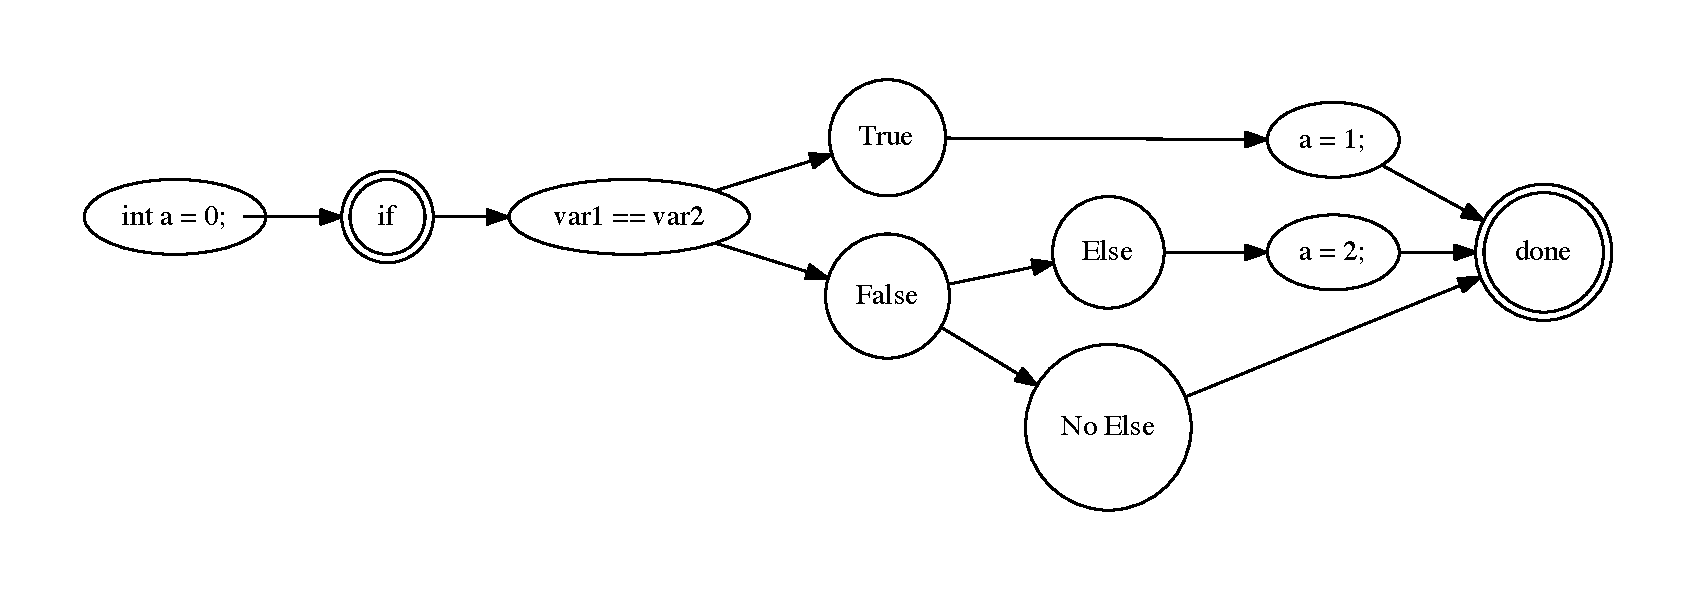
\includegraphics[width=\linewidth]{diagrams/if-flow.pdf}\\
\caption{General if and else statement flow of execution}
\end{figure}


An \Code{else} statement may be placed after an if statement, and any time the expression inside the parentheses following the \Code{if} is not true, the code inside the \Code{else} block is executed. 
For example:

\noindent\begin{minipage}{\linewidth}\begin{lstlisting}
if(variable == variable2)
{
  // Code here executes only when
  // the value of variable is the same as variable2
}
else
{
  // Code here executes if they are not the same
}
\end{lstlisting}\end{minipage}

An \Code{else} statement is used when you want some code to execute in any other case where the \Code{if} statement is not true. 
An example of how this works is also shown in Figure \ref{fig-if-flowchart}.

% \label{fig-else-flowchart}

An \Code{else if} could also be placed after the \Code{if} statement. 
An \Code{else if} is an additional \Code{if} statement checked only when the previous \Code{if} statement is false. 
While \Code{else} is a catch-all, \Code{else if} chains an \Code{if} to test for other conditions. 
Multiple \Code{else if} statements can be used, and they are all checked sequentially, and if necessary, an \Code{else} statement can be included at the end as a final catch-all. 
Take a look at Figure \ref{fig-else-if-flowchart} for a flowchart example.

% ^ I (Levi) personally think this is being taught wrong.


% \label{fig-else-if-flowchart}
\begin{figure}[h]
\label{fig-else-if-flowchart}
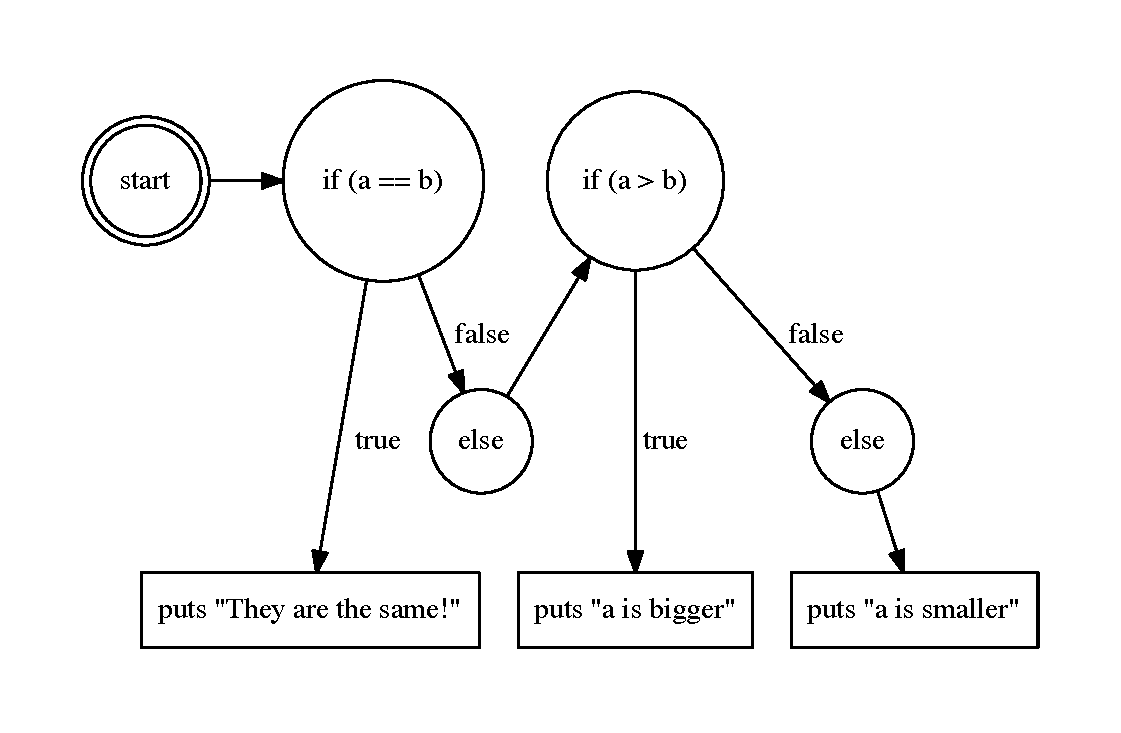
\includegraphics[width=\linewidth]{diagrams/if-else.pdf}\\
\caption{How if-else chaining works}
%TODO: Get this figure to be consistent with the style.
\end{figure}

Here's what the three statements would look like all together:

\noindent\begin{minipage}{\linewidth}\begin{lstlisting}
if(a == b)
{
  cout << "They are the same!" << endl;
}
else if(a > b)
{
  cout << "a is bigger!" << endl;
}
else
{
  cout << "a is smaller!" << endl;
}
\end{lstlisting}\end{minipage}

Note that every conditional expression is in parentheses. 
Conditional expressions also appear in loops (discussed in Chapter \ref{chap_loops}) and \Code{switch} statements.

\LevelD{\Code{switch} statements}

\Code{switch} statements (also sometimes called switch-case statements) make a menu-like set of blocks. 
It does the same job as many \Code{if} statements, but can simplify the job when used correctly. 
Here is an example:

\noindent\begin{minipage}{\linewidth}\begin{lstlisting}
switch(variable):
{
  case 1:
    //code to execute when variable is equal to 1
    break;
  case 2:
    //code to execute when variable is equal to 2
    break;
  default:
    //code to execute when variable is neither 1 nor 2
    break;
}
// Resume here after a break
\end{lstlisting}\end{minipage}

If \Code{variable} is equal to 1 then the code following \Code{case 1:} will be executed, if it is equal to 2, then the code following \Code{case 2:} will be executed, and if it is equal to neither, then the code following \Code{default:} will be executed. 
The cases are separated by \Code{break;}, which forces the code to leave the \Code{switch} statement's block of code.

This code:

\noindent\begin{minipage}{\linewidth}\begin{lstlisting}
switch(variable)
{
  case 1:
    cout << "You picked case 1. Lame.";
    break;

  case 2:
    cout << "Case two is way better.";
    break;

  default:
    cout << "WRONG!";
    break;
}
\end{lstlisting}\end{minipage}

\noindent is equivalent to this code:

\noindent\begin{minipage}{\linewidth}\begin{lstlisting}
if (variable == 1)
{
  cout <<  "You picked  case 1. Lame.";
}
else if (variable == 2)
{
  cout << "Case two is way better.";
}
else
{
  cout << "WRONG!";
}
\end{lstlisting}\end{minipage}

When there are only a few cases, \Code{if}, \Code{else if}, and \Code{else} statements are often easier. 
However, when you get to a greater number of cases, \Code{switch} statements become easier.

In \Code{switch} statements, only one \Code{case}'s code executes, provided that each \Code{case} is followed by \Code{break}. 
Otherwise, the program continues execution until it reaches a \Code{break} statement or the end of the \Code{switch} block. 
With an \Code{if} and \Code{else if}, only one branch may be executed, but the conditions in each \Code{if} are evaluated.

\begin{table}[bh]
		\begin{tabular}{| p{1.5in} | p{2.5in} |}
		\hline
			\textbf{User enters} & \textbf{Output} \\ \hline
			\Code{//Program start} &	<1> Addition \newline				<2> Subtraction\newline				             <3> Compare\newline							Type the number of your desired option: \\ \hline
			\Code{1} & The result of this addition is 9.3 \\ \hline
			\Code{2} & The result of this subtraction is 0.9 \\ \hline
			\Code{3} & A is greater than B \\ \hline
			\Code{//anything other than 1, 2, or 3} &	Not an option \\ \hline
		\end{tabular}
  \caption{The sample program's output}
  \label{table-conditional-program}
\end{table}


Here is some code that uses both \Code{switch} and \Code{if} statements.
Compiling and running the following code results in the output in Table \ref{table-conditional-program}.

\noindent\begin{minipage}{\linewidth}\begin{lstlisting}
#include <iostream>
using namespace std;

int main()
{
  int choice;
  double a = 5.1, b = 4.2;

  cout << "<1> Addition\n";
  cout << "<2> Subtraction\n";
  cout << "<3> Compare\n";

  cout << "Type the number of your desired option:\t";
  cin >> choice;

  switch(choice)
  {
    case 1:
	    cout << "The result of this addition is " << a + b << endl << endl;
	    break;

    case 2:
	    cout << "The result of this subtraction is " << a - b << endl << endl;
	    break;

    case 3:
      if (a > b)
		    cout << "A is greater than B";
      else if (a < b)
		    cout << "A is less than B";
	    else //a == b
		    cout << "A equals B";
	    break;

    default:
      cout << "Not an option";
      break;
  }

  return 0;
}
\end{lstlisting}\end{minipage}








\LevelD{Review Questions}
\begin{enumerate}
\item What is the output of the following code?

\noindent\begin{minipage}{\linewidth}\begin{lstlisting}
int a = 5;
int b = 10;

if(a > b)
  cout << "a is greater than b.";
else
  cout << "b is greater than a.";
\end{lstlisting}\end{minipage}

\item Why are \Code{switch} statements useful?

\item When are braces (\Code{\{\}}) needed in an \Code{if} statement?

\item Write a program that checks which number is higher than another and prints out an appropriate message. This program should use 2 variables, an \Code{if} statement and an \Code{else} statement. Bonus: Rewrite it to also check if the numbers are equal.

\end{enumerate}

\LevelD{Review Answers}

\begin{enumerate}
\item \Code{b is greater than a.}
\item \Code{switch} statements are useful for making menus for the user. (Other answers are also possible)
\item Braces are needed for any code longer than 2 lines following an \Code{if}.
\item \noindent\begin{minipage}{\linewidth}\begin{lstlisting}
#include <iostream>
using namespace std;

int main()
{
  int input1, input2;
  cout << "enter a number: ";
  cin >> input1;
  cout << "enter a number to compare to the first: ";
  cin >> input2;
  if(input1 > input2)
    cout << input1 << " is greater than " << input2;
  else
    cout << input2 << " is greater than " << input1;
}
\end{lstlisting}\end{minipage}

\end{enumerate}

\LevelD{Further Reading}

\begin{itemize}
\item ~
\item ~
\item ~
\end{itemize}	


     \LevelC{Strings}
			\label{chap_strings}
      % Strings

Let's discuss strings.
Strings are a data type typically used to hold a collection of printable characters such as words, sentences, or longer sequences.
In order to use strings in your program you must first include the string library:
\begin{lstlisting}
#include <string>
using namespace std;
\end{lstlisting}

\noindent Also note that a string, for convenience, can be treated like an array of individual characters.

When we declare variables of type \Code{string}, we declare them just like we would an \Code{int}, \Code{float}, or \Code{double}.
We can create a variable named \Code{myString} of type string by doing this:

\begin{lstlisting}
#include <string>
using namespace std;

string myString;
\end{lstlisting}

\noindent If you choose not to have \Code{using namespace std;} in your code, the variable \Code{myString} must be declared as follows:

\noindent\begin{minipage}{\textwidth}\begin{lstlisting}
#include <string>

std::string myString;
\end{lstlisting}\end{minipage}

\noindent We can then store anything we want in that string as long as it is made up of characters.
When a literal value is assigned to a string, it should be surrounded by double quotes such as in the case of \Code{"Hello"}:

\noindent\begin{minipage}{\textwidth}\begin{lstlisting}
#include <string>

string myString = "Hello";
\end{lstlisting}\end{minipage}

If we are storing the value of a string entered by a user, the user does not have to use quotes.
We can store \Code{"Hello"} in the string by doing the following:

\noindent\begin{minipage}{\textwidth}\begin{lstlisting}
string myString;
cin >> myString; // User types: Hello
                 // myString is now "Hello"
\end{lstlisting}\end{minipage}

\noindent It is also possible to use the arithmetic operator \Code{+} with strings to concatenate (combine) the two strings.
If we combined one string that contained \Code{"Hello"} and another string that contained \Code{"World"} the connected string would then read \Code{"HelloWorld"}.

\noindent\begin{minipage}{\textwidth}\begin{lstlisting}
string v1 = "Hello",
       v2 = "World";
cout << v1 + v2 << endl;
// Outputs:
// HelloWorld
\end{lstlisting}\end{minipage}



In order to have a space between the two words, one of the strings would need to contain a space such as this:

\noindent\begin{minipage}{\textwidth}\begin{lstlisting}
string v1 = "Hello", v2 = " World";
//-------------------------^-------
cout << v1 + v2 << endl;
// Outputs:
// Hello World
\end{lstlisting}\end{minipage}

\noindent Or it can be represented as: 

\noindent\begin{minipage}{\textwidth}\begin{lstlisting}
string v1 = "Hello ", v2 = "World";
//----------------^----------------
cout << v1 + v2 << endl;
// Outputs:
// Hello World
\end{lstlisting}\end{minipage}

\noindent Alternatively, a space can be added like so:

\noindent\begin{minipage}{\textwidth}\begin{lstlisting}
string v1 = "Hello", v2 = "World";
cout << v1 + " " + v2 << endl;
//------------^-------------------
// Outputs:
// Hello World
\end{lstlisting}\end{minipage}

\noindent The first two concatenates the two strings to create one string that contains ``Hello World'', and the third concatenates three strings to produce the same result.

When reading strings from \Code{std::cin}, the default behavior is to collect all characters until the first whitespace (a tab, space, or newline) character that it finds in the input.
For example, if the user inputs ``Hello World'' in the following code, \Code{std::cin} stops reading at the first whitespace, and thus the string would contain only ``Hello''.
If we want to read the entire line of text, we need to use the \Code{getline()} function, which reads until the first newline character.
This is how you use the \Code{getline()} function:

\noindent\begin{minipage}{\textwidth}\begin{lstlisting}
string myString;
getline(cin, myString);
\end{lstlisting}\end{minipage}

\noindent This function call will take the entire line of input, including all whitespace characters, and store it in the variable \Code{myString}. 
		
We can also find out the length of the string by using the member function \Code{length()} with any \Code{string} object.
For example, if we wanted to find the length of a string entered by a user and store it in a variable named \Code{stringLength}, we might do this:

\noindent\begin{minipage}{\textwidth}\begin{lstlisting}
string myString;
int stringLength;
getline(cin, myString);
stringLength = myString.length();
cout << "The string you entered was "
     << stringLength
     << " characters long."
     << endl;
\end{lstlisting}\end{minipage}

\noindent Aside from finding the length of a string, we can search for certain characters in the string by using the \Code{find()} and \Code{rfind()} member functions.
For example, if we wanted to find a single space in a string variable named \Code{myString} that contains ``Hello World'', we would do this:

\noindent\begin{minipage}{\textwidth}\begin{lstlisting}
string myString = "Hello World";
int spot = myString.find(" ");
\end{lstlisting}\end{minipage}

This code results in the value 5 being stored in the variable named \Code{spot} because the space character at index 5 if you treat the string as an array, as shown in Figure \ref{fig-stringfind}.
% TODO: Where did this figure come from? It was referenced in the text, but no such graphics or figures were presented.
Remember that we start at index 0, so even though the space is in the sixth position, it is at index 5 in the string.
When a line of text is stored in a string, think of it as being stored in memory in an array of the same length as there are characters in the string.
For example, the string ``Hello World'' can be contained in an array with 11 slots, therefore the space character would be found in \Code{myString[5]}.
The \Code{find()} function can also search within a string from some arbitrary starting point, instead of from the beginning:

\noindent\begin{minipage}{\textwidth}\begin{lstlisting}
string myString = "Hello World";
int spot, spot2;
spot = myString.find(" "); // found at index 5
spot2 = myString.find("o", spot); // starting from index 5, found at index 7
\end{lstlisting}\end{minipage}

\noindent The second argument that is passed to the function (in this case, \Code{spot}) is the index at which you want to start your search.

We can also use the \Code{rfind()} function to find a character in reverse direction from the end of the string, or from some starting point, as above.
If we wanted to find the single character string \Code{"o"} before the space we might do something like this:

\noindent\begin{minipage}{\textwidth}\begin{lstlisting}
string myString = "Hello World";
int spot, spot2;
spot = myString.rfind(" "); // found at index 5
spot2 = myString.rfind("o", spot); // starting from index 5, found at index 4
\end{lstlisting}\end{minipage}

\noindent This function call to \Code{rfind()} uses the arguments \Code{"o"} and \Code{spot}.
This stores the position of the first \Code{"o"} it comes across after going in reverse from the index stored in \Code{spot} (which contains 5).
This would be equivalent to the last line:

\noindent\begin{minipage}{\textwidth}\begin{lstlisting}
spot2 = myString.rfind("o", 5); // starting from index 5, found at index 4
\end{lstlisting}\end{minipage}

\noindent Both of these function calls will start searching for the string \Code{"o"} backwards from the same spot in the string, at index 5. 

Sometimes the string you search for cannot be found, as in this example:

\noindent\begin{minipage}{\textwidth}\begin{lstlisting}
	string myString = "Hello World";
	int spot = myString.find("Q"); // No Q in this string!
\end{lstlisting}\end{minipage}

\noindent In this case, the \Code{find()} (or \Code{rfind()}, for that matter) returns a special value named \Code{string::npos}.
When we use \Code{find()} or \Code{rfind()} and believe that they could fail, we should verify that the string was found, as below:

\noindent\begin{minipage}{\textwidth}\begin{lstlisting}
string userInput;
int spot;
cin >> userInput;
spot = userInput.find("Z");

if (spot == string::npos)
	cout << "There was no Z in what you typed!" << endl;
else
	cout << "The first Z was in position " << spot << endl;
\end{lstlisting}\end{minipage}
\LevelD{Review Questions}
\begin{enumerate}
\item Write code to declare a string and take input from a user.
\item Can a string be treated as a character array?
\item When do you use a string?
\item What is the \Code{\#include} needed to use strings?
\item What function do you have to use to take an input with a space?
\end{enumerate}

\LevelD{Homework Questions}
\begin{enumerate}
\item Write a code that takes in 5 words and outputs them 4 times.

\item Write a program that takes in the following words: King, Queen, Knight, Bishop, Rook, Pawn. 
Then it has to switch the King with the Pawn, the Rook with the Queen, and the Bishop with the Knight.
It must output the original data in the original order, and output the data once it is all finished.

\item Write a game program where the user inputs 4 different words, then the user gets 4 guesses to guess all of the words they originally inputted.
This program should run as many times as the user wants.
\end{enumerate}

\LevelD{Review Answers}

\LevelD{Homework Answers}

\LevelD{Further Reading}
\begin{itemize}
\item \url{http://www.harding.edu/fmccown/cpp_strings.pdf}
\item \url{http://www.stanford.edu/class/cs106x/handouts/08-C++-Strings.pdf}
\end{itemize}

     \LevelC{Loops}
      \label{chap_loops}
      \LevelD{Introduction}

Okay, so you know how to do some programming, but now you need to be able to handle a dozen or more operations that are obnoxiously repetitive.
Imagine that you have a program that needs to allow data to be entered about your employees.
Do you really want to have to write out the code to do that for every single individual?
No---you want to set it up so you write it out as concisely as possible, and copy and paste just won't work.
What we need to do is write the relevant code once and have it repeated for us as many times as necessary.

For this, we'll use a structure known as a \Keyword{loop}, which does exactly what you expect it would.
A loop allows you to repeat a section of code as many times as you need.
When the code reaches the end of the section, it goes back to the top of the section and the loop starts again.
After each repetition of the loop (which we call an \Keyword{iteration}), it will check for an \Keyword{end condition} that is specified by the programmer. 

\LevelD{Having Fun \Code{while} Programming}

The first loop we'll cover is the \Code{while} loop, probably the simplest and easiest-to-use loop.
It's referred to as a \Keyword{pretest loop} as it's designed to check the loop's end condition prior to a repetition of the loop.

Figure X-1: Logic of a while loop
% TODO: Logic for a while loop
\label{fig-while-logic}

In Figure \ref{fig-while-logic}, the basic model of a "pretest loop" is shown.
A diamond is used to represent where a decision must be made.
In this case, it's a Boolean expression.
If the expression is true, control passes to the rectangle, which represents an action (or actions) to be performed: the statements that represent the body of the loop.

As with everything else we've learned so far, syntax is important. The structure is simple enough, as the pseudocode below shows:

\begin{lstlisting}
while (BooleanExpression)
{
	statement;
	statement;
	// whatever else needs to be done
}
\end{lstlisting}

The important thing to remember here is to be sure you have some statement to eventually allow the loop to exit.
When the Boolean expression is false, remember, the loop is finished.

Also, note that, like an \Code{if} statement, the braces are not necessary if there is only one statement following the line with the \Code{while} keyword and Boolean expression.
Is it recommended to use the braces with only one statement?
For your own sanity, and that of others reading your code, yes.
Do you have to?
No, but some organization's coding standards might say otherwise, because it makes the code easier to read and edit.
So remember, it's best to start with good habits early.

Now, lets look at an actual example of a \Code{while} loop.

\begin{lstlisting}
int i = 10;	//initializes i at 10

cout << "T-minus ";
while(i>=0)	// while loop that is ended when i is less than 0
{
	cout << i << endl;	//outputs the value of i, then moves to a new line
	i--;	//decreases the value of i by 1
};

cout << "Lift Off!";
\end{lstlisting}

This code prints a countdown:

\begin{lstlisting}
10
9
8
7
6
5
4
3
2
1
Lift Off!
\end{lstlisting}


\LevelD{\Code{do}-\Code{while} Loops}

Remember how the \Code{while} loop is known as a pretest loop?
Well, a \Code{do}-\Code{while} loop is known as a \Keyword{post-test loop} for a similar reason.
Let's take a look at the flowchart in Figure \ref{fig-do-while-logic} and take a guess.

Figure X-2 Logic of the do-while Loop
% TODO: Figure for a do-while loop
\label{fig-do-while-logic}

Post-test loops perform the statements in the body of the loop \emph{before} it tests the end condition.
Let's look how this will affect the syntax you will use when implementing the loop.

\begin{lstlisting}
do
{
	something;
	something;
	// whatever else needs to be done
} while (BooleanExpression)
\end{lstlisting}

The difference between a \Code{while} and a \Code{do}-\Code{while} loop is where each checks its end condition.
In this case, the line with the \Code{while} and the end condition are after the main section of code.
In a normal \Code{while} loop, the program can potentially meet the end condition before even entering the loop body, and just pass over it.
In a \Code{do}-\Code{while} loop, the program checks the end condition after each iteration of the loop, so it will run at least once before the loop ends.

There's not a whole lot more to add then hasn't been stated in the while loop section, so lets take a look at an example.

\begin{lstlisting}
    char cont; //short for continue; continue is a key word and can't be used

    do {

    cout << "Go Cadets!\n";

    cout << "Do you want to continue? Type Y for yes: \t";
    cin >> cont;

    } while (cont == 'Y');
\end{lstlisting}

\LevelD{Event-Based Loops vs Count-Based Loops}

Loops can be organized into two categories based on how you use them.
These two categories are defined by if you want to do a certain number of iterations of the loop (a \Keyword{count-controlled} loop) or continue until some event occurs, such as a particular user input (an \Keyword{event-controlled} loop).
Let's look at code examples to differentiate the two. The first example shows an event-controlled \Code{while} loop.

\noindent\begin{minipage}{\linewidth}\begin{lstlisting}
int sum=0, temp; //declares sum and temp. Initializes sum to 0.

cout << "Please give a number to add: ";
cin >> temp;	//has user input the temporary variable to add to sum

while (temp != 0) 
{
	sum += temp;	//sets sum equal to sum+temp at start of loop
	cout << endl << "total: " << sum << endl;	//outputs sum total
	cout << "Add another number? If yes, input an integer greater than or less than 0. "
<< "If no, input 0." << endl;	//asks user to input temp variable again
cin >> temp;
}
\end{lstlisting}\end{minipage}

\noindent This example shows a count-controlled \Code{while} loop:

\begin{lstlisting}
    int counter = 1;

    while(counter != 12)
    {
        cout << counter << endl;
        counter++;
    }
\end{lstlisting}

\LevelD{\Code{for} work or \Code{for} play}

Consider what we have needed for each loop we've covered.
We've needed to initialize a variable that we want to check.
We've also needed an end condition to test that variable against.
Finally, we needed a way of modifying that variable to meet that end condition.
After that, it's whatever we've felt like putting in. With the \Code{for} loop, we put those three elements into the loop header, separated by semicolons (\Code{;}).
A \Code{for} loop would would look something like this:

\noindent\begin{minipage}{\linewidth}\begin{lstlisting}
for(IntializationExpression; TestExpression; UpdateExpression)
{
	something;
	something;
	// whatever else you need
}
\end{lstlisting}\end{minipage}

The \Code{for} loop by its nature lends itself to being a count-controlled loop.
You use this kind of loop to count up (or down) each iteration until you get to the specified value. 

Let's run through how a \Code{for} loop should run, following Figure \ref{fig-for-logic}.
Assuming everything is correct, you would initialize the first value to something such as an \Code{int counter} that is set to 1.
The \Code{TestExpression} will include the same Boolean logic you would use in \Code{while} and \Code{do}-\Code{while} loops, so let's just say when \Code{counter} is less than or equal to 5, the loop will terminate.
Finally, let's say  \Code{counter++} is the update expression.
In each iteration (unless you also decide to change \Code{counter} from the body of the loop) you will move through this pretest loop four times.

Figure X-3 Logic of a for loop


\label{fig-for-logic}
% TODO: Figure for the for loop needs to be done.

\noindent This code corresponds to the logic in Figure \ref{fig-for-logic}:

\begin{lstlisting}
    for(int counter = 1; i <= 5; i++)
    {
        cout << i << endl;
    }
\end{lstlisting}

\noindent ...which produces the following output:

\begin{lstlisting}
1
2
3
4
5
\end{lstlisting}

\LevelD{Picking a Loop}

Which loop you use is dependent on your preferences and needs.
A \Code{for} loop is nice, but it's more convenient as a count-controlled loop.
If you needed to use an event-controlled loop, you may prefer to use a \Code{while} or \Code{do}-\Code{while} loop.
A \Code{for} loop is a nice way to condense the initialization, end conditions and update statement of the loop into one short line.
When choosing between a \Code{do}-\Code{while} and a \Code{while} loop, you should remember that with a \Code{do}-\Code{while}, it will always run at least once, while a \Code{while} loop may run zero or more times.

\LevelD{Nested Loops}

Much like \Code{if} statements, loops can be nested within each other.
Just remember to practice good formatting habits to keep the code from being too confusing.
Take a look at the example below, then let's talk our way through it.


\begin{lstlisting}
for(int hours=0; hours<24; hours++)	//a single day
{
	for(int minutes=0; i<60; minutes++)	// a single hour
	{
		for(int seconds=0; seconds<60; seconds++)
			//a single minute
		{
			cout << hours << ":" << minutes
 << ":" << seconds << endl;
//outputs the current time
		}
	}
}
\end{lstlisting}

For those readers who concluded that this is a clock simulation, you are correct!
Our system of time is set up that we have 24 hours in a day, and each hour needs to go through a 60 minute cycle, and each minute has a 60 second cycle.
The code mimics this by advancing the seconds 60 times before advancing each minute.
After 60 minutes, the hour counter loop is incremented. Each time an outer loop starts another iteration, variables inside the inner loops are reset.

Infinite Loops

Remember to have some way of advancing towards the end condition.
What will happen if you can't reach that end condition from within the loop?
Most likely an infinite loop will occur. And what exactly is an infinite loop?
If you said it's a loop that can't stop itself, then you would be right.
Depending on the operation of the loop, you may not know what is happening, and this could potentially cause disastrous results.
Let's look at an example of a \Code{while} loop that suffers from an infinite loop.

\begin{lstlisting}
    int counter = 1;

    while(counter != 12)
    {
        cout << counter << endl;
        counter += 2;
    }
\end{lstlisting}

Because \Code{counter} starts with a value of 1, and adds 2 each time the loop executes, \Code{counter} will always be odd, and never equal twelve.
Therefore, the loop will never end.

\LevelD{Review Questions}
\begin{enumerate}
\item Create a while loop that increments some integer variable \Code{x} initialized with a value of 0 by 3 until the value of \Code{x} reaches a value of 30.
Make sure you declare the variable and initialize it first! 

\item  Create a do-while loop that reads integer values given by the user into an integer variable \Code{x}, initialized to 0, then adds those values onto some variable named \Code{totalVal} until \Code{totalVal} reaches at least 20.

\item Create a for loop that outputs your name to the screen 10 times before exiting the loop.

\item What is wrong with the following code?
\begin{lstlisting}
for (int j = 10, j > 0, j--)
	{
		cout << j << endl;
		if (j = 1)
		{
			cout << "BOOM!\n";
		}
	}
\end{lstlisting}

\item In the last question, was the loop an event-controlled loop or count-controlled loop?
\end{enumerate}


\LevelD{Homework Questions}
% TODO: Homework Questions
\LevelD{Review Answers}
\begin{enumerate}

\item
\noindent\begin{minipage}{\linewidth}\begin{lstlisting}
int x = 0;
while (x < 10)
{
	x++;
} 
\end{lstlisting}\end{minipage}

\item
\noindent\begin{minipage}{\linewidth}\begin{lstlisting}
int x = 0;
int totalVal = 0;
do
{
	cout << "Type in a number: "; 
	cin >> x;
	totalVal += x;
}
while (totalVal < 20); 
\end{lstlisting}\end{minipage}

\item 
\noindent\begin{minipage}{\linewidth}\begin{lstlisting}
for(int i = 0; i < 10; i++)
{
	cout << "Your name here\n";
}
\end{lstlisting}\end{minipage}

\item
\noindent\begin{minipage}{\linewidth}\begin{lstlisting}
for (int j = 10; j > 0; j--)
{
	cout << j << endl;
	if (j == 1)
	{
		cout << "BOOM!\n";
	}
}
\end{lstlisting}\end{minipage}

\item Count-Controlled

\end{enumerate}


\LevelD{Homework Answers}
% TODO: Homework answers
\LevelD{Further Reading}
Basic Loops:
\begin{itemize}
\item \url{http://www.cplusplus.com/doc/tutorial/control/}
\item \url{http://www.cprogramming.com/tutorial/lesson3.html}
\end{itemize}

\noindent Ranged-Based Loops
\begin{itemize}
\item \url{http://www.cprogramming.com/c++11/c++11-ranged-for-loop.html}
\end{itemize}



     \LevelC{Arrays}
			\label{chap_arrays}
      Array 

% Add std::array in a future version

\Comment {

What is it, how they work?
	An array is a series of variables that are the same of the same type (int, float, double, char etc�). Arrays are held in a computer's memory in a strict linear sequence. An array does not hold anything other than the elements of the specified type. So there is no assigning an array of type float and hoping to store a string there. Doing so would cause a "type mismatch error" and the program wouldn't compile. To create an array, the user types into their compiler 
(data type) (array name)[(length of array)];
A concrete example looks like: 
	char Scott [5];
The char is the data type for all elements in the array, Scott is the name of the array (you can be as creative as you want with the name) and the 5 inside the square brackets represents the size of the array. So char Scott [5] can hold 5 pieces of data that are of type char. Look at the diagram below for assistance.
When trying to visualize an array, think of a rectangle split up into as many open slots as the user defines. In the case of the above example, think of a rectangle with 5 open slots, each of type char that are waiting for some form of input. 



In order to refer to the individual elements in an array, we start with the number 0 and count upwards. We use [0] to access the first element in the array, [1] for the second, [2] for the third, and so on. In order to read or write certain locations of the array, we state the name of the array and the element we want to call. It should look like this (refer to the diagram to visualize how the computer interprets this).
Scott[3] = 'Q'; // editor's note - make this a single apostrophe
cout << Scott[3];









You can also store values inside the array ahead of time when you are declaring the array. To do so, you need to enclose the values of the appropriate type in brackets and separate the values with a comma. Below are two examples, one of type char and one of type int.

char Scott [5] = {' S', 'c', 'o', 't', 't'};	










int John [5] = {99, 5, 1, 22, 7};

	

	Note that, in the C and C++ language, arrays of characters intended to be printed must contain a special character called the null character or null terminator. In the language, this character is represented by '\0'. The null character marks the end of the array and may be put in the last slot in the array, after any printable characters. Because the null character takes up one slot on its own, any character array should be declared as at least one space larger than the longest string that you expect to store.

	char witch_doctor[10] = {'v', 'o', 'o', 'd', 'o', 'o', 'b', 'a', 'd'};
	cout << witch_doctor[7];














Multi-dimensional Arrays
A two dimensional array (some might call it a "matrix") is the same thing as an array, but is an "array of arrays." Here's a two-dimensional three-by-three array:
int Rich [3][3] // 2D
Declaring arrays with more dimensions are possible with similar syntax. Here's a three-dimensional 10x10x10 example:
int Sam [10] [10] [10] // 3D
And a four-dimensional 10x10x10x10 array. This is possible, even though it's hard to visualize.
int Rich [10] [10] [10] [10] // 4D�etc
A user can input values into a multi-dimensional array in a similar way as with a single-dimensional array. 
int main()
{
    int neo[3][3] = { {1,2,3}, {4,5,6}, {7,8,9} }; // filling matrix with set numbers
    cout << neo[0][0] << endl <<endl; // first number, 1
    cout << "  " << neo[2][2]; // last number, 9
    return 0;
}

















	The same logic is applied for 3 dimensional and 4 dimensional arrays, but when filling them, be mindful of the order of the input so that when you want to view certain elements in the array you are able to correctly access them.


References: 
Other examples on filling array/matrix
1) http://www.cplusplus.com/forum/beginner/43663/
2) VIDEO https://www.youtube.com/watch?v=SFGOAKYXfOo
3) http://visualcplus.blogspot.com/2006/03/lesson-15-matrixes-and-2d-arrays.html

Making a array/matrix inside a pointer
1) http://stackoverflow.com/questions/256297/best-way-to-represent-a-2-d-array-in-c-with-size-determined-at-run-time
2) http://forums.devarticles.com/c-c-help-52/c-pointer-to-multidimensional-array-11075.html

}
     \LevelC{Blocks, Functions, and Scope}
			\label{chap_functions}
      \LevelD{Blocks}

Since we've covered \Code{if} statements and loops, let's go into more detail about the code that's contained within them. 
When you need to contain multiple lines of code, we've shown how to use braces. 
These braces will create a new layer in the code, and the lines within would be grouped into what is known as a compound statement, sometimes called a block.

\begin{lstlisting}
  int x;
  cin << x;

  if(x < 5)
  {
    int y;
    cin << y;	
    x += y;	//Declares Y, asks user to define Y, then sets Y to X + Y
  }

  if(x > 5)
  {
    int z;
    cin << z;
    x -= z;	//Declares z, asks user to define z, then sets x to x - z
  }

  cout >> x;
  //outputs either x-z, x-y, or 5
\end{lstlisting}

Take a look at the example above. 
There are two blocks here: the one for if \Code{x} is less than 5, and the one for if \Code{x} is greater than 5. 
Notice the variables declared in each, \Code{y} and \Code{z}. 
When these are declared, they are only usable within the blocks that they were declared. 
When that block reaches its end, they are lost to the rest of the program. 
This is because the scope of the variables within the blocks is limited to those blocks.
We discuss scope further at the end of this chapter.

\LevelD{Basic Functions in C++ }
 
\LevelE{What are Functions and why do we use them?}
 
Functions are an important part of C++ programming. 
Without them, programs would be confusing and difficult to troubleshoot. 
When programs are written, they tend to be written in logical chunks which we call subprograms. 
These subprograms are known as functions in C++ which, when called in a program, may execute whatever the programmer wants. 
Simply put, functions are like miniature programs that when pieced together form the actual program that you are trying to write.
 
\LevelE{The parts of a basic function}
 
A \Keyword{function declaration} (sometimes known as the \Keyword{prototype}) is normally placed before the \Code{main()} function in your code. 
This lets the compiler know that there is a function that will be defined in more detail further on in your program. 
With basic functions, your declarations should start with a \Keyword{return type} such as \Code{double}, \Code{int}, and so on; this is the data type your function will return. 

After the return type, the next item that needs to be written is the function's name, which can be almost anything you want. 
Remember that you will be using it again later in your code, so it makes sense to make it something short and logical that you can remember! 
Now that you have your data type and your function name, it's time for zero or more function \Keyword{parameters}. 
These will be written inside parentheses immediately following your function's name. 
Each parameter is in turn made up of a data type and a name like a variable declaration. 
A comma separates function parameters and your declaration must end with a semicolon after the closing right parenthesis.

Here is an example of a function declaration:

\begin{lstlisting}
double profit (int cost, double price); //cost and price are parameters.
\end{lstlisting}
        	
Using function looks much like an abbreviated version of the function declaration. 
A \Keyword{function call} is responsible for telling the compiler when and how to execute a function.
Function calls are found in another function like \Code{main()}. 
Often the user is prompted to enter necessary data with \Code{cout} statements and his or her response is collected with \Code{cin}. 
Once this data is collected, the program holds it until a function call is made somewhere in the code.
Once the function call is made, the compiler takes the entered data and then uses the code in the \Keyword{function definition} (which we will go over shortly) to operate on the parameters and return a value. 
For your function call, write your function name followed by the variables or values you want to pass in.
In a functiton call, it is not necessary to specifty the data types, as they are already understood.
 
Here is an example of a function call:

\begin{lstlisting}
#include <iostream>
 
using namespace std;
 
double profit (int cost, double price); // function declaration (prototype)
int main ()
{
 
  double a, b;
  int c;
  cout << "Enter the manufacturing cost of the item: ";
  cin >> c;
  cout << "Enter the retail price of the item: ";
  cin >> b;
 
  a = profit (c, b); // function call profit with cost = c and price = b
  cout << a << endl;
  return 0;
}
\end{lstlisting}
  
You have a declaration and a function call now. 
The only thing left is the code inside the function definition---the \Keyword{function body} is the most important part because it contains the code needed by the compiler to execute the function.

The function definition will usually have a lot more code than both the declaration and the function call.
As a result, the definition and body are also more difficult to write than the declaration or call. 
The function definition and body is often placed after your \Code{main()} function. 
Multiple function definitions and bodies can be placed after your \Code{main()} in no particular order, though it makes it less confusing if you use the same order as when they were declared.  
Start your function definition with your \emph{function heading}, which looks exactly like your function declaration but without a semicolon. 
Following your heading, you need your function body. 
Start your function body by placing an opening left brace (\\Code{\}}) on the line following your heading. 
The code that makes up the function body follows the brace.
After the code in the body is finished, you end the body with a closing right brace (\\Code{\{}). 
Notice that the semicolon is not necessary either after your heading or after your closing brace. 
The standard rules for semicolons apply within the body of the function, though.  
What goes inside the function body depends completely on what you want the function to do. 
You may declare variables to be used just in your function and can leave the function using \Code{return} statements at any time. 
Below is an example of a function definition:

\begin{lstlisting} 
double profit (int cost, double price) // function definition
{
  double p; // temporary variable
  p = price � cost; // calculate the profit
  return p; // return the result to the calling function
}
\end{lstlisting}
 
Great, now that you have a grasp of the three major parts of basic functions we can move on to other related material!
 
The functions we just described are known as \Keyword{programmer defined functions} since the programmer defines these functions. 
There are also \Keyword{predefined functions} which are available for your convenience. 
Predefined functions are functions that are already written and defined. 
In order to use predefined functions, the programmer needs to include the necessary library and then call the function wherever they need it.

In the following example we will use the \teCodexttt{sqrt()} function to calculate the square root of the user's input. The \Code{sqrt()} function is described in more detail in Chapter \ref{chap_advancedarith}.
 
\begin{lstlisting}
#include <iostream>
#include <cmath>
 
using namespace std;
 
int main()
{
  double num;
  cout  << "Please enter a number: ";
  cin >> num;
  cout << sqrt(num) << endl;
  return 0;
}
\end{lstlisting}
 
\LevelD{\Code{void} Functions}
 
\Keword{\Code{void} functions} are functions that do not return a value. 
Notice that other function declarations that do return a value start with their return type such as: \texttt{double}, \texttt{int}, or the like. \texttt{void} functions behave the same except no value is returned. A common application where a \texttt{void} function is used is printing the result of calculations to the screen. The calculations might be performed elsewhere, but the results would be printed using the \texttt{void} function. Syntax for \texttt{void} functions works in the same way as normal functions, but \texttt{void} is written where the return data type would normally go. The declaration, function call and definition for \texttt{void} functions will follow the same format as other functions. Note that, like other functions, there does not necessarily need to be parameters in a \texttt{void} function.

Here is an example of a simple void function declaration:

\begin{lstlisting}
void displayMessage();
\end{lstlisting}

Remember the definition and calling of void displayMessage() would be the same as any other function with the exception of the \texttt{void} return type and that no value is returned!

\LevelD{Overloading Function Names}

Overloading function names allows the same name to be used in multiple function definitions but with different parameter listings. Function names can be reused using this feature. Function name overloading eliminates problems associated with having multiple names for multiple functions with similar purposes and can make the code both more understandable and more convenient for the programmer to write.

Below is an example of an overloaded function name. Notice that both functions have the same name, but different parameter types.
\begin{lstlisting}
int plus( int num, int numr);
float plus(float num, float numr);
\end{lstlisting}

Here is an example of improper function overloading. Simply changing the return type does not work, the parameters must be different!

int plus(int num, int numr);
float plus(int num, int numr);  



\Comment {

\LevelD{Scope}

As we dive into more complex programs there is a need for a wide variety of variables in different locations in the code. 
Some of these variables are declared within individual blocks of code, such as within loops or conditionals. 
Others are declared completely outside functions. 
The two primary types of variables we are going to look at here are local and global. 
The location of the declaration of a variable within the code changes how that variable may be used.
	
Local variables are declared within a block of code. 
A local variable is available to code from the point of its declaration through the end of that block of code. 
A simple example is a variable declared in \Code{main()}:

\begin{lstlisting}
int main()
{
  int games;
  // Other code here
  return 0;
}
\end{lstlisting}

The variable \Code{games} is a \Keyword{local variable} because it exists only within the local function, \Code{main()}. It cannot be used anywhere outside \Code{main()} without some additional work (such as passing it by reference to another function). Similarly, variables declared in other functions are not available to code in \Code{main()}. Here is an example:

\begin{lstlisting}
#include <cstdlib>
#include <iostream>

using namespace std;
	
void my_games();

int main()
{
		my_games();
		// More code here
		cout << games; // ERROR! No such variable here!
		return 0;
}

void my_games()
{
	int games = 10;
		cout << games;
}

	In the previous example function, \Code{my_games()} is called by \Code{main()} and outputs \Code{10}. The variable \Code{games} is local to that function. If \Code{games} is referenced anywhere else outside that function, the program will not compile.

An easy way to understand local variables is to compare them to your neighbors. Everyone that lives on your street and around you are variables, and since you all share the same street, they are local. The neighbors on an adjacent street might be close to where you live, but since they do not share the same street, they might not be considered neighbors. You can think of these neighbors on the adjacent street as other functions. While they might be close by, they do not share the same street.

	Global variables are quite different from local variables. Global variables can be used by code anywhere within the program. A global variable is declared outside of any function. Using similar code as in the example above, we make the \Code{games} variable global:

#include <iostream>
#include <cstdlib>

using namespace std;

void my_games();
void their_games();

int main()

{
	games = 5;
		my_games();
		their_games();

		return 0;
}

void my_games()
{

		cout << games << endl;
}


void their_games()
{
	cout << games << endl;
}


Both functions print the same variable, causing the program to produce the following output: 


5
5


To sum it up, local variables work only within the block of code that it is declared. Global variables are declared outside functions, and can be used at any point in the program.



}




     \LevelC{Problem Solving \& Troubleshooting}
			\label{chap_problems}
      % This work by Jeremy A. Hansen is licensed under a Creative Commons 
% Attribution-NonCommercial-ShareAlike 3.0 Unported License, 
% as described at http://creativecommons.org/licenses/by-nc-sa/3.0/legalcode

Problem solving and troubleshooting in programming is often referred to as debugging. 
Does your program not compile? 
Does it not achieve the desired effect? 
Debugging is your answer. 
And, unless you are a perfect programmer, you are likely to do quite a bit of debugging.

The first step to debugging is looking for common errors.

\LevelD{The Compilation Error}

These errors happen when your compiler returns an error message after you hit compile. 
The messages usually tell you what is wrong, and what line the error is on, but be sure to double-check the lines immediately before and after the reported error. 
Because the code is incorrect, the compiler can only guess at what you meant and give you a hint.

\begin{figure}[tbh]
  \centering
  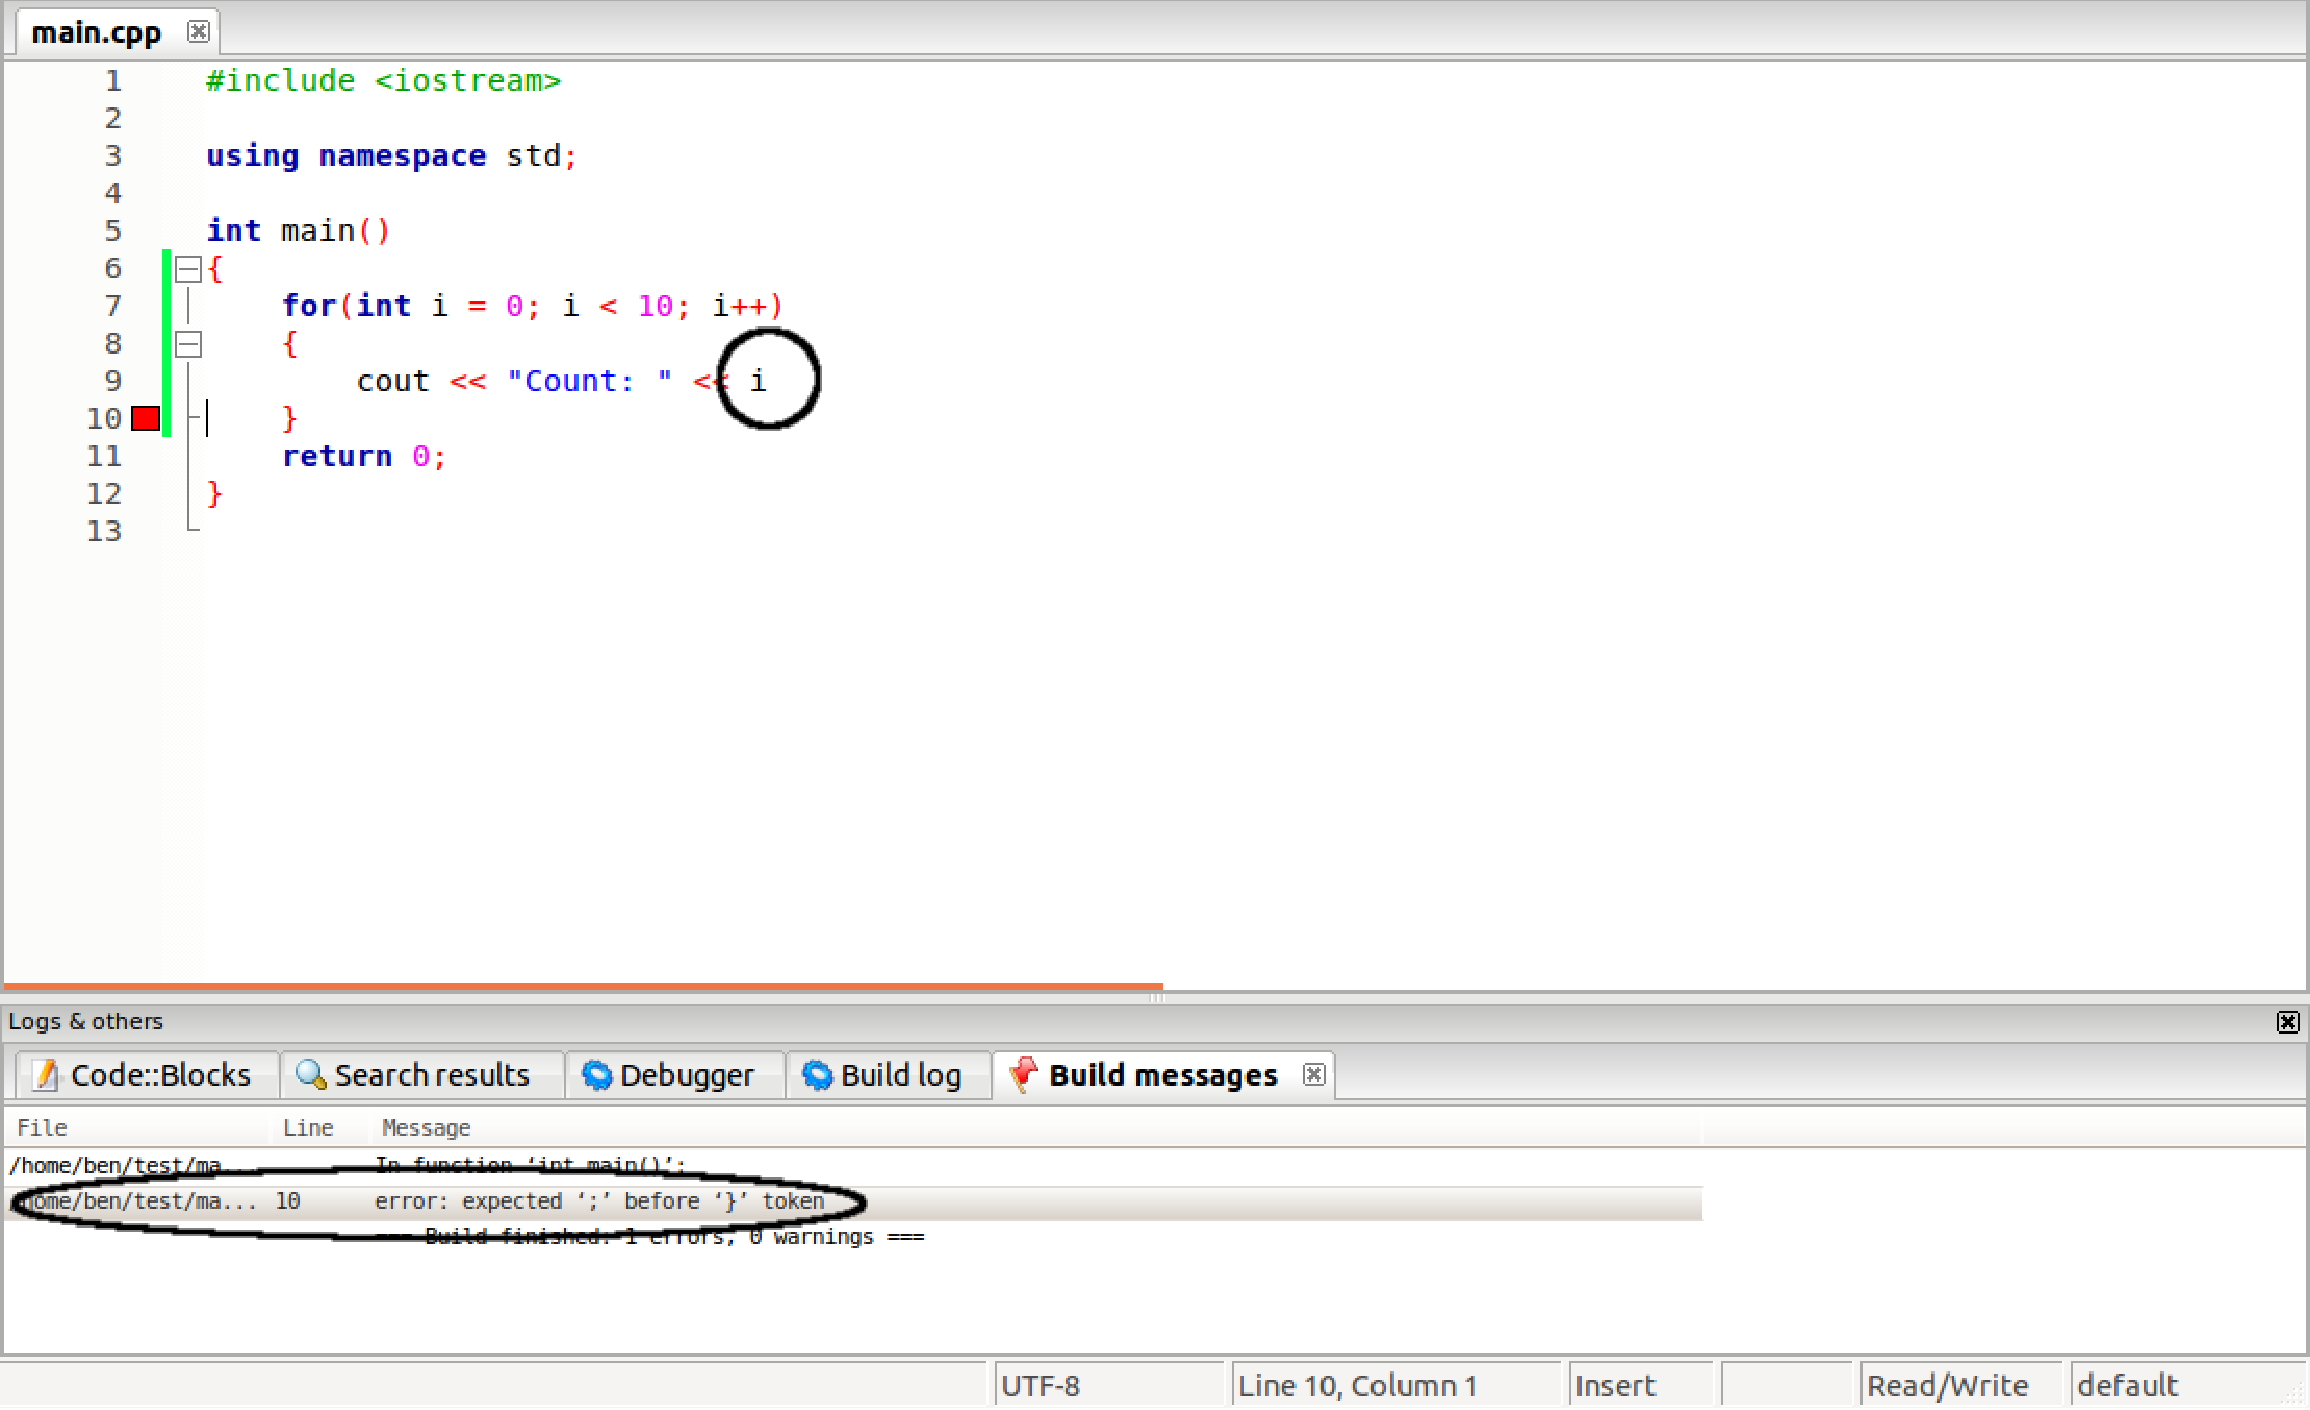
\includegraphics[width=\textwidth]{diagrams/fig-netbeans-syntax-error.pdf}
  \caption{A syntax error in the NetBeans development environment} \label{fig-netbeans-syntax-error} 
\end{figure}

For example, one of the most common errors a beginning programmer will encounter is forgetting a semicolon. 
In some development environments (like NetBeans in Figure \ref{fig-netbeans-syntax-error}), this will cause the error to be reported not on the line with the missing semicolon, but on the following line. 

\LevelD{The Logic Error}

Logic errors are often subtle, and occur after the code compiles. 
When the code is executed, however, the result is wrong. 
This may happen when arithmetic operators like \Code{+}, \Code{-}, \Code{*}, and \Code{/} get mixed up. 
Another common issue is misplacement of parentheses, as a misplaced parenthesis can cause problems in complex expressions. 

\LevelD{The Infinite Loop}

Another specific logic error is the infinite loop. 
The infinite loop is a common error that can result in your program repeating the same block of code over and over. 

For an infinite loop to occur, the conditional expression of a \Code{while}, \Code{for}, or \Code{do-while} loop remains true. 
There are many ways for this to happen, such as accidentally using \Code{=} instead of \Code{==} to compare two numbers, or using the wrong operators, like a \Code{>} in the place of a \Code{<}.

\begin{figure}[tbh]
  \centering
  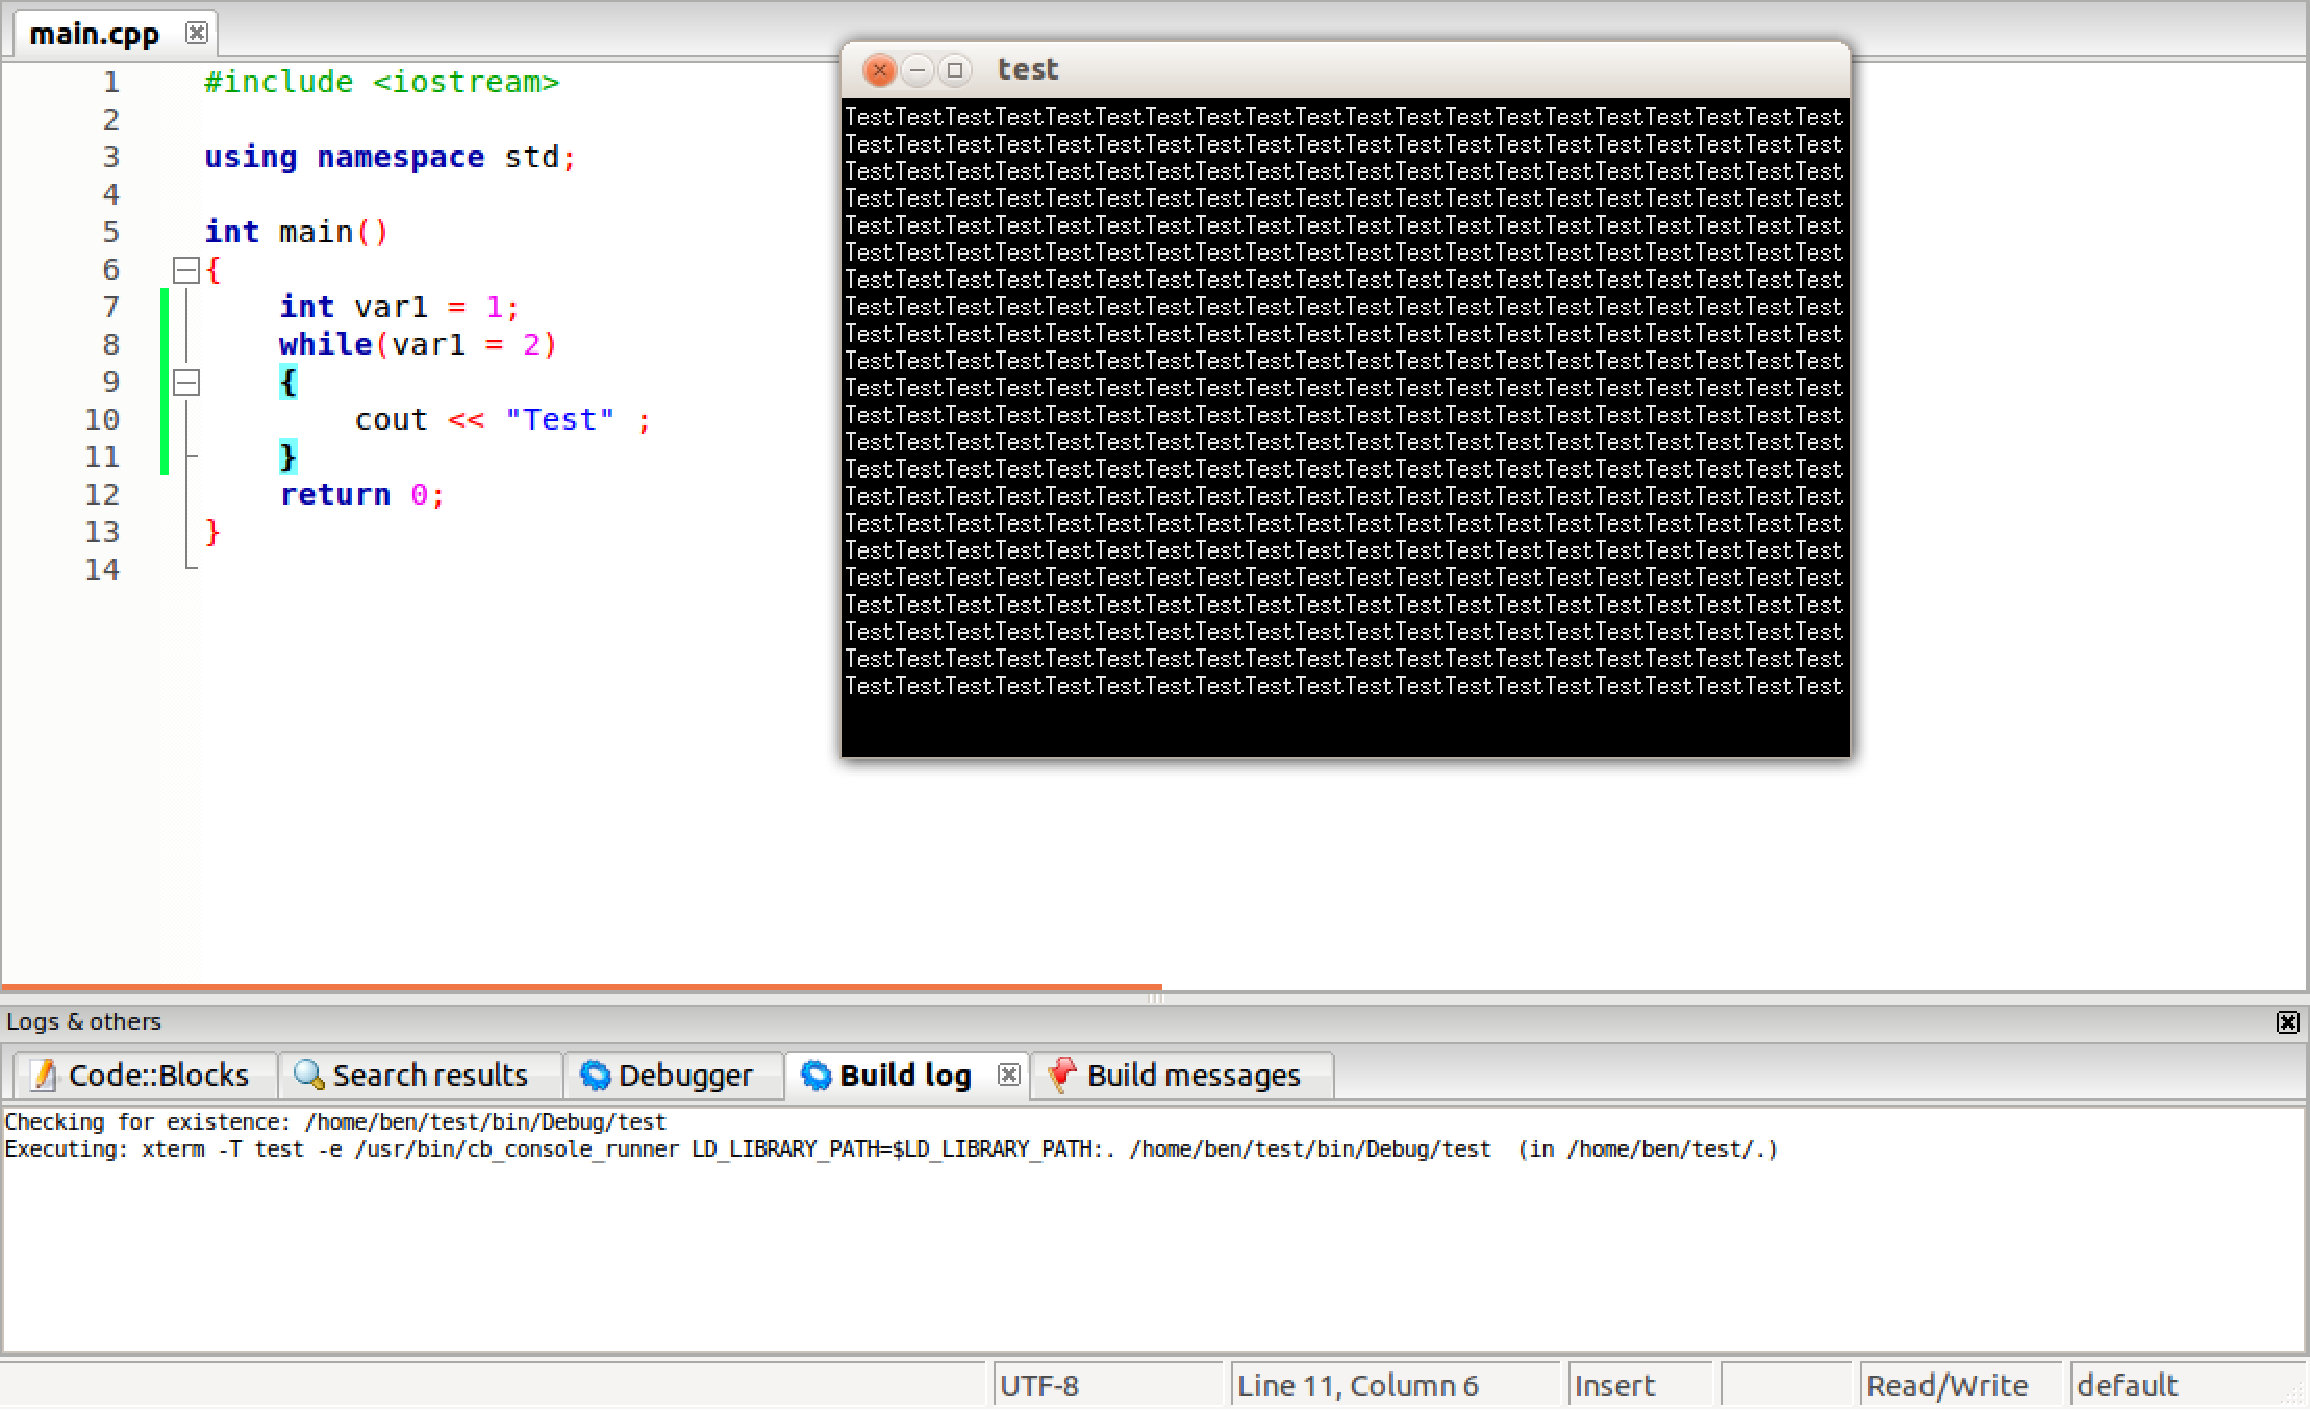
\includegraphics[width=\textwidth]{diagrams/fig-netbeans-infinite-loop.pdf}
  \caption{An infinite loop in the NetBeans development environment} \label{fig-netbeans-infinite-loop} 
\end{figure}


\LevelD{Review Questions}
\begin{enumerate}
	\item Consider the following function:
	
\noindent\begin{minipage}{\linewidth}\begin{lstlisting}
double average (double s1, double s2, double s3, s4);
{
  retun s1+s2+s3+s4/4
}
\end{lstlisting}\end{minipage}

		\begin{enumerate}
		\item Find the syntax errors in the function.
		\item There is a logic error in the function. What is it? How does it affect the output of the code?
		\end{enumerate}

  \item The below program compiles, but does not get the result the programmer wanted. Why?

\noindent\begin{minipage}{\linewidth}\begin{lstlisting}
int main()
{
  int shots, goals, saves;
  double save_perc;
  char cont;

  cout.unsetf(ios::fixed);
  cout.unsetf(ios::showpoint);

  cout << "Enter the number of shots on goal:\t";
  cin >> shots;
  cout << "Enter the number of goals scored:\t";
  cin >> goals;
  cout << endl;

  saves = shots - goals;

  // Hockey shows save % as decimal to three places
  save_perc = (saves / shots); 
  cout << "If there were " << shots << " shots and " 
    << goals << " goals, " 
    << "then the goalie's save percentage was ";

  cout.setf(ios::fixed);
  cout.setf(ios::showpoint);
  cout.precision(3);
  
  cout << save_perc << endl << endl;
  return 0;
}
\end{lstlisting}\end{minipage}


\end{enumerate}

\LevelD{Review Answers}

\LevelD{Further Reading}

\begin{itemize}
\item \url{~}
\item \url{~}
\item \url{~}
\end{itemize}	


%     \LevelC{Testing}
%			\label{chap_testing}
%      \input{chap_testing.tex}

% \LevelA{Section 4}
%   \LevelB{Chapters}
     \LevelC{The Preprocessor}
			\label{chap_preproc}
      Preprocessor directives are lines of code that are executed before the compilation of the code begins. 
These directives are like getting everyone in a room before starting a project or doing warmups before running a race. 
One of the most frequently-used preprocessor directives is \Code{\#include}.

When we want to include in our code a system library or some other file, we use the keyword \Code{\#include} followed by the library name or the file name. 
The way we distinguish between including libraries and including files is with angle brackets and quotes, respectively. 
For example, when we want to use objects like \Code{cout} or \Code{cin}, we need to include the \Code{iostream} library like so: 

\begin{lstlisting}
#include <iostream> 
\end{lstlisting}

If we want to include a file, such as a file named \Code{myFile.h}, we can write: 

\begin{lstlisting}
#include "myFile.h"
\end{lstlisting}

However, when we include files, they must be in the same directory as the file where the \Code{\#include} appears. 
We discuss the Standard Template Library in Chapter \ref{chap_stl}, and include a short sample of other libraries below:

\begin{table}[tb]
	\centering
		\begin{tabular}{| l | p{0.8in} | p{2in} |}
		\hline
			\textbf{Library} & \textbf{Provides} & \textbf{Some common uses} \\ \hline
			
			\Code{<iostream>} & Input/output stream objects & \Code{cout}, \Code{cin}: see Chapters~\ref{chap_input}~and~\ref{chap_output} \\ \hline
			\Code{<cstdlib>} & The C standard library & \Code{rand()}, \Code{abs()}, \Code{NULL} \\ \hline
			\Code{<math>} & Mathematical functions & \Code{pow()}, \Code{sqrt()}, \Code{cos()}, \Code{tan()}, \Code{sin()}: see Chapter~\ref{chap_advancedarith} \\ \hline
			\Code{<iomanip>} & Input/output manipulation & \Code{get\_money()}, \Code{get\_time()}, \Code{put\_time()} \\ \hline
			\Code{<ctime>} & Time-related functions & \Code{clock()}, \Code{time()}, \Code{ctime()} \\ \hline
			\Code{<string>} & The \Code{string} class & See Chapter~\ref{chap_string} \\ \hline
			\Code{<fstream>} & File input and output streams & See Chapter~\ref{chap_file_io} \\ \hline
				
		\end{tabular}
\end{table}

%TODO: #if, #ifdef, #ifndef, #define, etc.


\LevelD{Review Questions}

\LevelD{Homework Questions}

\LevelD{Review Answers}

\LevelD{Homework Answers}

\LevelD{Further Reading}

\begin{itemize}
\item \url{~}
\item \url{~}
\item \url{~}
\end{itemize}	




     \LevelC{Advanced Arithmetic}
			\label{chap_advancedarith}
      Advanced arithmetic in C++ includes mathematics that can't be used in code without the use of the \Code{<cmath>} library. 
This is mathematics that goes above and beyond the primitive operations: addition (\Code{+}), subtraction (\Code{-}), multiplication (\Code{*}), and division (\Code{/}). 
As we have seen before, some simple arithmetic might look like:
	
\noindent\begin{minipage}{\linewidth}\begin{lstlisting}
int x;
x = 1;
x += 5;
\end{lstlisting}\end{minipage}
	The variable \Code{x} is declared as an integer. 
	The next line sets it to one. 
	The \Code{+=} operator adds five to \Code{x}, which makes \Code{x} contain six.
	
Doing simple operations like these does not require any special libraries or unusual commands. 
Any compiler can look at a \Code{+}, \Code{-}, \Code{*}, or \Code{/} in a line of code and know exactly what the programmer 
expects to happen. 
Some math requires a little extra help, though. 
In this case, help is the \Code{<cmath>} library.
 
\Code{<cmath>} is a library that is needed for trigonometric, hyperbolic, exponential, logarithmic, rounding, and absolute value functions. 
The \Code{<cmath>} library is designed to make your life simple and to make complicated mathematics easier in C++. 
Using the \Code{<cmath>} library in code is as simple as including it at the top of your source code file with the rest of your libraries. 
For example:

\noindent\begin{minipage}{\linewidth}\begin{lstlisting}
#include <iostream>	
#include <cmath>
\end{lstlisting}\end{minipage}

After the inclusion of the \Code{<cmath>} library, you can use certain mathematical functions in your code such as \Code{pow(x, y)}, which raises the parameter \Code{x} to the power of parameter \Code{y}, and \Code{sqrt(z)}, which returns the square root of \Code{z}. 
In your first few C++ programs you will probably not use the more advanced mathematical functions included in the \Code{<cmath>} library, but for a full list of the functions provided in \Code{<cmath>}, refer to ``Further Reading'' at the end of this chapter. 

\LevelD{Examples}

\LevelE{\Code{pow()}}
\Code{pow} is the function called when you want to raise a value or variable to a certain power. 
Take a look at the code below and we'll break it down line by line.

\noindent\begin{minipage}{\linewidth}\begin{lstlisting}
int x, y;
x = 4;
y = pow(x + 1, 3) + 6;
\end{lstlisting}\end{minipage}

	First, we are declaring two variables: \Code{x} and \Code{y}. 
	After that we set \Code{x} to 4. 
	Now we get to a more interesting section of code. 
	We are asking the compiler to raise the value of \Code{x} plus 1 to the power of 3, add 6, and then place the result in \Code{y}. 
	
	To use the \Code{pow} function, you must understand its syntax. 
	Here is the breakdown:

\noindent\begin{minipage}{\linewidth}\begin{lstlisting}
pow (starting value, power being raised)
\end{lstlisting}\end{minipage}

 	So, for \Code{pow(x + 1, 3) + 6}, we are raising the starting value \Code{x}~+~1 to the power of 3. 
 	Before the power of 3 is applied, 1 is added to \Code{x}. 
 	In this case it is the simple operation of 4+1, which yields 5. 
 	After we get 5, we raise it to the 3\textsuperscript{rd} power to get a value of 125. 
 	After we reach the value of 125 we are finished with the \Code{pow} function and resume using normal operators when we add 6 to 125 resulting in the final value of 131.  
	
	Undoubtedly there are more complicated uses of the \Code{pow} function, such as multiple uses of \Code{pow} in the same line of code. 
	You might use multiple \Code{pow} operations in code that calculates the length of one side of a triangle using the Pythagorean Theorem. 
	Look at the following code and see if you can figure out what the output value would be:

\noindent\begin{minipage}{\linewidth}\begin{lstlisting}
int x, y, z;
x = 3;
y = x + 1;
z = pow(x, 2) + pow(y, 2);
cout << z;
\end{lstlisting}\end{minipage}

	If you got 25, then you have the right answer! 
	After initializing the variables \Code{x} and \Code{y} and setting their values (3 for \Code{x} and \Code{x}+1 for \Code{y}), we raise each value to the power of 2. 
	For visual reference,

\noindent\begin{minipage}{\linewidth}\begin{lstlisting}
z = pow (3, 2) + pow (x+1, 2);
\end{lstlisting}\end{minipage}
results in

\noindent\begin{minipage}{\linewidth}\begin{lstlisting}
z = 9 + 16;
\end{lstlisting}\end{minipage}	
	
	\Code{z}'s value is set to 25. 
	The \Code{pow} function is simple to use and can make the program simpler from a readability standpoint.

\LevelE{\Code{sqrt()}}
	Square roots are calculated using the \Code{sqrt} function. 
	Take a look at the example below to see how it is called in a program:

\noindent\begin{minipage}{\linewidth}\begin{lstlisting}
int a, b;
a = 25;
b = sqrt(a);
\end{lstlisting}\end{minipage}

	\Code{sqrt} is simpler than \Code{pow} in that it only requires one parameter. 
	Since \Code{sqrt} returns a \Code{double}, you should usually assign the result to a \Code{double} variable, but in this example, \Code{sqrt} returns exactly 5, so it is implicitly converted to an \Code{int} without any issues. 
	
	There are cases where both \Code{sqrt} and \Code{pow} are used in the same formula, such as when calculating the distance between two points. 
	When writing such code, it is very important to keep track of the parentheses and to use correct syntax. 
	One such syntax mistake is made when programmers think that C++ syntax is the same as algebraic syntax. 
	This is \emph{not} the case in C++!

\noindent\begin{minipage}{\linewidth}\begin{lstlisting}
int x = (5)(pow(3, 3)); // Incorrect syntax!
\end{lstlisting}\end{minipage}

When the compiler sees this, it doesn't view it as multiplication, but instead as (according to a professional), ``function shenanigans.'' 
It is important to be explicit with mathematical symbols in C++. 
So instead of the incorrect code above, use:

\noindent\begin{minipage}{\linewidth}\begin{lstlisting}
int x = 5 * (pow (3, 3));
\end{lstlisting}\end{minipage}

As an example, we will use code to compute the distance between the two points $(4,4)$ and $(6, 10)$ on a plane.
Refer to the code and the diagrams if you do not understand or get lost.

\noindent\begin{minipage}{\linewidth}\begin{lstlisting}
int x1, x2, y1, y2;
float dist;
x1 = 4;
y1 = 4;
x2 = 6;
y2 = 10;

dist = sqrt(pow (x2 - x1, 2) + pow (y2 - y1, 2));
cout << dist;
\end{lstlisting}\end{minipage}
	
	Your final answer after the calculation is executed is roughly $6.342555$. 
	Without the help of the advanced arithmetic operations, getting to this result would be a difficult, long, drawn-out process. 
	\Code{pow} and \Code{sqrt} are handy functions that make life easier, all with the help of the \Code{<cmath>} library.

\LevelE{Modulo}
The modulo operator (the percent sign: \Code{\%}) finds the remainder, or what was left over from division. 
This program uses the modulo operator to find all prime numbers (all the numbers that never have a remainder of 0 when divided by every number except 1 and itself) that can be held by an \Code{int}.

\noindent\begin{minipage}{\linewidth}\begin{lstlisting}
#include <iostream>
using namespace std;
int main()
{
  int testprime = 0, divby = 0, remainder = 0;
  bool isprime;
  cout << "Prime Number Finder" << endl;
  while(testprime < 2147483647) //The maximum for int
  {
    isprime = true;
    testprime++;
    for(divby = 2; divby < testprime; divby++)
    {
      // store the remainder of the current number when divided by divby
      remainder = testprime % divby; 
      if (remainder == 0) //If the number is not prime
      {
        isprime = false;
        break;
      }
    }
    if (isprime) //If it passes the test, it is prime.
    {
      // tell us what the prime number is.
      cout << " " << testprime; 
    }
  }
	return 0;
}
\end{lstlisting}\end{minipage}

\LevelD{Review Questions}
\begin{enumerate}
\item Which \Code{\#include} library is needed to use advance arithmetic operators?

\item Write C++ code to calculate $2^9$.

\item Write a statement to set the value of a variable of type \Code{double} to the square root of 10001.
\end{enumerate}

\LevelD{Homework Questions}
Complete the code below to find the length of the hypotenuse of a right triangle (remember that $a^2 + b^2 = c^2$) given the lengths of the other two sides. What is the final output of your code?

\noindent\begin{minipage}{\linewidth}\begin{lstlisting}
#include <iostream>
// Add necessary libraries here

using namespace std;

int main()
{
  double a = 3.0, b = 4.0;
  double c;
	//
	// Finish the program...
	//
  cout << "The hypotenuse of the right triangle is "
       << c << endl;
}
\end{lstlisting}\end{minipage}


\LevelD{Review Answers}
\begin{enumerate}
\item \Code{\#include <cmath>} must be included to include advanced operators.
\item \Code{pow(2, 9)}
\item \Code{double b = sqrt(10001);}
\end{enumerate}

\LevelD{Homework Answers}

\noindent\begin{minipage}{\linewidth}\begin{lstlisting}
#include <iostream>
#include <cmath>

using namespace std;

int main()
{
  float a = 3.0, b = 4.0;
  double c;
	
  a = pow(a, 2);
  b = pow(b, 2);
  c = sqrt(a+b);

  cout << "The hypotenuse of the right triangle is "
       << c << endl;
}
\end{lstlisting}\end{minipage}

The final output of the code is: 

\Code{The hypotenuse of the right triangle is 5.0}


\LevelD{Further Reading}
\begin{itemize}
\item \url{http://pages.cpsc.ucalgary.ca/~jacob/Courses/Fall00/CPSC231/Slides/08-Arithmetic.pdf}
\item \url{http://www.cplusplus.com/reference/cmath/}
\end{itemize}

     \LevelC{File I/O}
			\label{chap_file_io}
      % This work by Jeremy A. Hansen is licensed under a Creative Commons 
% Attribution-NonCommercial-ShareAlike 3.0 Unported License, 
% as described at http://creativecommons.org/licenses/by-nc-sa/3.0/legalcode

\Keyword{File I/O} refers to the input and output (I/O) from and to files. 
So far we have been using \Code{cin} to get input from the keyboard and \Code{cout} to output to the screen. 
Just like output can be sent to the screen, output can be sent to a file. 
Input can be taken either from a keyboard or from a file. 
Input and output is handled in the program through objects called \Keyword{streams}. 
This chapter will discuss how to take input from a file and send output to the same file or a different one. 

File I/O is useful because files provide a way to store data permanently. 
With keyboard input and screen output, the data is temporary and goes away once the program is finished.
When it comes to files, the data is there for us and we do not have to waste our time typing it over and over again. 

\LevelD{I/O Streams}

If data is flowing into your program it is called an \Keyword{input stream}. 
If data is flowing out of the program it is called an \Keyword{output stream}. 
We have actually been using both types of streams already! 
\Code{cin}, which handles a flow of data from the keyboard, is an input stream and \Code{cout}, which produces a flow of data to the screen, is an output stream. 
If an input stream object is connected to a file, then the program can get its input from that file. 
Similarly, an output stream object can send data to the screen or to a file. 
A file can be opened for both reading and writing, in which case it can be accessed by both input and output streams.

\LevelD{File I/O}

When the program opens a file for input, the program is reading from the file. 
When the program opens a file for output, the program is writing to the file. 
C++ provides us with the \Code{ifstream}, \Code{ofstream}, and \Code{fstream} classes for reading from and writing to files. 
All of these classes are available through the \Code{fstream} library, which means we must \Code{\#include} it in our code in order to use them:

\noindent\begin{minipage}{\linewidth}\begin{lstlisting}
#include <fstream>
\end{lstlisting}\end{minipage}

The \Code{ofstream} type (read that as ``\textbf{o}utput \textbf{f}ile \textbf{stream}'') is used to write data to files. 
The \Code{ifstream} type (``\textbf{i}nput \textbf{f}ile \textbf{stream}'') is used to read data from files. 
Objects of type \Code{fstream} (``\textbf{f}ile \textbf{stream}'') can combine the behavior of \Code{ifstream} and \Code{ofstream} and allow us to both read from and write to files.

The \Code{cin} and \Code{cout} objects are already declared for you. 
However, in order to use \Code{ifstream}, \Code{ofstream} and \Code{fstream} objects, you must declare one like you would any other variable. 
Declaring these objects looks like this:

\noindent\begin{minipage}{\linewidth}\begin{lstlisting}
//Declares a variable of type ifstream named input
ifstream inFile; 
//Declares a variable of type ofstream named output
ofstream outFile; 
\end{lstlisting}\end{minipage}

The variable \Code{inFile} will deal with getting input from a file, while the variable \Code{outFile} will deal with outputting data to a file. 

Every file on a computer has its own name and a location (or \Keyword{path}).
An example of a text file name is \Code{TextFile.txt} and its location in a Windows operating system might be \Code{c:\textbackslash storage\textbackslash TextFile.txt}. 
In a UNIX-based operating system, the same file might be in \Code{/home/user1/TextFile.txt}. 
Regardless of the operating system, we need to know the file's path in order to tell the program where to find the file. 

\LevelD{Opening and closing a File}

Before we can even start reading from and writing to a file we must open it. 
In order to open a file you must first make an object of type \Code{ifstream}, \Code{ofstream}, or \Code{fstream} just like we did earlier. 
We open a file using a member function named \Code{open}. 
The \Code{ofstream} object will create a file for you if the file you're opening for output does not exist.
Otherwise, if the file already exists, the \Code{open} function will erase existing data in the file by default. 
The following example demonstrates how to open files for both input and output:

\noindent\begin{minipage}{\linewidth}\begin{lstlisting}
#include <iostream> //For cin and cout 
#include <fstream> // For ifstream and ofstream
		
using namespace std;
		
int main ()
{
  //Declares a variable of type ifstream called inFile
  ifstream inFile; 
  //Declares a variable of type ofstream called outFile
  ofstream outFile; 
	
	//Opens text file for input
  inFile.open("TextFile.txt"); 
  //Creates text file for output
  outFile.open("OutputTextFile.txt"); 
	
  return 0;
}
\end{lstlisting}\end{minipage}

%TODO: Add an example of appending data to an ofstream

Once you are done with the file, it is good practice to close it. 
Closing the file disconnects it from the program and prevents the program from continuing to read from or write to the file. 
If the program ends normally or crashes, the files will be automatically closed. 
Closing files is even simpler than opening them. 
All you need to do is use the \Code{close} function with empty parentheses. 
For example, to close both \Code{inFile} and \Code{outFile}:

\noindent\begin{minipage}{\linewidth}\begin{lstlisting}		
inFile.close();
outFile.close();
\end{lstlisting}\end{minipage}
	
\LevelD{Reading from a File}

We use the \Code{ifstream} class to read data from a file. 
Instead of having a user input data from the keyboard, we now input the data from a file. 
As you recall from earlier in the book, we used \Code{cin} with \Code{>>}, the \Keyword{extraction operator}. 
This is the operator we use when we would like get input from the keyboard and it is also used with \Code{ifstream} objects. 
Once we have declared our variable of type \Code{ifstream} and opened a file, we can use it to input data. 
Using this is very similar to \Code{cin} except we replace \Code{cin} with the name of our variable.
For example: \nopagebreak[4]

\noindent\begin{minipage}{\linewidth}\begin{lstlisting}		
#include <iostream> 
#include <fstream>
	
using namespace std;

int main()
{
  int number=5;
  ifstream inFile;

  inFile.open("TextFile.txt");

  inFile >> number; 
  // The value 5 in number is overwritten
	// by the integer stored in the file

  return 0;
}
\end{lstlisting}\end{minipage}		

This will read in one integer from the file and store it into the variable \Code{number}. 
You can input all different types of data including characters, \Code{double}s, and \Code{float}s. 
Overall, \Code{ifstream} objects are very similar to \Code{cin}---you just have to declare one and remember to use the variable name instead of \Code{cin}.

\LevelD{Writing data to a File}

We use the \Code{ofstream} class to output data to files. 
\Code{cout} outputs data to our screen whereas \Code{ofstream} stores data in files. 
Just like \Code{cout}, \Code{ofstream} objects use \Code{<<}, the \Keyword{insertion operator}. 
Using this is very similar to \Code{cout} except we replace the \Code{cout} with the name of our variable. 
For example: \nopagebreak[4]

\noindent\begin{minipage}{\linewidth}\begin{lstlisting}		
#include <iostream> 
#include <fstream>
		
using namespace std;
int main ()
{
  char Letter = 'A';
  ofstream outFile;

  outFile.open("OutputTextFile.txt");

  outFile << Letter; // Puts the letter 'A' into the file

  return 0;
}
\end{lstlisting}\end{minipage}

This example would write the letter \Code{'A'} to the text file we created named \Code{OutputTextFile.txt}. 
You can also create numeric variables and output them to the file just like:
			
\noindent\begin{minipage}{\linewidth}\begin{lstlisting}
int num = 10;
outFile << num << endl;
\end{lstlisting}\end{minipage}		

This example would output the number 10 and create a new line in the text file we created. 

\LevelD{Introduction to Classes and Objects}
	
We will go into more detail about classes and objects in Chapter \ref{chap_classes} but it is necessary to go over it briefly in this section. 
Both \Code{cin} and \Code{cout} are objects. 
An \Keyword{object} is a variable that has functions built in and may have multiple pieces of data associated with it. 
\Code{ifstream} and \Code{ofstream} are object types that define which operations may be performed on and which data are stored in the objects. 
For example, the function \Code{open()} (along with \Code{close()} and many others) is considered a \Keyword{member function} of \Code{ifstream} and \Code{ofstream}, which means it is a function that is associated with object of those two types. 
Getting a little more into detail, these object types are defined as part of a \Keyword{class}. 
A class is a blueprint for complex data types. 
We already know data types such as integers, \Code{double}s, and \Code{char}s, but using classes, you will be able to design your own data type.

When calling the functions \Code{open} or \Code{close}, you will notice we use a period between the object name and the function. 
We call this the \Keyword{dot operator} and it is used to reference member functions and member variables of a class. 

\LevelD{Other functions}

The \Code{<fstream>} library comes with many functions to help test to see if things are working. 
One example is the \Code{fail()} function. 
We use this function to determine whether the file was opened successfully or not. 
We usually use \Code{if} statements with the function so that if the file does not open correctly we can warn the user. 
For example:

\noindent\begin{minipage}{\linewidth}\begin{lstlisting}
inFile.open("TextFile.txt");
if (inFile.fail())
{ 
  cout << "Failed to open!";
}
\end{lstlisting}\end{minipage}

This will warn the user if the file did not open correctly. 
If the file \emph{did} open correctly, the program would continue without printing the error message.

The next function is the \Code{eof()} (\textbf{e}nd \textbf{o}f \textbf{f}ile) function. 
This function tests to see if the stream has reached the end of the file. 
This function is very useful in order to know when to stop reading from the file. 
For example:

\noindent\begin{minipage}{\linewidth}\begin{lstlisting}
int number;
inFile.open("TextFile.txt");
while (!inFile.eof())
{
  inFile >> number
}
\end{lstlisting}\end{minipage}

This example shows how the \Code{eof()} function can be used in a \Code{while} loop. 
The \Code{while} loop will read integers from the file until the program reaches the end of the file. 
This is useful for gathering all the data from one file. 

The \Code{get()} and \Code{put()} functions are used to read and write single characters, respectively. 
The function \Code{get()} allows the program to read in a single character into a variable of type \Code{char}. 
When we use the \Code{>>} operator, spaces, tabs and newlines---the whitespace characters---around data are skipped automatically. 
However with \Code{get()}, nothing is done automatically, so the whitespace characters can be extracted, too. 
The member function \Code{get()} takes one argument in parentheses that must be a \Code{char} variable. 
For example:

\noindent\begin{minipage}{\linewidth}\begin{lstlisting}
char Character;
ifstream inFile;

cin.get(Character);
//or
inFile.get(Character);
\end{lstlisting}\end{minipage}

This will read in the next character typed on the keyboard or from the file. 
Even if the next character is a space, tab, or newline, the program will store that character in the variable. 

The \Code{put()} function is used to output one character. 
This function takes one argument of type \Code{char} in the parentheses. 
For example:

\noindent\begin{minipage}{\linewidth}\begin{lstlisting}
char Character = '\n'; // newline character
ofstream outFile;

cout.put(Character);
// or
outFile.put(Character);
\end{lstlisting}\end{minipage}

\LevelD{Review Questions}

\begin{enumerate}
\item What do we call the type of object used to control data flowing into your program?
\item What do we call the type of object used to control data flowing out of your program?
\item What header file must you \Code{\#include} in order to use \Code{ifstream} and \Code{ofstream}?
\item What are \Code{ifstream} and \Code{ofstream} used for?
\item How do you declare an \Code{ifstream} object named \Code{input} and an \Code{ofstream} object named \Code{output}?
\item How would you open a file named \Code{TextFile.txt} with an \Code{ifstream} object called \Code{input}?
\item How would you close a file named \Code{TextFile.txt} with an \Code{ofstream} object called \Code{output}?
\item What kind of function is the \Code{eof()} function and what does it do?
\item What are the benefits of using files for input and output?
\item What is the difference between \Code{cin~>>~c;} and \Code{cin.get(c);} if \Code{c} is of type \Code{char}?
\item Write a program that outputs the contents of some file to the screen.
\item Write a program that reads in a text file and prints to the screen the number of times the character \Code{'e'} shows up.
\end{enumerate}

\LevelD{Review Answers}

\begin{enumerate}
\item An input stream
\item An output stream
\item You need to \Code{\#include <fstream>}
\item \Code{ifstream} is used to read data from a file. \Code{ofstream} is used to write data to a file.
\item \Code{ifstream input;}

			\Code{ofstream output;}
\item \Code{input.open("TextFile.txt");}
\item \Code{output.close();}
\item The \Code{eof()} function is a member function. It returns \Code{true} if the program has reached the end of the file.
\item File input and output are useful because files provide a way to store data permanently. With keyboard input and screen output, the data is temporary and disappears once the program is finished. The data stored in files on the other hand remains the same until another program changes it. Also, an input file can be used by many programs at the same time without having to store multiple copies or re-enter the data over and over again.
\item The first \Code{cin} statement the next non-whitespace character into \Code{c}, but the call to \Code{cin.get()} stores the next character in \Code{c} whether it is whitespace or not.
\end{enumerate}

\LevelD{Further Reading}

\begin{itemize}
\item \url{http://www.cprogramming.com/tutorial/lesson10.html}
\item \url{http://www.cplusplus.com/doc/tutorial/files/}
\item \url{http://www.tutorialspoint.com/cplusplus/cpp_files_streams.htm}
\end{itemize}	


     \LevelC{Pointers}
			\label{chap_pointers}
      % This work by Jeremy A. Hansen is licensed under a Creative Commons 
% Attribution-NonCommercial-ShareAlike 3.0 Unported License, 
% as described at http://creativecommons.org/licenses/by-nc-sa/3.0/legalcode

Pointers do just what they sound like they do. 
They point to a space in memory, usually a location occupied by a variable. 
A pointer is an address in memory. 
The pointer itself is a variable, but it also refers to a variable. 
It is declared using an asterisk following the data type:

\noindent\begin{minipage}{\linewidth}\begin{lstlisting}
int *ptr; 
\end{lstlisting}\end{minipage}

The variable named \Code{ptr} is of type \Code{int*}, an ``integer pointer'' that stores the address of a variable of type \Code{int}.

To indicate that a pointer variable is not pointing toward any usable data, we often set its value to \Code{NULL}, which is defined as zero when you \Code{\#include <cstdlib>}:

\noindent\begin{minipage}{\linewidth}\begin{lstlisting}
int *ptr = NULL;
\end{lstlisting}\end{minipage}

C++11 provides a dedicated null pointer object called \Code{nullptr} that can be used similarly:

\noindent\begin{minipage}{\linewidth}\begin{lstlisting}
int *ptr = nullptr;
\end{lstlisting}\end{minipage}

There are two operators used in conjunction with pointers. 
The \Code{*} operator, beyond being used for multiplication and for pointer declarations, also acts as the \Keyword{dereference operator}. 
The dereference operator changes the pointer into the value it is pointing to.
It ``follows'' the address stored in the pointer and returns whatever is in that location.

The \Code{\&} operator is the \Keyword{reference operator}. 
The dereference operator returns the memory address of the variable it precedes. 
You will use this to produce a pointer to the indicated variable. Let's declare pointer \Code{p} and use it:

\noindent\begin{minipage}{\linewidth}\begin{lstlisting}
int *p;       // Declare an int pointer
int var1 = 2; // Declare an int, set it to 2
p = &var1;    // Take the address of var1 and store it in p
cout << *p;   // Go to the address stored in p;
              // return the value; print it out
\end{lstlisting}\end{minipage}

\noindent The output of this code is:

\noindent \Code{2}

Here is a slightly longer example:

\noindent\begin{minipage}{\linewidth}\begin{lstlisting}
int *p;
int var1 = 2;
int var2 = 4;
p = &var1; // Take the address of var1 and store it in p
*p = var2; // Go to the address stored in p; 
           // assign it the value stored in var2

// The preceding two lines are equivalent to var1 = var2
cout << *p << endl;
cout << var1 << endl;
cout << var2 << endl;
\end{lstlisting}\end{minipage}

The output of this code is:

\noindent \Code{4}

\noindent \Code{4}

\noindent \Code{4}

\begin{figure}[tb]
  \centering
  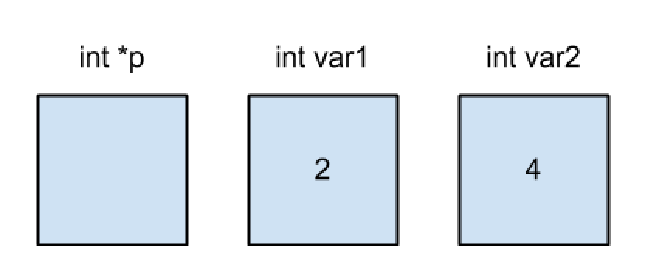
\includegraphics[width=0.6\textwidth]{diagrams/pointer-example-1.pdf}
  \caption{The state of the variables after lines 1-3} \label{fig:pointer-example-1} 
\end{figure}

\begin{figure}[tb]
  \centering
  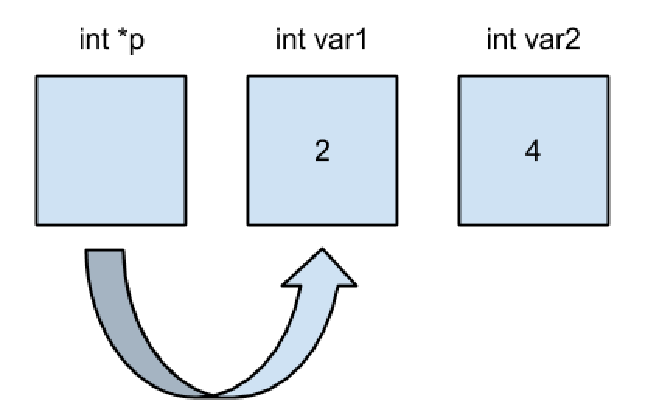
\includegraphics[width=0.6\textwidth]{diagrams/pointer-example-2.pdf}
  \caption{The state of the variables after line 4} \label{fig:pointer-example-2} 
\end{figure}

\begin{figure}[tb]
  \centering
  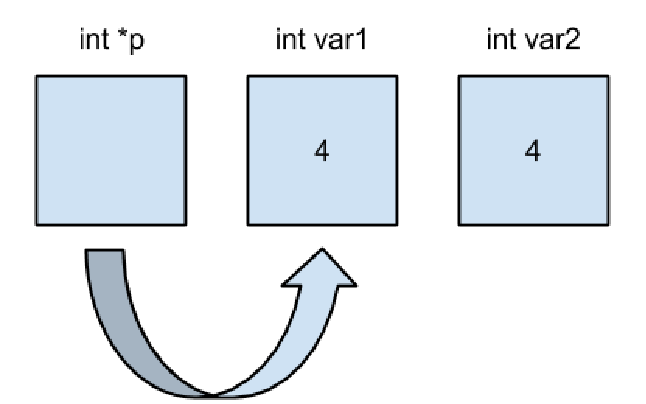
\includegraphics[width=0.6\textwidth]{diagrams/pointer-example-3.pdf}
  \caption{The state of the variables after line 5} \label{fig:pointer-example-3} 
\end{figure}

Figure \ref{fig:pointer-example-1} shows the state of the variables in the second example after they are declared and initialized (lines 1-3).
After the fourth line is executed, \Code{p} will store the address of \Code{var1}. Figure \ref{fig:pointer-example-2} shows the state of the variables.
After the fifth line of code is executed, the location where \Code{p} points is assigned the value stored in \Code{var2}.
Since \Code{p} contains the address of \Code{var1}, \Code{var1} receives that value. Figure \ref{fig:pointer-example-3} shows the state of the variables.

Use caution when declaring pointers.
If you are declaring more than one pointer in a single line, make sure to indicate each pointer variable with the \Code{*} before the variable name.  
Here is a correct declaration of two pointers:

\noindent\begin{minipage}{\linewidth}\begin{lstlisting}
int *p, *q;
\end{lstlisting}\end{minipage}

This results in an integer pointer named \Code{p} and an integer pointer named \Code{q}. 
Contrast that with the below code:

\noindent\begin{minipage}{\linewidth}\begin{lstlisting}
int *p, q;
\end{lstlisting}\end{minipage}

This results in an integer pointer named \Code{p} and an integer named \Code{q}. 
An equivalent way to write the above is: \nopagebreak[4]

\noindent\begin{minipage}{\linewidth}\begin{lstlisting}
int q, *p;
\end{lstlisting}\end{minipage}

\LevelD{Review Questions}

\begin{enumerate}
	\item What is the output of the following code? \nopagebreak[4]

\noindent\begin{minipage}{\linewidth}\begin{lstlisting}
int *a, b, c;
a = &b;
b = 5;
c = 1;
b = b - b;
c = b * b;
*a = c - *a;
a = &c;
*a = c - 7;
c = c + c;
*a = *a + b;
c = c + b;
b = c - 3;
c = *a - 7;
cout << *a << endl;
cout << b << endl;
cout << c << endl;
\end{lstlisting}\end{minipage}
	\item What is the output of the following code? \nopagebreak[4]

\noindent\begin{minipage}{\linewidth}\begin{lstlisting}
int a, b, *c;
a = 7;
b = 4;
c = &a;
a = *c - a;
*c = *c + 4;
a = b + a;
c = &b;
a = a - b;
*c = b + a;
*c = *c - 1;
a = a * 1;
a = b - *c;
a = a - *c;
cout << a << endl;
cout << b << endl;
cout << *c << endl;
\end{lstlisting}\end{minipage}
\end{enumerate}

\LevelD{Review Answers}

\begin{enumerate}
	\item \Code{-21}

				\Code{-17}

				\Code{-21}

	\item \Code{-7}

				\Code{7}

				\Code{7}
\end{enumerate}

%\LevelD{Further Reading}

%\begin{itemize}
%\item ~
%\item ~
%\item ~
%\end{itemize}	

     \LevelC{Dynamic Data}
			\label{chap_dynamic}
      % This work by Jeremy A. Hansen is licensed under a Creative Commons 
% Attribution-NonCommercial-ShareAlike 3.0 Unported License, 
% as described at http://creativecommons.org/licenses/by-nc-sa/3.0/legalcode

Up to this point, we have only discussed variables that are set up at compile time. 
Allocating space for variables at compile time is adequate in many cases, but occasionally a program will need to allocate space for data in memory while it is running. 
Consider the following code:

\noindent\begin{minipage}{\linewidth}\begin{lstlisting}
int arraySize;
cout << "Enter the number of elements you want in the array: ";
cin >> arraySize;
int myArray[arraySize]; // We want to create an array with arraySize elements
// SYNTAX ERROR!
\end{lstlisting}\end{minipage}

In order to allocate the space for \Code{myArray}, the compiler needs to know how many elements make up the array so that there is enough room in memory to accommodate the array. 
Unfortunately, the value of \Code{arraySize} is not known until the user enters something on the keyboard \emph{after the program has started running} and as a result, the compiler returns a syntax error. 

In C++, pointers are used to keep track of dynamically-allocated data:

\noindent\begin{minipage}{\linewidth}\begin{lstlisting}
float *fPtr = NULL; // (1) Declare a pointer to a float, which currently points nowhere
\end{lstlisting}\end{minipage}

In order to dynamically allocate an object of type \Code{float}, we use the \Code{new} operator:

\noindent\begin{minipage}{\linewidth}\begin{lstlisting}
fPtr = new float; // (2)
\end{lstlisting}\end{minipage}

\begin{figure}[tbh]
  \centering
  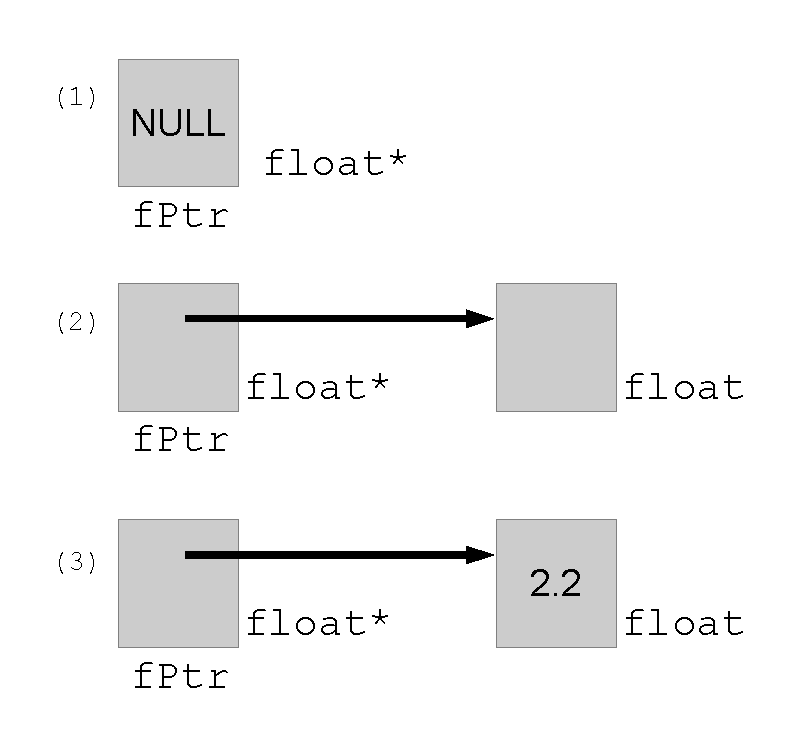
\includegraphics[width=0.7\textwidth]{diagrams/new_operator_diagram_1.pdf}
  \caption{Allocation and dereferencing of pointers} \label{fig:new_operator_diagram_1} 
\end{figure}

The created object of type \Code{float} does not have a name, so the \Code{new} operator returns a \Code{float*} that can be used to access the object. 
This pointer is stored in \Code{fPtr}. 
We use the dereference operator (\Code{*}, that is) to access the data:

\noindent\begin{minipage}{\linewidth}\begin{lstlisting}
*fPtr = 2.2; // (3) Goes to the address at fPtr and stores 2.2 there
cout << "Data at " << fPtr << ": " << *fPtr << endl;
// This outputs: Data at 0x200102b0: 2.2
// Note that the address listed may differ
// Also note the difference between printing fPtr and *fPtr
\end{lstlisting}\end{minipage}

Notice that when a value is assigned to \Code{fPtr}, the pointer is being changed. 
When a value is assigned to \Code{*fPtr} (notice the dereference operator), the floating-point value at the address stored in \Code{fPtr} is changed. 

\begin{figure}[tbh]
  \centering
  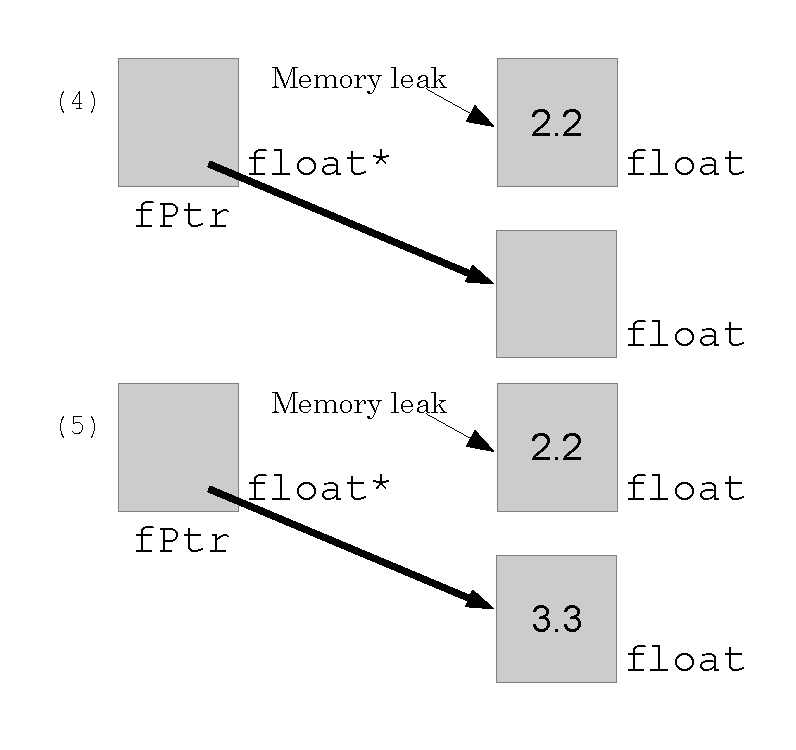
\includegraphics[width=0.7\textwidth]{diagrams/new_operator_diagram_2.pdf}
  \caption{Allocation and memory leaks} \label{fig:new_operator_diagram_2} 
\end{figure}

\noindent\begin{minipage}{\linewidth}\begin{lstlisting}
float *fPtr;
fPtr = new float;
*fPtr = 2.2; // Goes to the address at fPtr and stores 2.2 there
cout << "Data at " << fPtr << ": " << *fPtr << endl;
fPtr = new float; // (4) fPtr now holds the address of a new float object
*fPtr = 3.3; // (5)
cout << "Data now at " << fPtr << ": " << *fPtr << endl;
// This outputs: 
// Data at 0x200102b0: 2.2
// Data now at 0x200483c0: 3.3
\end{lstlisting}\end{minipage}

In this example, the \Code{float} containing the value $2.2$ still resides in memory, but is no longer reachable. 
This condition is called a \Keyword{memory leak}, and results in programs that consume more memory than they require. 
In order to free up the memory properly, we use the \Code{delete} operator:

\noindent\begin{minipage}{\linewidth}\begin{lstlisting}
float *fPtr;
fPtr = new float;
*fPtr = 2.2; // (6) Goes to the address at fPtr and stores 2.2 there
cout << "Data at " << fPtr << ": " << *fPtr << endl;
delete fPtr; // (7) Frees up the dynamically-allocated memory 
// at the address stored in fPtr
\end{lstlisting}\end{minipage}

At this point in the code, \Code{fPtr} can be referred to as a \Keyword{dangling pointer}, since the memory location it refers to is no longer valid, and the pointer just ``dangles'' there, pointing to nothing useful. 

\begin{figure}[tbh]
  \centering
  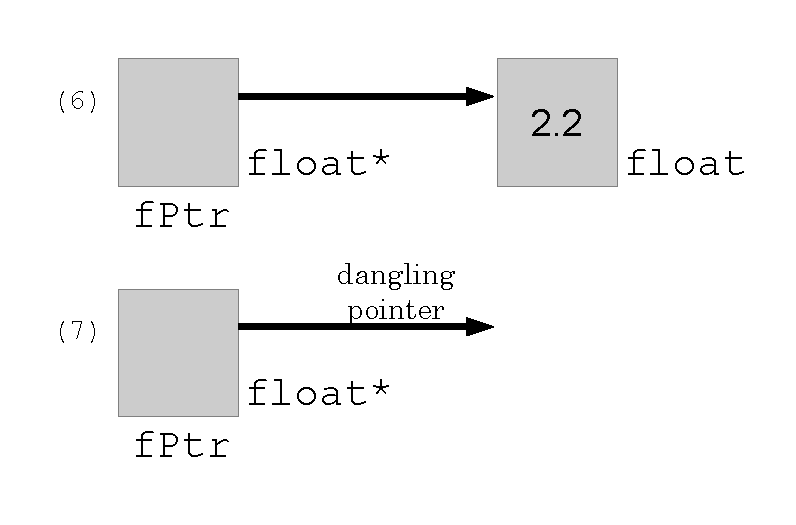
\includegraphics[width=0.7\textwidth]{diagrams/new_operator_diagram_3.pdf}
  \caption{Deallocation and dangling pointers} \label{fig:new_operator_diagram_3} 
\end{figure}
Arrays can be dynamically allocated, too:

\noindent\begin{minipage}{\linewidth}\begin{lstlisting}
float *fPtr = new float[10]; // Allocate an array of ten floats and store their location in fPtr
\end{lstlisting}\end{minipage}

Arrays must be deleted in a similar fashion, but the syntax changes slightly:

\noindent\begin{minipage}{\linewidth}\begin{lstlisting}
delete [] fPtr; // Free up the entire array
\end{lstlisting}\end{minipage}


\LevelD{Review Questions}

\begin{enumerate}
	\item Write code to declare an integer pointer and dynamically allocate an integer. On the next line, assign this dynamically-allocated integer the value 13.

  \item Given the following code, write a few lines that deallocate any dynamically-allocated memory and set all pointer values to \Code{NULL}:

\noindent\begin{minipage}{\linewidth}\begin{lstlisting}
int *a = new int [24];
int *b;
int c;
b = &c;
\end{lstlisting}\end{minipage}


\end{enumerate}

\LevelD{Review Answers}

\begin{enumerate}
\item\noindent\begin{minipage}{\linewidth}\begin{lstlisting}
int *iPtr = new int;
*iPtr = 13;
\end{lstlisting}\end{minipage}

\item\noindent\begin{minipage}{\linewidth}\begin{lstlisting}
delete [] a;
a = NULL;
b = NULL;
\end{lstlisting}\end{minipage}

\end{enumerate}

\LevelD{Further Reading}

\begin{itemize}
\item \url{http://www.cplusplus.com/doc/tutorial/dynamic/}
\end{itemize}	



 \Comment{ % LevelX comment.

 \LevelA{}
   \LevelB{}
     \LevelC{}
     \LevelC{}
     \LevelC{}
     \LevelC{}
     \LevelC{}
     \LevelC{}
     \LevelC{}
     \LevelC{}
 } % End LevelX comment.

% \LevelA{Section 5}
%   \LevelB{Chapters}
%     \LevelC{User-defined types}
%      \input{chap_userdefined.tex}
     \LevelC{Classes and Abstraction}
			\label{chap_classes}
      %Abstract Data Types

%Analogy

Imagine for a second you're behind the wheel of an automobile. 
You're driving along, but do you know your engine is working right if it's not making any horrendous screeching sounds? 
Do you have any idea how your steering actually works when you turn the wheel? 
So long as you can press down on the accelerator to move forward and the steering handles correctly, you probably don't care about the specifics of how things work.

\Keyword{Abstract data types} (ADTs) are the automobiles of C++, and one of the reasons C++ is known as an \Keyword{object-oriented programming language}. 
It's their job to package and obscure the information from the average user, and at the same time make their lives more convenient.
ADTs can be thought of as a group of data of different types that are treated as a single item.
For example, if we wanted to record the name, identification number, age, graduation date, and sex of all of the students on a campus, we could create a new data type named \Code{Student} with those variables.
In the following sections we will show you how to use and define two types of ADTs: structures and classes. 


\LevelD{\Code{struct}s}

A common example of a \Code{struct} is a \Code{Point}. \Code{Point}s store \Code{int}, \Code{float}, or \Code{double} variables \Code{x} and \Code{y}, which represent the position of the \Code{Point} on the the X and Y axes on a coordinate plane. 
Such a \Code{struct} might look like this:

\begin{lstlisting}
		struct Point
		{
			double x;
			double y;
		};
\end{lstlisting}

In the example, the keyword \Code{struct} is used to declare the structure definition while the identifier, the word directly to the right of struct (\Code{Point}), is the structure name and the name of a new data type.
The braces are used just like when we define a function.
However, directly after the closing brace, there must be a semicolon!

Once a structure is defined, it can be used just like the data types \Code{int}, \Code{char}, \Code{string}, and so on. 
For example, we might declare a \Code{Point} structure named \Code{input} like this:

\begin{lstlisting}
		Point input;
\end{lstlisting}

\LevelD{Assigning values to member variables}

Any variable of type \Code{Point} such as the one above is a collection of two variables, \Code{x} and \Code{y}. 
Any variables contained in the \Code{struct} can be accessed by combining the structure name---\Code{input} in our example---followed by a symbol called the \Keyword{dot operator} (the period, \Code{.}) and the member variable's name. 
For example, if we wanted to set \Code{x} in \Code{input}, we would use the dot operator as follows:

\begin{lstlisting}
  input.x = 5;
\end{lstlisting}

\LevelD{Initializing member variables}

% TODO: Add more here

\begin{lstlisting}
Point input(3, 6); 
\end{lstlisting}

\LevelD{\Code{class}es}

\Code{class}es are like \Code{struct}s except \Code{class}es contain both variables and functions, whereas \Code{struct}s only contain variables.\footnote{This has been the conventional way to think about \Code{class}es and \Code{struct}s, but in reality the \emph{only} difference between the two is that members of a \Code{struct} are public by default and members of a \Code{class} are private by default.} 
Also, in a \Code{struct}, member variables are public by default while all members of a \Code{class} are private by default. 
We'll discuss the distinction more in a minute. 
First, let's take a look at an actual \Code{class} definition.

\begin{lstlisting}
class Rectangle
{
  public: 
    Rectangle();	//A default constructor
    void setBase(float length); //These two lines are mutators
    void setHeight(float length);
    float getHeight();	//These two lines are accessors
    float getBase();	
    float findArea();	//These two lines perform operations
    float findPerimeter();
  private:
    float Base;
    float Height;
};
\end{lstlisting}

Notice the similar syntax to the struct. Like struct, first the class keyword is used, followed by the name of the class, and after the closing brace, a (;) semicolon is used. Now, notice the public and private sections of the block. To indicate that a set of member variables or functions is private, we use the private keyword followed by a colon. Everything after the keyword will be considered private. 

\begin{lstlisting}
private:
\end{lstlisting}

If we want to indicate that a set a member variables or functions is public, we use the keyword followed by a colon. Everything after this keyword will be considered public. 

\begin{lstlisting}
public:
\end{lstlisting}

Public and Private Variables and Functions

	The biggest difference between classes and structs is the ability to determine how accessible the data within the class is. A general rule of thumb is to put variables in the private section, where they would be referred to as private member variables, and related functions in the public section, where they would be referred to as public member functions. Private member variables can only be accessed by the member functions, but nowhere else, and public member functions can be used anywhere in the program. 



	Within the above class definition we have seven member functions that we need to define since the variables are private. Each function has a specific purpose to either return or set the variables contained \textit{within the class}, perform an operation using those variables, or initialize the class.

Functions that are declared in the above code that have names starting with the word \Code{get} will be used to access the variables; these functions are called accessors. Functions that are declared in the above code that have names starting with the word \Code{set} will be used to change the variables' values; these functions are called mutators. Accessors and mutators can be named whatever you like, but it is common convention to name them \Code{get} and \Code{set} plus the name of the variable you are accessing or mutating. 

The functions whose names start with \Code{find} all perform operations using the variables. The function named \Code{Rectangle()} is known as a constructor. When a \Code{Rectangle} object is created, it will be initialized according to the rules set in this constructor. By the end of this section, you'll understand how useful these are in object-oriented programming.
	

Defining Member Functions

	First we will describe how to use member functions and private member variables. When we define a member function, all the member variables within the class are also available in the function definition. For example if we define the member function \Code{void setBase(float length);} we would define it like this:

\begin{lstlisting}
void Rectangle::setBase(float length)
{
  Base = length;
}
\end{lstlisting}

	In this code we are able to directly access the member variable \Code{Base} because both the function \Code{setBase()} and the member variable \Code{Base} are a part of the class. Since we are not returning anything to the user, the function is defined as a \Code{void} function. In order to define a member function we have to use a special operator called the \Keyword{scope resolution operator} (\Code{::}). The function is defined by using the return type, the class name, scope resolution operator, then the member function name with any parameters listed just like any other non-class function: 

\begin{lstlisting}
void Rectangle::setBase(float length)
\end{lstlisting}
	

Using Member Functions with Variables

	All member functions have direct access to member variables even if the variable is private. The reason we use mutators is because we do not want the user to have direct access to any variables within the class---we give them indirect access instead. We do this by requiring them to somehow enter a value and then pass that value to the mutator member function in order to set the member variable. That might look like this: 

\begin{lstlisting}
	main()
	{
		Rectangle input;
		float length;
		
		cout << �Please input the length of the base: �;
		cin >> length;
		
		input.setBase(length);
	}
\end{lstlisting}

	In the above code, we create a Rectangle variable and use the dot operator to call a member function, just like we would to access a variable in a struct. After the user is prompted for the length of the base, which is stored in the variable length, we call the function with the dot operator and pass length as a parameter to the function. Using the following function definition:

\begin{lstlisting}
	void Rectangle::setBase(float length)
	{
		Base = length;
	}
\end{lstlisting}

\noindent we are able to pass the value of the variable entered by the user to the \Code{setBase} function which then sets the member variable Base to the entered value. This is how we ``mutate'' member variables in a class using a public member function. 

	In order to retrieve the value of a member variable, we need to create accessor functions. These are defined like this: 

\begin{lstlisting}
	float Rectangle::getBase()
	{
		return Base;
	}
\end{lstlisting}

	When it comes to using accessors, it is very simple. Just match the data type that you want to access, in this case it was a float, and define the member function with that return type. Then, in order to access the variable, all we need to do is use the keyword \Code{return} followed by the identifier. This enables us to access the private variable when we need to. 


Classes and Structs Together

	We can also combine \Code{struct}s and \Code{class}es if need be. For example, if we wanted to take in three points we could create a Triangle class with these points which are individually of type \Code{Point}, a \Code{struct} that contains \Code{x} and \Code{y} variables:

\begin{lstlisting}
	struct Point
	{
		double x;
		double y;
	};
	
	class Triangle
	{
	public:
		//accessors for points a, b, and c
		//mutators for points a, b, and c
	private:
		Point a;
		Point b;
		Point c;
	};
\end{lstlisting}

Here we have the ability to combine a \Code{struct} with a \Code{class} in order to have all three points, \Code{a}, \Code{b}, and \Code{c} that each contain their own variables \Code{x} and \Code{y}. Despite the fact that the variables in the \Code{struct} are public, we cannot access those specific values outside the \Code{Triangle} unless we use a member function. This is because they're still private members of the class \Code{Triangle}, so their scope is limited to functions within the class. If we had a mutator function for \Code{Point a}, it might look like this:

\begin{lstlisting}
	void Triangle::setA(double userX, double userY)
	{
		a.x = userX;
		a.y = userY;
	}
\end{lstlisting}

The values of \Code{userX} and \Code{userY} would have been set elsewhere. In order to access the \Code{x} and \Code{y} coordinates, we must use the dot operator with any of the \Code{Point} objects \Code{a}, \Code{b}, or \Code{c}.


Constructors and Destructors

	Another way to set the values of the variables in a class is through constructors. A constructor is a member function with the same name as the class and cannot be called directly. Constructors are what we use to initialize the variables of the class when it's first created. For example, if we wanted to set default values for a class named \Code{student} defined as: 

\begin{lstlisting}
class student
	{
	public:
		student();
		//accessors
		//mutators
	private:
		string name;
		int age;
		int grad_year;
		string id;
	};
\end{lstlisting}

\noindent we would have a default constructor with the name \Code{student()} without any return type. To initialize the variables in the class through the constructor, we use syntax similar to a function definition:

\begin{lstlisting}
	student::student()
	{
		name = "N/A";
		age = 0;
		grad_year = 0;
		id = "A00000000";
	}
\end{lstlisting}

Overloading Member Functions

	Note that, like other functionS, you can overload any of the functions in a class. Going back to the \Code{Rectangle} example used earlier, take a look at the code below:

\begin{lstlisting}
class Rectangle
		{
		public: 
			Rectangle();	//A default constructor
			Rectangle(float userBase, float userHeight);	//Overloaded constructor
			void setBase(float length); //These two lines are mutators
			void setHeight(float length);
			float getHeight();	//These two lines are accessors
			float getBase();	
			float findArea();	//These two lines perform operations
			float findPerimeter();
		private:
			float Base;
			float Height;
		};
\end{lstlisting}

	Notice the second constructor, \Code{Rectangle(float userBase, float userHeight)}. We define it very similarly to the default constructor:

\begin{lstlisting}
Rectangle::Rectangle(float userBase, float userHeight)
{
	Base = userBase;
	Height = userHeight;
}
\end{lstlisting}



\LevelD{Review Questions}

1. Given the following struct and structure variable:

\begin{lstlisting}
	struct personInfo
	{
		string name;
		int birth_year;
		int birth_month;
		int birth_day;
		int age;
	};

	personInfo info;
\end{lstlisting}

Which of the following are not correct ways to use the dot operator?

	a. info.name
	b. info.age
	c. personInfo.birth_year
	d. information.name
	e. personInfo.birth_year;

2. Consider the following code of the struct:

\begin{lstlisting}
	struct personInfo
	{
		string name;
		int birth_year;
		string birth_month;
		int birth_day;
		int age;
	};
\end{lstlisting}


Which of the following is the correct way to initialize the variables from the \Code{struct} above?

	a. personInfo info = {"Michael", 1996, 3, 24, "sixteen"};
	b. personInfo info = {"Michael", 1996, March, 24, 16};
	c. personInfo info = {"Michael", 1996, "March", 24, 16};
	d. struct info = {"Michael", 1996, "March", 24, 16};



\LevelD{Homework Questions}


1.  Write a program that can store information about animals in a zoo.

You should have a class called Animal and the following private variables.

\begin{lstlisting}
string name; // the name of the animal
int pounds; // the number of pounds of food the animal eats
char animalType; // the type of animal: 'h' for herbivore, 'c' for carnivore
\end{lstlisting}

You should have public member functions that get and set each variable, and a function called \texttt{print()} that prints all the information about the animal.

2. This program will require a struct and a class.

Write a program that can calculate the slope of a line.

You will have a struct called Point with the following variables

\begin{lstlisting}
double x, y;
\end{lstlisting}

You will then have a class called Line, and it will have the following private variables

\begin{lstlisting}
Point a, b;
\end{lstlisting}

Your class should have accessor and mutator functions (set and get), a function that calculates and returns the slope of a line between the two \texttt{Point}s as a \texttt{double}, and a function that outputs the data to the user called \texttt{print()}.



\LevelD{Review Answers}

\LevelD{Homework Answers}

\LevelD{Further Reading}

\begin{itemize}
\item \url{http://pages.cpsc.ucalgary.ca/~jacob/Courses/Fall00/CPSC231/Slides/08-Arithmetic.pdf}
\item \url{http://www.tutorialspoint.com/cplusplus/cpp_classes_objects.htm}
\item \url{http://www.cprogramming.com/tutorial/lesson7.html}
\end{itemize}	

%     \LevelC{Exceptions}
%      \input{chap_exceptions.tex}
     \LevelC{Separate compilation}
			\label{chap_separate}
      Separate compilation is the process of breaking a C++ program into separate files to improve organization. 
Parts of the program can be spread out over a number of different files that are later compiled individually, then \Keyword{linked} using a linker to produce the final, working program. 
When changes are made, only those files with changes need to be recompiled, the result of which can then be relinked with the previously-compiled files. 
This process is nearly invisible in most development environments, which recompile and relink these files automatically.
When the development environment takes care of these details, the user is left with the sole task of making changes where they are needed. 

One of the most basic applications of separate compilation is used when writing abstract data types. 
Recall from Chapter \ref{chap_classes} that there are declaration and definition sections in a \Code{class}. 
The declaration contains class functions and variables, both public and private, while the definition section is where the function definitions and most actual code can be found. 
The process of separate compilation requires the two sections to be split into separate files, each of which is written and maintained separately and later used together to create a working program. 

Declarations will be put into the \Keyword{interface} file or the \Keyword{header file} which typically has a \Code{.h} suffix.
In most code written by novice programmers, there will be only one \Code{class} declaration in each header file. 
To use the \Code{class} in your code elsewhere, you should use \Code{\#include} followed by the file name in double quotes. 
Here is an example of the contents of an interface file called \Code{student.h}:

\begin{lstlisting}
#include <string>

using namespace std;

class student
{
public:
	student();
	int getAge();
	void setAge(int update);
	int getID();
	void setID(int update);
	string getName();
	void setName(string update);
private:
	int age;
	int ID;
	string name;
};
\end{lstlisting}

To use the \Code{student} class in some other source code file, that file should include the following line:

\begin{lstlisting}
#include "student.h" 
\end{lstlisting}

The quotes around \Code{student.h} tell the compiler to find the header file in the same directory as the current file.

The \Keyword{implementation} file will include all the function definitions for the \Code{student} class. 
The implementation file can be called anything the programmer wants, but typically ends with a \Code{.cpp} suffix. 
For example, the implementation file for \Code{student} will probably be \Code{student.cpp}.

To ensure that a new implementation file is compiled into your program, you do not need to \Code{\#include} anything. 
However, the development environment will automatically compile and link the implementation file if it has been added to your project.
The only files that you should \Code{\#include} are header files. 

To avoid linker errors, your files should have safeguards to ensure that classes and functions are not declared more than once within the same program. 
These safeguards are simple, and should be included in each header file. 
For example, we place the following two lines at the top of the file \Code{student.h}:

\begin{lstlisting}
#ifndef STUDENT_H // STUDENT_H could be anything 
#define STUDENT_H // as long as it is unique to this file
\end{lstlisting}

The following line should go at the end of the same file:

\begin{lstlisting}
#endif //STUDENT_H � a reminder about the #ifndef above 
\end{lstlisting}

These three lines do the following:

\begin{enumerate}
\item Test if \Code{STUDENT\_H} has been previously \Code{\#define}d, usually because this header file has been \Code{\#include}d elsewhere.
\item If it has not been \Code{\#define}d, \Code{\#define} it now and proceed with compiling the code between the \Code{\#ifndef} and \Code{\#endif}.
\item Close the \Code{\#ifndef} block. If \Code{STUDENT\_H} was previously defined, skip to the line after this one.
\end{enumerate}

Here is an example of what these lines look like alongside some actual code:

\begin{lstlisting}
#ifndef STUDENT_H
#define STUDENT_H

class student
{
//class declaration because this is an interface file
};

#endif//STUDENT_H
\end{lstlisting}

Following this example will ensure that the \Code{student} class is only defined once.






\LevelD{Review Questions}

\LevelD{Homework Questions}

\LevelD{Review Answers}

\LevelD{Homework Answers}

\LevelD{Further Reading}

\begin{itemize}
\item \url{~}
\item \url{~}
\item \url{~}
\end{itemize}	

     \LevelC{STL}
			\label{chap_stl}
      The Standard Template Library (STL) provides a set of tools beyond those that are provided by the ``base'' C++ language. 
While a comprehensive discussion of the features of the STL is far beyond the scope of this text, there are several libraries that offer extremely important features with which you should become comfortable. 

Note: rather than assuming that 

\begin{lstlisting}
using namespace std;
\end{lstlisting}

\noindent is at the top of every code example, each data type, function, or variable derived from the STL will be shown with the prefix \Code{std::}. 
This highlights which parts of the examples below come from the STL, and which are part of the language.

\LevelD{\Code{\#include <utility>} \\ \Code{\#include <tuple>} (C++11)}

The \Code{pair} class, found in \Code{<utility>}, links two values which may be of different types. 
The \Code{tuple} class, introduced in C++11, links any number of values which may be of different types. 
For example, to link a student's identification number (an integer) and their grade point average (a \Code{float}), we can write:

\begin{lstlisting}
std::pair<int,float> grades = { 112233, 3.81 };
\end{lstlisting}

We can assign different values to the \Code{pair} later with the \Code{make\_pair} function:

\begin{lstlisting}
grades = std::make_pair(123450, 2.79);
\end{lstlisting}

The \Code{first} and \Code{second} members are used to extract the individual components of the \Code{pair}:

\begin{lstlisting}
std::cout << "ID: " << grades.first << " (GPA " 
  << grades.second << ")" << std::endl;
// This prints:
// ID: 123450 (GPA 2.79)
\end{lstlisting}

If we wanted a more complicated set of values linked together, such as a student's name, identification number, grade point average, and major, we could construct the following:

\begin{lstlisting}
tuple<std::string, int, float, std::string> ethan = { "Ethan Allen", 802802, 3.15, "Engineering"};
\end{lstlisting}

Unfortunately, the \Code{tuple} class does not have \Code{first} or \Code{second} members. 
The first and second elements can be retrieved in a slightly more complicated way than with \Code{pair} objects:

\begin{lstlisting}
std::cout << std::get<0>(ethan) << "'s major is " 
  << std::get<3>(ethan) << std::endl;
// This prints:
// Ethan Allen's major is Engineering
\begin{lstlisting}

In the code below, the \Code{get} function returns a reference to the third element (the GPA) of the \Code{tuple ethan}, and sets that value to 3.99:

\begin{lstlisting}
std::get<2>(ethan) = 3.99;
\end{lstlisting}

These types may not be all that useful by themselves, but are often used in conjunction with container classes like \Code{vector} and \Code{map}, described below.

\LevelD{\#include <iterator>}

Iterators are objects that refer to elements within a container object (like \Code{std::vector}, \Code{std::map}, and \Code{std::array}) and allow for traversal through those elements. 
The list of features in iterators vary depending on the container class. 
While the specifics of the iterators vary, most iterators belong to one of the following categories, based on the operations that may be performed on them:

\LevelE{Forward iterators}

\begin{itemize}
	\item Can be incremented to move forward in the container to the next item
	\item Can be dereferenced like a pointer variable
\end{itemize}

\begin{lstlisting}
std::array<int> myArray = { 5, 10, 15, 20, 25 };
std::array::iterator myIterator, arrayEnd;
arrayEnd = myArray.end();

// Demonstrating forward iteration
for (myIterator = myArray.begin(); myIterator != arrayEnd; ++myIterator)
  std::cout << *myIterator << " ";

std::cout << std::endl << "The end!" << std::endl;

// This prints:
// 5 10 15 20 25
// The end!
\end{lstlisting}

\LevelE{Bidirectional iterators}

\begin{itemize}
	\item Everything a forward iterator can do and:
	\item Can be decremented to move backward in the container to the previous item
\end{itemize}

\begin{lstlisting}
std::array<int> myArray = { 5, 10, 15, 20, 25 };
std::array::iterator myIterator, arrayBegin;
arrayBegin = myArray.begin();

// Demonstrating backward iteration
for (myIterator = myArray.end(); myIterator != arrayBegin; --myIterator)
  std::cout << *myIterator << " ";

std::cout << std::endl << "The beginning!" << std::endl;

// This prints:
// 25 20 15 10 5
// The beginning!
\end{lstlisting}

\LevelE{Random access iterators}

\begin{itemize}
	\item Everything a bidirectional iterator can do and:
	\item Can use arithmetic operators to move forward and backward a certain number of items at once
	\item Allows comparisons between iterators to determine relative positions in the container
	\item Can use array-style access to elements in the container
\end{itemize}

\begin{lstlisting}
std::array<int> myArray = { 5, 10, 15, 20, 25 };
std::array::iterator myIterator, arrayEnd;
arrayEnd = myArray.end();
myIterator = myArray.begin();

// Demonstrating random access
std::cout << myIterator[1] << " " << myIterator[3] << std::endl;

// Demonstrating iterator comparisons
if (myIterator < arrayEnd)
  std::cout << "The iterator is not at the end of the array yet";

// Demonstrating arithmetic operations on an iterator
for (myIterator = myArray.begin(); myIterator != arrayEnd; myIterator += 2)
  std::cout << *myIterator << " ";

std::cout << std::endl << "The end!" << std::endl;

// This prints:
// 10 20
// 5 15 25
// The end!
\end{lstlisting}

\LevelD{\#include <vector>}

Vectors are containers similar to arrays that are flexible in size and quite fast. 
While we can use iterators as above, we can also treat the \Code{vector} much like an array.

\begin{lstlisting}
// Start with 10 elements, all with the value 98.6
std::vector<float> temperatures(10, 98.6); 

// The last element has a fever of 103.1 degrees!
temperatures[9] = 103.1; 

for (int i = 0; i < temperatures.size(); i++)
{
  std::cout << "Patient " << i << "'s temperature is " 
    << temperatures[i] << std::endl;
}
\end{lstlisting}

The \Code{vector} class also provides member functions \Code{front()} and \Code{back()} which return references to the first element and the last element in the vector, respectively.
For example:

\begin{lstlisting}
std::cout << "The last patient's temperature is " 
  << temperatures.back() << std::endl;
std::cout << "The first patient's temperature is " 
  << temperatures.front() << std::endl;
\end{lstlisting}

Don't confuse the \Code{back()} and \Code{front()} functions with the \Code{end()} and \Code{begin()} functions. 
The \Code{back()} and \Code{front()} functions return references to the elements, while \Code{end()} and \Code{begin()} return \emph{iterators} pointing to those elements.

\LevelD{\#include <map>}

This library provides one of the STL's associative container object classes. 
An associative container differs from an array in that items in an array are referenced with a number which indicates the item's position in memory:

\begin{lstlisting}
int myArray[10]; // An array of ten integers
myArray[0] = -5; // Set the first integer in the array to -5
\end{lstlisting}

An associative container, on the other hand, can use any data type to reference the items in the container. 
For example, you might choose to use a \Code{string} to reference a collection of \Code{int} items to store a list of students' ages according to their names.

\begin{lstlisting}
std::map<std::string,int> students;
\end{lstlisting}

Perhaps you want to create the object with some initial values:

\begin{lstlisting}
std::map<std::string,int> students = 
  { {"John", 19}, 
    {"Max", 19}, 
    {"Christine", 20}, 
    {"Maria", 18} };
\end{lstlisting}

This code produces a structure like in Figure \ref{fig_studentsmap}. 
With these names and ages paired, we can now retrieve the ages using the names.

%TODO: diagram \label{fig_studentsmap}

\begin{lstlisting}
string name = "Christine";
std::cout << name << " is " << students[name] 
  << " years old." << std::endl;

//This code prints:
//Christine is 20 years old.
\end{lstlisting}

New students may also be added in the following way:

\begin{lstlisting}
students["June"] = 18;
students["Omar"] = 19;
\end{lstlisting}

Objects of type \Code{map} may be iterated, and in C++11, their contents can be printed in a range-based \Code{for} loop as we briefly demonstrate here. 
Each item in the \Code{std::map<std::string, int>} is of type \Code{std::pair<std::string,int>}.

\begin{lstlisting}
for (auto& item : students)
{
  std::cout << item.first << " is " << item.second << " years old." << std::endl;
}

// This code prints:
// John is 19 years old
// Max is 19 years old
// Christine is 20 years old
// Maria is 18 years old
// June is 18 years old
// Omar is 19 years old
\end{lstlisting}



\LevelD{Review Questions}

\LevelD{Homework Questions}

\LevelD{Review Answers}

\LevelD{Homework Answers}

\LevelD{Further Reading}

\begin{itemize}
\item \url{http://en.wikipedia.org/wiki/Standard_Template_Library}
\item \url{http://www.cplusplus.com/reference/stl/}
\item \url{~}
\end{itemize}	


 %\missingfigure{Pictures and figures and tables are a nice touch.}

 %\listoftodos

 %\lstlistoflistings

 \printindex

 \end{document}
